\documentclass[11pt]{now}
           
\usepackage{graphicx}
\usepackage{gensymb}
\usepackage{lscape}
\usepackage{epsfig}
\usepackage{subfigure}
\usepackage{hyphenat}
\usepackage{color}


\begin{document}

\isbn{xxxxxxxxxxxxxx}

\DOI{xxxxxxx}

\abstract{Computational support for sketching is an exciting research
  area at the intersection of design research, human-computer
  interaction, and artificial intelligence. Despite the prevalence of
  software tools, most designers begin their work with physical
  sketches. Modern computational tools largely treat design as a
  linear process beginning with a specific problem and ending with a
  specific solution. Sketch based design tools offer another approach
  that may fit design practice better. This article surveys literature
  related to such tools. First, we describe the practical basis of
  sketching---why people sketch, what significance it has in design
  and problem solving, and the cognitive activities it
  supports. Second, we survey computational support for sketching,
  including methods for performing sketch recognition and managing
  ambiguity, techniques for modeling recognizable elements, and
  human-computer interaction techniques for working with
  sketches. Last we propose challenges and opportunities for future
  advances in this field.}

\articletitle{Computational Support for Sketching in Design: A Review}
            

\authorname1{Gabe Johnson}
\affiliation1{Carnegie Mellon University}
\author1address2ndline{Carnegie Mellon University, }
\author1country{USA}
\author1email{johnsogg@cmu.edu}

\authorname2{Mark D. Gross}
\affiliation2{Carnegie Mellon University}
\author2address2ndline{Carnegie Mellon University, }
\author2country{USA}
\author2email{mdgross@cmu.edu}

\authorname3{Jason Hong}
\affiliation3{Carnegie Mellon University}
\author3address2ndline{Carnegie Mellon University, }
\author3country{USA}
\author3email{jasonh@cs.cmu.edu}

\authorname4{Ellen Yi-Luen Do}
\affiliation4{Georgia Institute of Technology}
\author4address2ndline{Georgia Institute of Technology, }
\author4country{USA}
\author4email{ellendo@gatech.edu}

\journal{sample}
\volume{xx}
\issue{xx}
\copyrightowner{xxxxxxxxx}
\pubyear{2008}
            
\maketitle


\cleardoublepage \pagenumbering{roman}

\tableofcontents

\clearpage

\setcounter{page}{0}
\pagenumbering{arabic}

\newtheorem{theorem}{Theorem}[chapter]
\newtheorem{definition}{Definition}[chapter]


\chapter{Introduction}
\label{sec:introduction}

People often sketch when solving problems.  Some sketches are
personal; others are collaborative. Some sketches help people make
quick calculations and are quickly forgotten; others serve longer-term
purposes. For professional designers, sketching serves as a means for
thinking about problems as much as it does for communicating proposed
solutions. For people who are not designers, sketching is a natural
means for quickly recording spatial information such as directions to
a point of interest.

Design can be seen as an iterative process of problem-framing and
exploring possible solutions within the current conception of the
problem. Sketching allows people to visually represent ideas quickly,
without prematurely committing to decisions. A sketch is not a
contract: it is a proposal that can be modified, erased, built
upon. The rough look of hand-made sketches suggests their provisional
nature.

Some theories of cognition give the human mind two distinct tasks: to
perceive the world via our senses, and to reason about what our senses
provide. In contrast, the late psychologist Rudolf Arnheim argues that
perception and thinking are inseparable: ``Unless the stuff of the
senses remains present the mind has nothing to think
with''~\cite{arnheim-visthink}. Visual thinking is valuable in
evaluating what is and designing what might be. Sketching allows
people to give form to notions that are otherwise imaginary; the act
of seeing fuels the process of reasoning.

The term ``sketch'' is used in many ways in vernacular and academic
work. Some speak of sketching as a process---we sketch out an idea by
talking about it, drawing pictures, or play-acting while considering
possible solutions or problem formulations. Alternately we may use the
term ``sketch'' to mean the product of an exploration, as when we make
a prototype out of modeling clay, cardboard, or code.

In this survey we define a \textit{sketch} based on the utility
hand-made drawings afford: sketches are quickly made depictions that
facilitate visual thinking. In this way, sketches may include
everything from doodles to roughly drawn circuit diagrams to an
architect's quick isometric projection. We restrict neither the
drawing medium nor the subject matter. Sketches are most often
two-dimensional graphic depictions, but often incorporate textual
annotations.

Sketching has been a topic of interest to computer scientists and HCI
practitioners for quite some time. Early efforts such as
Sketchpad~\cite{sutherland-sketchpad} and GRAIL~\cite{ellis-grail}
hinted at the potential of pen based interfaces. In fact, many of
today's sketch-related research challenges were suggested by these
systems 45 years ago.

Recently there has been a recurrence of interest in supporting
sketching with computation. Computers can recognize user input and let
people interact with drawings in ways that are impossible with paper
alone, augmenting the sketching process in various ways. A rough
sketch may contain enough information to infer the user's
intentions. The drawing could then come alive, for example providing a
simulation. Alternately the user's sketch may serve as a search
query. Beyond recognition, a computer can render, rectify, or beautify
a user's sketchy input into some other representation. Computation
also supports editing operations that are impossible with physical
sketches, for example enabling collaborators in different locations to
share an electronic drawing surface.

Researchers from many disciplines have contributed to knowledge about
sketching and computational techniques for supporting it. Their
diversity makes it difficult to get a complete sense of what has been
done on this topic. This review draws from journals, conference
proceedings, symposia and workshops in human-computer interaction,
cognitive science, design research, computer science, artificial
intelligence, and engineering design. These fields certainly overlap;
however research in sketching lacks a unifying publication venue.

Some who study sketching as an element of design practice publish in
the \textit{Design Studies} journal. Sketching has become a recurring
theme at HCI conferences like CHI, UIST, IUI and AVI, and visual
languages conferences such as IEEE's VL and VL/HCC. The Association
for the Advancement of Artificial Intelligence (AAAI) held symposia on
diagrammatic representation and reasoning~\cite{glasgow-diagrams} and
sketch understanding. The community brought together by the AAAI
sketch understanding symposia continues meeting at the annual
Eurographics Sketch Based Interaction and Modeling workshop
(SBIM). Related work has been published in computer graphics venues
such as \textit{Computers \& Graphics} and the Non-Photorealistic
Animation and Rendering conference.  There is also a substantial
amount of work published in various journals for electrical,
mechanical, or software engineering.

Surprisingly, few surveys on sketch recognition and interaction have
been published. Readers interested in pen computing in general may
find Meyers' earlier review helpful~\cite{meyer-pen-review}. That
survey covers pen-related hardware, handwriting recognition, and
presents a brief history of the traditional and computational use of
pens but only briefly mentions sketching. Ward has compiled an online
annotated bibliography of pen computing references that spans most of
the 20$^{th}$ century~\cite{ward-pen-bibliography}.

\section{A brief history of pen and sketching systems}
\label{sec:intro-brief-history}

\begin{figure}[]
   \centering
   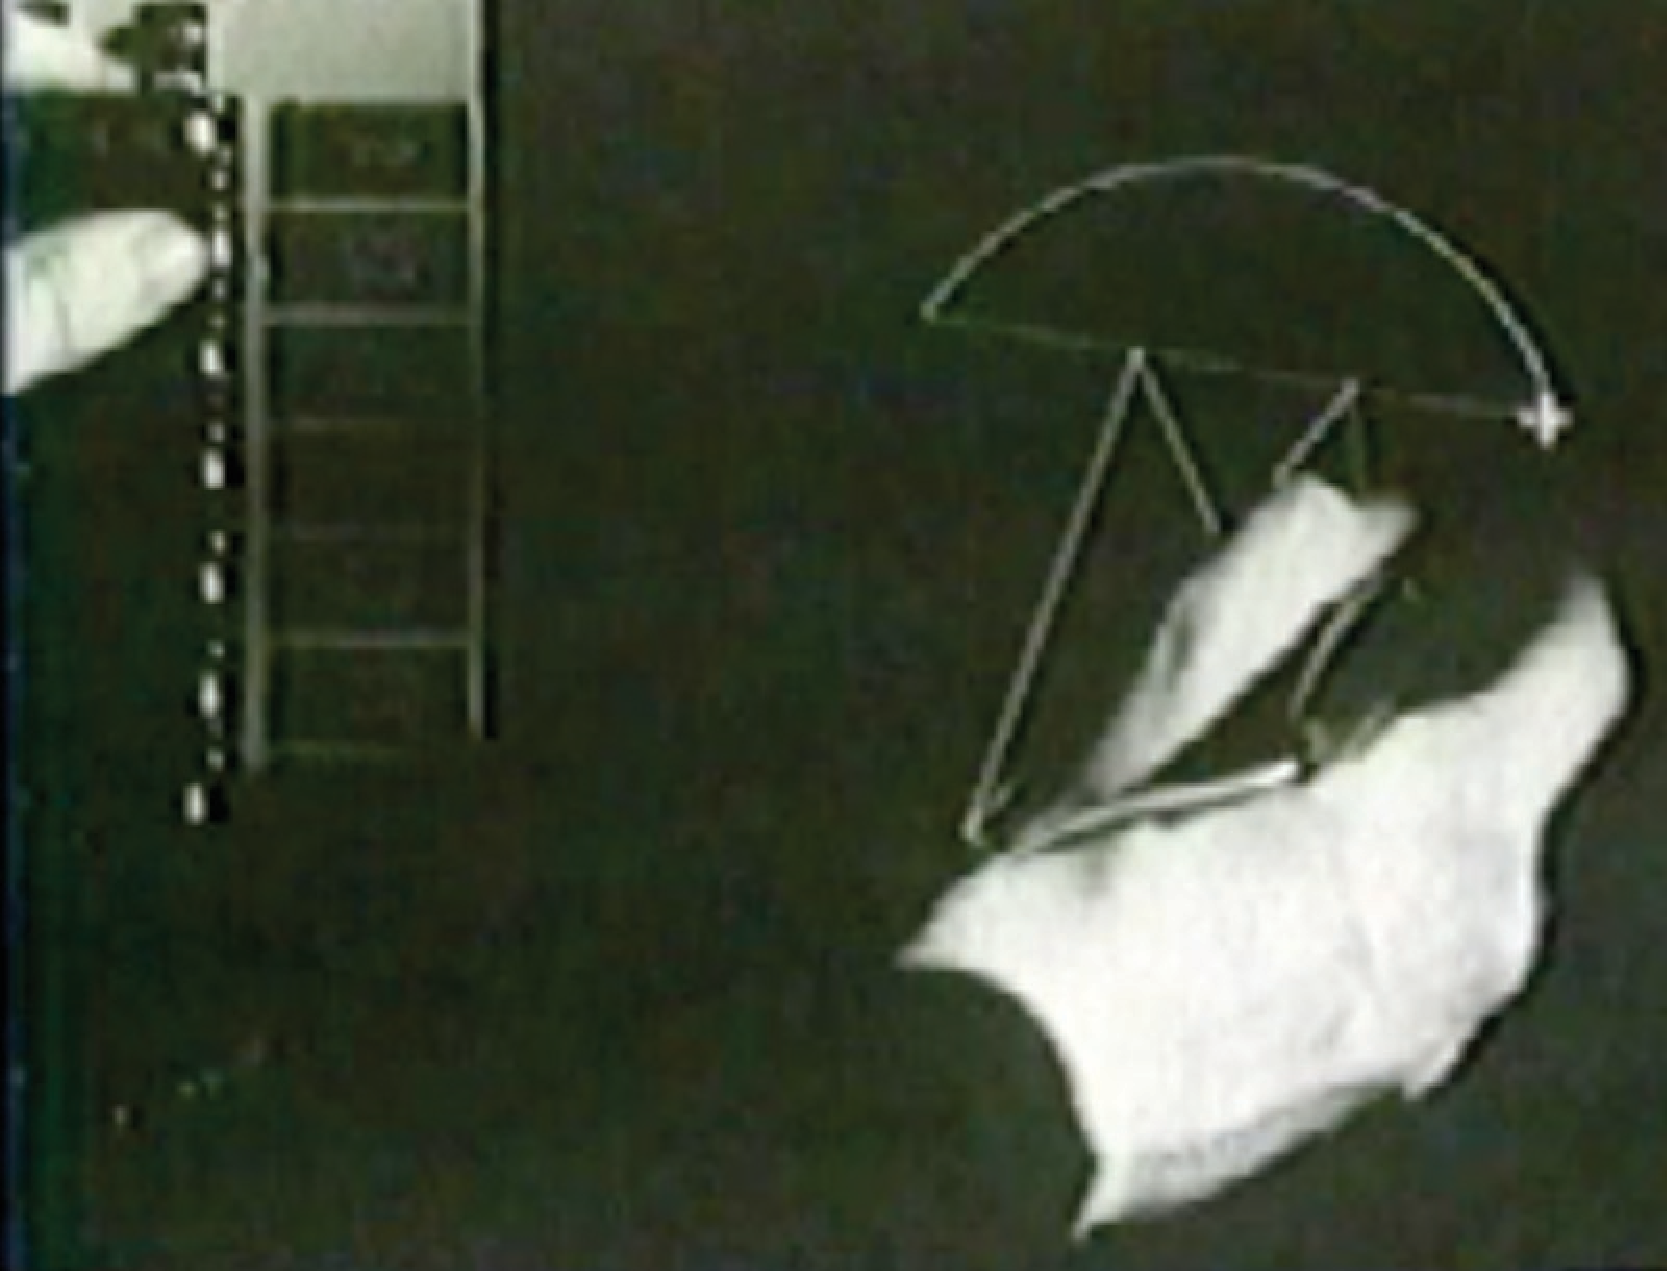
\includegraphics[width=3in]{img/sketchpad.pdf} 
   \caption{Sketchpad supported users in creating design drawings
     using pen input (right hand) and constraints (specified by
     buttons aligned vertically at left).}
   \label{fig:sketchpad}
\end{figure}

Sketchpad was the first to demonstrate many techniques in computer
science, human-computer interaction, and computational
design~\cite{sutherland-sketchpad}. It was an interactive design
system allowing an engineer to create models by drawing with a light
pen on a graphical display. The user could apply constraints (such as
``make this line parallel to that line and maintain that relation'')
that relieved the burden of manually maintaining such
relations. Figure~\ref{fig:sketchpad} shows the user defining the
shape of a rivet through a combination of drawing and constraint
specification.

RAND's GRAIL system (GRAphical Input Language) interpreted stylus
input in a particular visual programming language for creating control
sequence flowcharts~\cite{ellis-grail}. GRAIL allowed users to quickly
specify these programs graphically, rather than textually. To provide
input, users drew or wrote freely on a digitizing tablet. GRAIL then
attempted recognition using domain and contextual information to
determine what the input meant (see Figures~\ref{fig:grail-box} and~\ref{fig:grail-gesture}). The user could add semantically meaningful
model data (boxes, arrows, writing) and issue commands (erase a line,
move a box, change the data type of a node) without explicitly
entering a mode.

\begin{samepage}
\begin{figure}
\begin{center}
  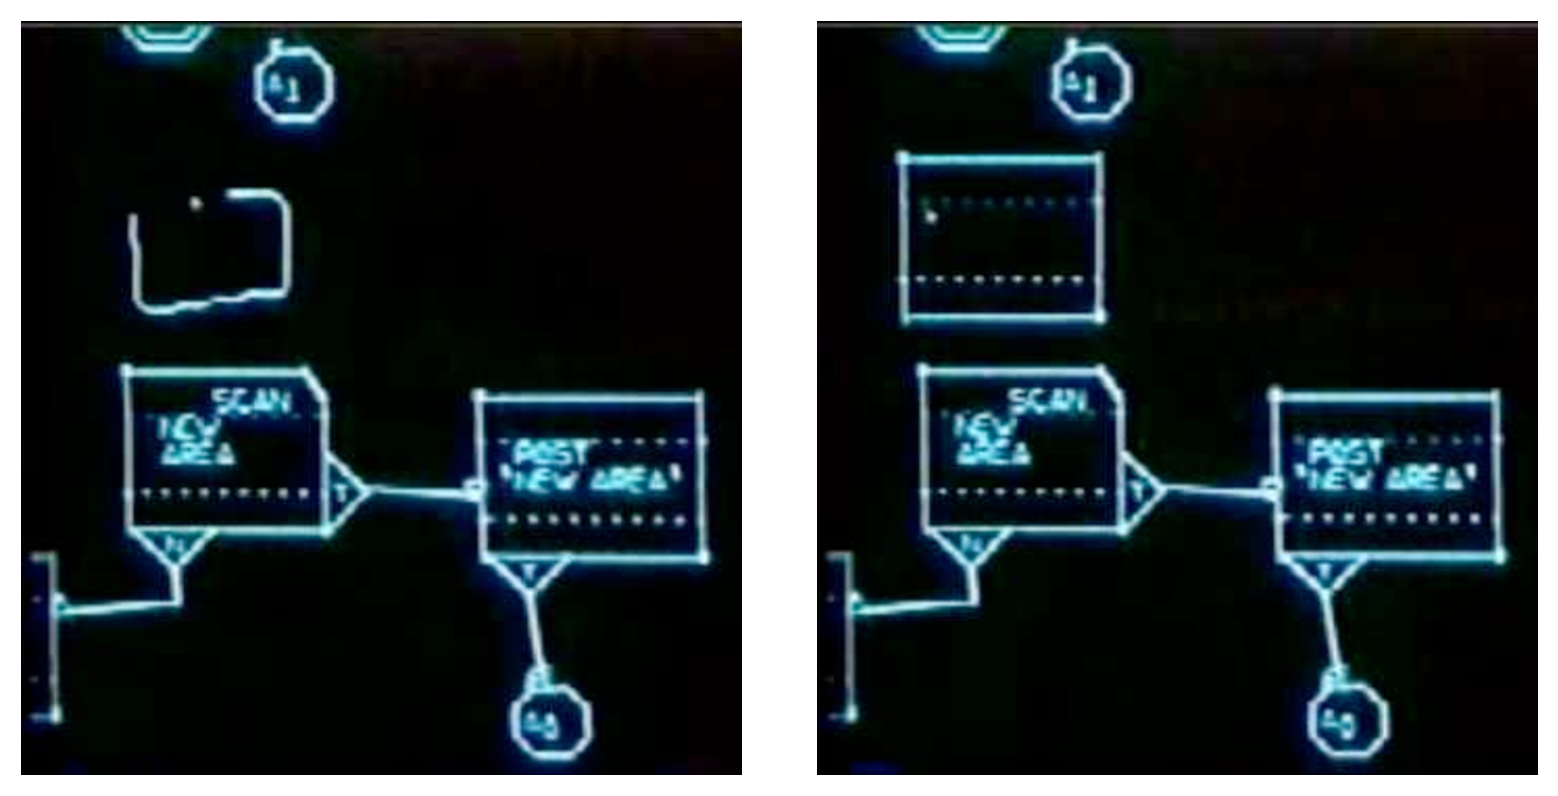
\includegraphics[angle=0, origin=c, width=3.0in]{img/grail-box.pdf} 
  \caption{On left, a GRAIL user draws a model element in place. At
  right, the rectified element is displayed as a box.}
\label{fig:grail-box}
\end{center}
\end{figure}
\begin{figure}
\begin{center}
  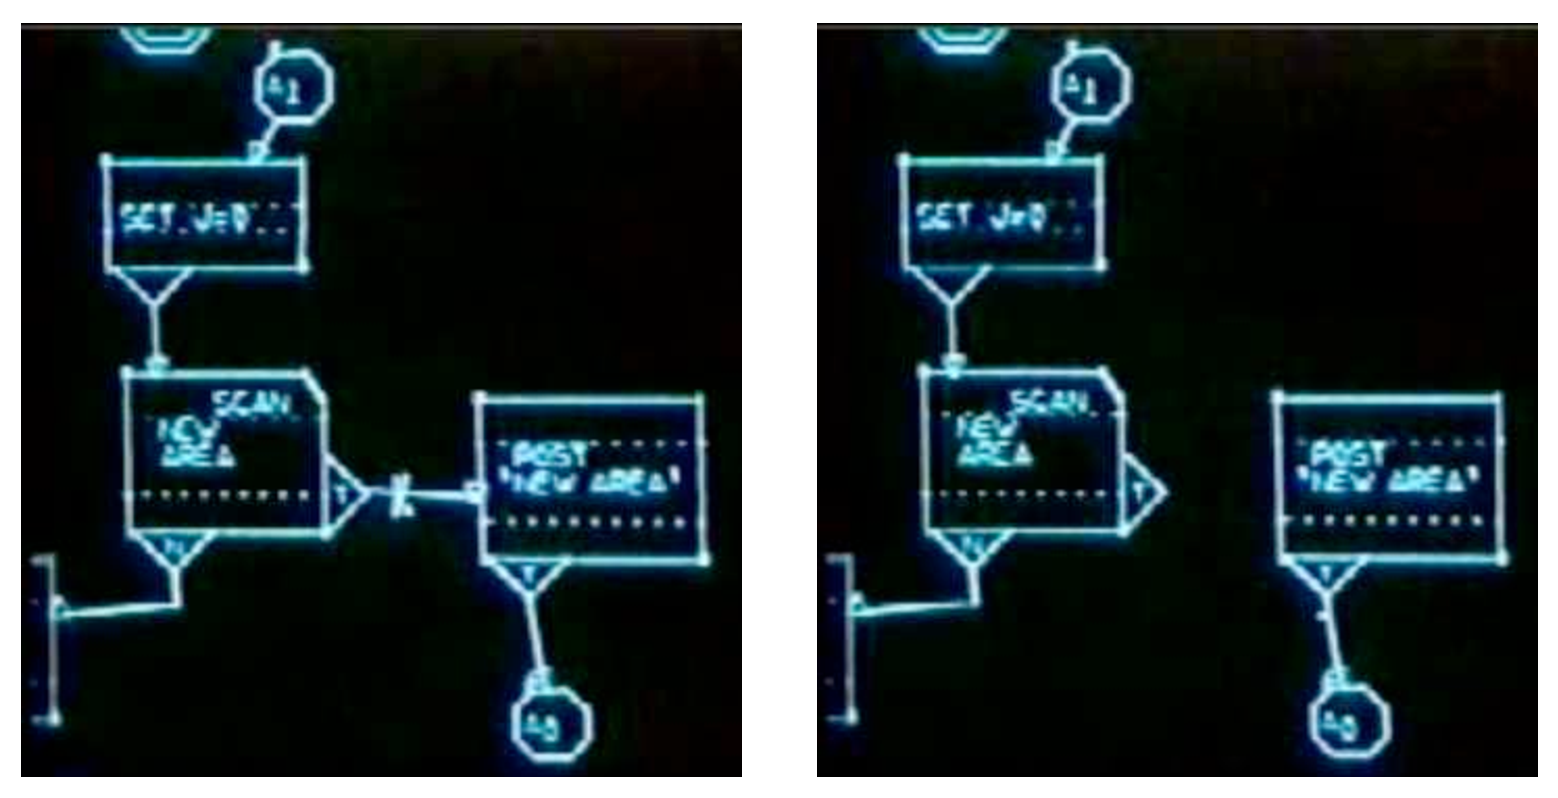
\includegraphics[angle=0, origin=c, width=3.0in]{img/grail-gesture.pdf}
  \caption{GRAIL's sketch interpretation is context sensitive. At left
  the user crosses out the connector, which is interpreted as a delete
  command, shown at right.}
\label{fig:grail-gesture}
\end{center}
\end{figure}
\end{samepage}

Alan Kay discussed Sketchpad and GRAIL in a 1986 lecture. A portion of
that talk is available on the Internet as part of the New Media
Reader~\cite{kay-sketchpad-grail-dynabook,nmr}. Kay shows video of
these pioneering systems and provides insightful commentary, reminding
viewers that much of the work in computer support for sketching has
roots from several decades ago.

There was no widely used pointing device until the Macintosh brought
about the mouse's widespread adoption in the mid-1980s. Owing to the
success of the mouse, pen and sketch based interaction was largely
ignored for years. This began to change when commercial pen computing
products came to market in the early 1990s, bolstered by the prospect
of interaction based on handwriting recognition. Companies such as GO
and GRiD developed and sold pen based tablet devices. IBM's early
ThinkPad computers (700T and 710T) were tablets. Yet these products
fared poorly, and by 1995 many pen computing ventures had gone out of
business. Pen computing did find a niche in the personal digital
assistant (PDA) market with devices such as the Apple Newton and
subsequently the more popular Palm Pilot. However, today's PDAs
typically favor on-screen keyboards over stylus input. Tablet PCs are
currently gaining popularity, primarily for making hand-written notes.

\section{Sketching challenges in HCI}
\label{sec:intro-hci-challenges}

The strength of sketching input lies in the speed and fluidity with
which people can express, interpret, and modify shapes and
relationships among drawn elements without necessarily attending to
details such as alignment or precise measurement. These strengths can
also be seen as the weaknesses of sketching. The equivocal, imprecise
nature of freehand drawing that so benefits humans is exactly why
machines have difficulty recognizing sketches.

Those who aim to create useful and usable systems based on sketch
recognition face a set of challenges including:
 
\begin{itemize}
\item Make hardware to support pen based interaction
\item Build comprehensive, robus toolkits for building sketch based
  systems
\item Create robust sketch recognition algorithms
\item Develop user friendly methods for training and modeling recognizable
 content
\item Design better interaction techniques for sketch based systems
\end{itemize}

This review elaborates on each of these challenges. Progress in one
area will likely require simultaneous work in others. For example, in
order to fully explore interaction design issues in recognition-based
interfaces, we first need sufficiently robust and accurate sketch
recognizers. In order to build recognizers capable of interpreting
sketches made by any person in any domain we must have methods for
modeling domain content. This in turn requires appropriate hardware
and interaction methods.

\section{Research themes in sketch based interaction}

This review details the primary themes of research shown in
Figure~\ref{fig:themes}: support for design, hardware, sketch
recognition, and human-computer interaction techniques. 

\begin{figure}
\begin{center}
  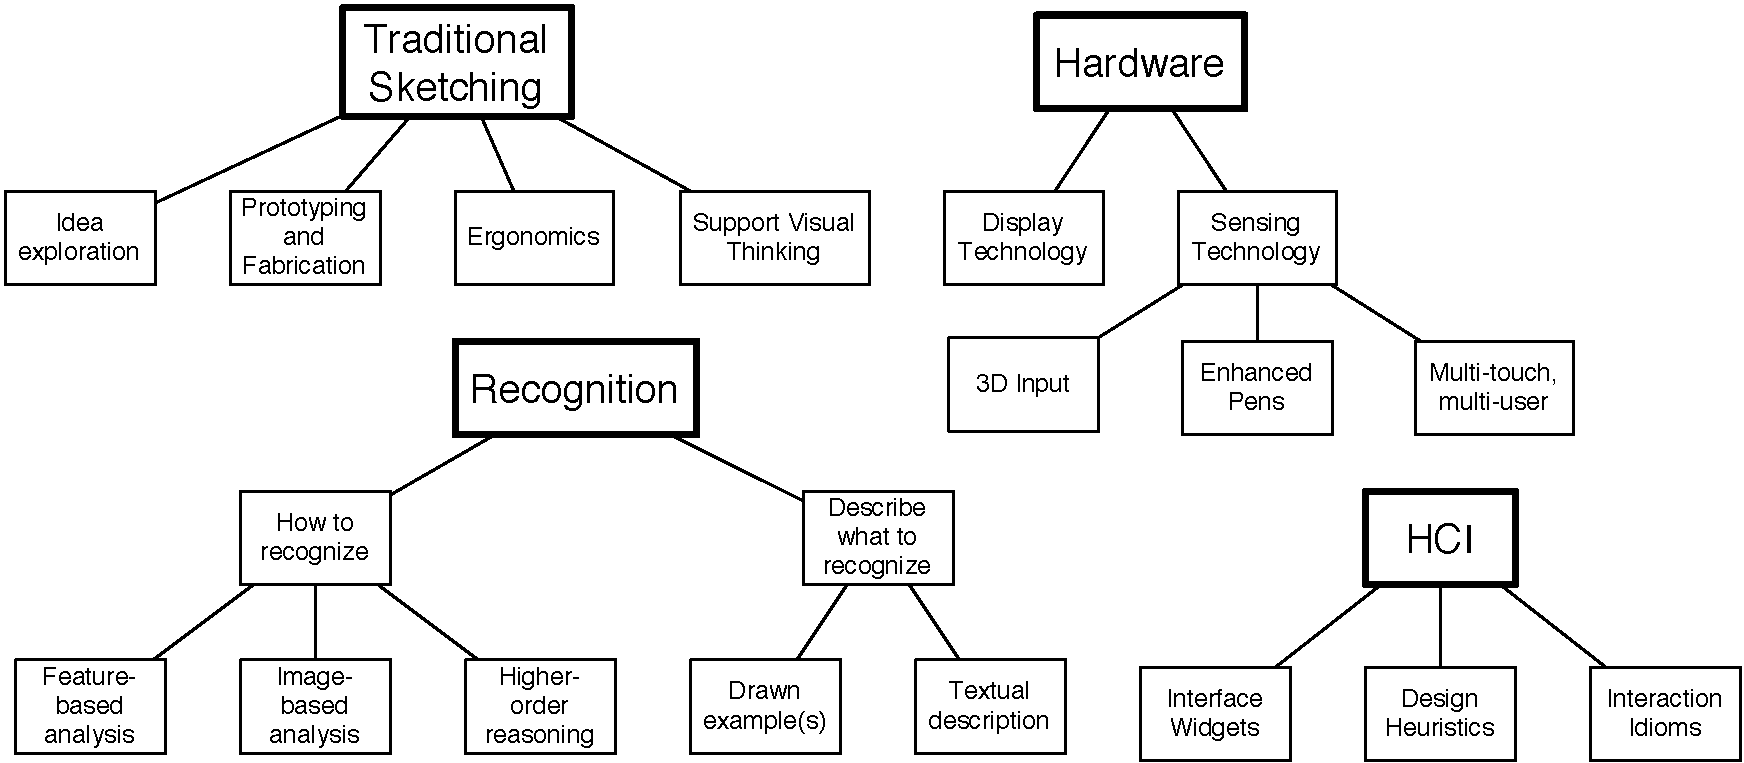
\includegraphics[angle=0,width=\linewidth]{img/themes-3-graffle.pdf}
  \caption{Research themes for sketch based interaction in design}
  \label{fig:themes}
\end{center}
\end{figure}

\textit{Traditional sketching:} (Section~\ref{sec:traditional})
Sketching plays a crucial role in the practice of design.  Sketching
helps designers think about problems and offers an inexpensive but
effective way to communicate ideas to others. The practice of
sketching is nearly ubiquitous: One recent study of interaction
designers and HCI practitioners found that 97\% of those surveyed
began projects by sketching~\cite{myers-behavior-design}. We must
understand the purpose and practice of sketching as it is done
\textit{without} computation if we hope to effectively support it
\textit{with} computation. Most research in computational support for
design sketching has focused on the \textit{early} phases when
designers are exploring high-level ideas. Fewer sketch based design
systems support \textit{later} stages of design when decisions must be
formalized. This section provides a basis for thinking about how, why,
and when (and when not) we may augment sketching with
computation. This discussion covers the cognitive affordances of
sketches and describes several empirical studies.

\textit{Hardware:} (Section~\ref{sec:hardware}) Physical devices
supporting pen based input have existed since RAND's digitizing tablet
was developed in the 1950s. Sensing technology (input) comes in many
forms. Sutherland's Sketchpad system in the early 1960s accepted input
from a light pen~\cite{sutherland-sketchpad}. Some devices promote
using fingers rather than pens, trading accuracy for convenience. Pen
based devices range in size from small (such as PDAs or ``pentop
computers'') to medium (Tablet PCs) to large (electronic
whiteboards). Other hardware considered by sketching researchers
includes electronic paper and ink. The device's size and means for
providing input dictate how and where it may be used, and how mobile
it is. New kinds of devices will lead to new ways of interaction.

\textit{Sketch recognition:} (Section~\ref{sec:recognition})
Recognition is central to many research systems in sketching. For this
reason, a large portion of this review is allocated to discussing
sketch recognition. Some drawn marks indicate domain elements, others
should be taken as commands, while others are annotations. As with
other recognition-based modes of interaction such as speech, sketch
based systems must have a model of what is to be recognized, as well
as algorithms for performing that recognition. Some recognition
techniques rely on input features such as corners, lines, and pen
speed. Other techniques compare the image formed by user input with
known elements. Still other techniques use artificial intelligence
methods such as Bayesian Networks for reasoning about likely sketch
interpretations. To recognize input the system must first have a model
of what may be recognized. Models are frequently made by drawing
examples. Other useful modeling strategies involve textual languages
describing the shape and relationships among visual elements.

\textit{Human-computer interaction:} (Section~\ref{sec:interaction})
User interfaces based on recognizing human speech, gestures, and
sketching pose interesting challenges for researchers in
human-computer interaction. New sketching input hardware, for example,
may promote new interaction styles or allow people to interact with
computers in new contexts, or collaborate in new ways. Because sketch
input may be ambiguous, the interface should not necessarily treat it
in the discrete, deterministic way that mouse and keyboard input is
treated. Further, resolving ambiguity may be delegated to the user,
which requires good interaction design.


\newpage
\chapter{Traditional Sketching}
\label{sec:traditional}

Sketching is the traditional method for early-phase design when both
problems and solutions are unclear. Whereas some might view design as
a process that begins with a fixed problem definition and progresses
by optimization within constraints to refine the problem solution, to
others, the practice of design is as much a matter of
\textit{defining} the problem as \textit{solving} it.

Sketching enables people to work with abstract and uncertain elements,
interpreting and re-interpreting marks on the page that may be
ambiguous or hold alternative contending semantics. Sketched figures,
pictures and maps help people to focus their thoughts or to explain
ideas to others~\cite{do-design-sketches-tools}.

We talk about different kinds of renderings: artistic sketches, study
sketches, drawings, diagrams, schematics, blueprints, and so
on. Although the boundaries are not always clear, each is
characterized by the means of production, the kind of information it
communicates, and the role it plays in problem-solving.

Sketches support quick, informal information processing. We may write
a phone number on the whiteboard near our desk rather than typing. Or,
we may choose to make quick calculations or ``To-Do'' lists on a sheet
of paper because they are portable and easy to make. In his
book \textit{How to Solve It}, George Polya recommends drawing figures
to help understand and solve problems in
mathematics~\cite{polya-solve}. Sketches help us to visualize and
restructure problems to make solutions more readily apparent. For
example, the drawings in Figure \ref{fig:types-of-sketches} were made
by practitioners in different domains. Each depiction helps designers
to think about problems or possible solutions.

There is still a gap between what we know about how and why people
sketch and what kinds of things we can do to support it
computationally. To provide a basis for discussing computational
support we first survey the design and cognitive aspects
of \textit{traditional} sketching done with physical media.

\begin{figure}
\begin{center}

\subfigure[Project management diagram showing task precedence 
           of two projects. Hastily drawn boxes and arrows represent
           abstract activities.]  {

    \label{fig:sketch-type-pm}
    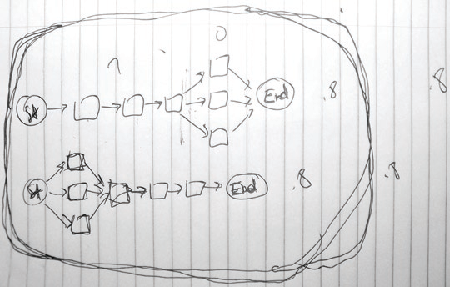
\includegraphics[width=0.42\linewidth]
      {img/sketch-type-project-management.pdf}
}
\hspace{0.03\linewidth}
\subfigure[An architect's floor plan sketch. It includes text, 
           spatial information, and symbols representing household
           items like a piano or dining table.] {

    \label{fig:sketch-type-architecture}
    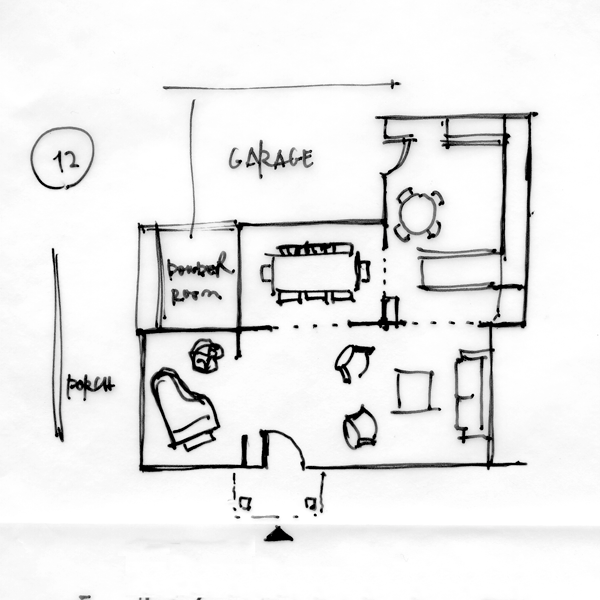
\includegraphics[width=0.42\linewidth]
      {img/sketch-type-architecture.pdf}
}
\caption{Sketches vary in domain and in the visual characteristics of marks.}
\label{fig:types-of-sketches}

\end{center}
\end{figure}

\section{Sketching in design}
\label{sec:traditional-in-design}

While designing, we iteratively explore and refine the problem
definition and proposed solutions. Sketching supports this creative
search process. We set out on our design task with some high-level
goals. However, due to the
ill-structured~\cite{simon-ill-structured-problems} and ``wicked''
nature of design~\cite{rittel-wicked}, we encounter unforeseen
opportunities and constraints as designing progresses. Those
opportunities and constraints may be implicit in the original problem
description, but designers expose them as they explore. The
discoveries are incorporated into the understanding of the problem and
potential solutions. Design problems are ``not the sort of problems or
puzzles that provide all the necessary and sufficient information for
their solution~\cite{cross-nature-nurture}.'' So it goes with
sketching. We draw different views of our model, which allows us to
perceive the problem in new ways.

Designers engage in a sort of ``conversation'' with their sketches in
a tight cycle of drawing, understanding, and
interpreting~\cite{schon-kinds-of-seeing}. Goldschmidt describes this
as switching between two reasoning modes: ``seeing that'' and ``seeing
as''~\cite{goldschmidt-dialectics}. Seeing \textit{that} is the
process of recognizing the literal, descriptive properties of the
drawing.  Seeing \textit{as} is figurative and transformative,
allowing the designer to re-interpret parts of the sketch in different
ways. For example, a designer may draw a sofa and see that the wood
constituting the back rest and the rear supports come into contact. In
this way the designer can see how the two parts could be redesigned as
one. The designer may be able to extract more information from the
sketch than is consciously put into it~\cite{goldschmidt-backtalk}.

Care must be taken to support this reflection when making design
software that employs sketch recognition. If the system interprets
drawings too aggressively or at the wrong time, it may prevent the
human designer from seeing alternative meanings; recognize too little
and the software is no better than paper. This is discussed further in
Sections \ref{sec:recognition-when}
and \ref{sec:recognition-how-much}.

Expertise plays a role in sketching as well. Design students begin to
sketch from the first day. Proficiency in sketching goes beyond
applying marks to the page---one must also interpret and re-interpret
drawings in order to use them effectively. Suwa and Tversky studied
differences between student and professional architects, finding that
professionals had greater skill in transformative
reasoning~\cite{suwa-analysis-students}. Buxton points out the
importance of recognizing the disparity between sketchers who can
expertly \textit{see as} and \textit{see that}, and those who can
not~\cite[page 118]{buxton-sketching}. Trained designers skillfully
examine the content from multiple perspectives, extracting different
interpretations.

Experimental and observational evidence suggest that people of
comparable skill use consistent methods when making drawings. This
consistency applies to the motor action of
drawing~\cite{van-sommers-cognition} and to higher-level semantic
notation. For example, the type of an architectural drawing
(e.g. floor plan, elevation, bubble diagram) can be discerned by
identifying particular visual elements the designer
employs~\cite{neiman-sketch-retrospective,do-design-sketches-tools}.

\section{Prototyping and fidelity}
\label{sec:traditional-prototyping}

Newman and Landay conducted ethnographies of web designers, focusing
on the use of informal design
techniques~\cite{newman-web-designers}. The designers were observed
making models in various media (such as on paper or with a computer)
at various levels of fidelity. Designers always sketch at the
beginning of a web design project, exploring numerous high-level
options. Frequently this early sketching phase is accompanied with
construction of low-fidelity prototypes made on paper or with
Microsoft
PowerPoint\texttrademark~\cite{arnowitz-software-prototyping}. As the
design progresses and designers begin making incremental edits, they
move to higher fidelity models. Client meetings are an important
forcing function in web design projects. When meeting with clients,
designers want to show polished prototypes produced with computer
software. Therefore designers used electronic tools earlier in the
process than they would otherwise have preferred.

Today most software tools support incremental refinement and
specification of details but do not adequately support idea generation
or exploration~\cite{terry-creative-ui}. Designers who begin using
software tools in the early phases of design tend to make superficial
explorations of possible solutions. Further, because tools are poor
for exploration but good for specifying details (font, line weight,
and color), designers tend to focus on nuances that are not yet
important. Observing that current tools are inadequate for creative
pursuits, researchers have developed calligraphic tools such as SILK
and DENIM, which aim to support the early phases of
design~\cite{landay-silk,lin-denim}.

Paper sketches dominate the early phases of design as people generate
new ideas, in a process Goel terms ``lateral
transformations''~\cite{goel-sketches-of-thought}. But as soon as the
web designer believes he or she will make incremental revisions (which
Goel calls ``vertical transformations'') they switch to a computer
tool.

It is not always best to use high-fidelity models for testing
designs. Walker and Takayama observed web site developers performing
usability tests of ongoing interface designs. They found that
high-fidelity, computer-based models are not significantly better than
low-fidelity, paper-based models when testing design
ideas~\cite{walker-fidelity}. This finding supports the conventional
wisdom that inexpensive and quickly made low-fidelity prototypes are
appropriate in iterative design, building, and testing.

\section{Sketches as a symbol system}

\begin{figure}
  \centering
  \subfigure[Overloaded semantics: The cloud and tree have similar
             shapes but different meanings due to context.] {
    \label{fig:cloud-1} 
    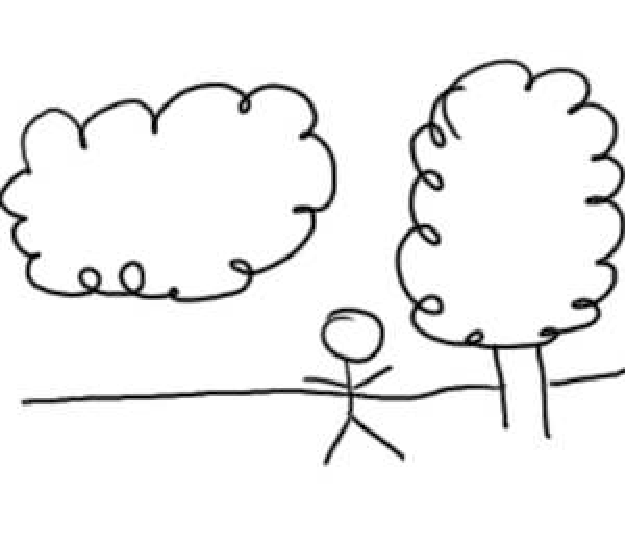
\includegraphics[width=0.25\linewidth]{img/cloud-1.pdf} 
  }
  \hspace{0.03\linewidth}
  \subfigure[Ambiguity: Changing the drawing slightly changes our
             interpretation. The object on the left may be a cloud, or
             it may be a cartoon thought bubble.] { 
    \label{fig:cloud-2} 
    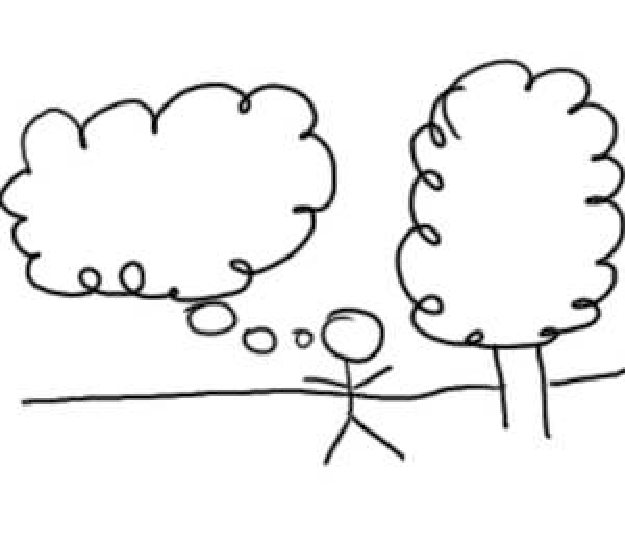
\includegraphics[width=0.25\linewidth]{img/cloud-2.pdf} 
  }
  \hspace{0.03\linewidth}
  \subfigure[Additional information helps us reason about the intended
             identity of elements. Text inside the cloud indicates it
             is a cartoon thought bubble.]  {
    \label{fig:cloud-3} 
    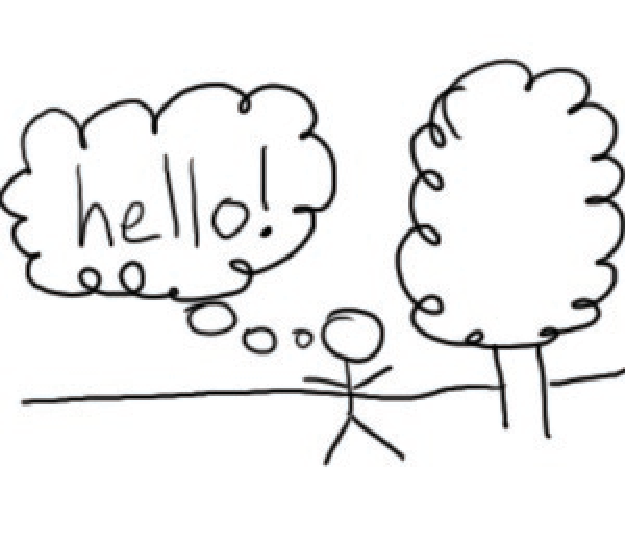
\includegraphics[width=0.25\linewidth]{img/cloud-3.pdf} 
  }
  \caption{Overloaded semantics and ambiguity.}
  \label{fig:cloud}
\end{figure}

Goodman provides a comprehensive framework for analyzing the
properties of various symbol systems, including
sketches~\cite{goodman-symbols}. Goel places sketching in Goodman's
framework, noting that sketches have \textit{overloaded semantics},
they are \textit{ambiguous}, \textit{dense},
and \textit{replete}~\cite{goel-sketches-of-thought}. These properties
describe one particular sense of sketching in which the drawer's marks
may be idiosyncratic.

Sketches have ``overloaded semantics'': The same symbol may mean
different things depending on context. Further, a sketched symbol may
be ``ambiguous'', meaning that the symbol affords more than one
plausible interpretation.  Figure~\ref{fig:cloud} illustrates these
properties. A lumpy shape can be used to indicate many things
including clouds, trees, or thought bubbles. We interpret the shape
differently depending on context.

Sketched symbols are ``dense'', indicating there is a continuous range
between instances of the same symbol. While there may be minute visual
discrepancies between symbol instances, Goel claims that such symbols
are also ``replete'': no aspect of the sketched symbol may be safely
ignored (Figure~\ref{fig:dense-replete}).

The pen strokes constituting a sketch serve various functions. Ink may
indicate abstract domain symbols (e.g. diode, treble clef), object
boundaries, actions (e.g. arrows indicating containment or movement),
dimensions and units, annotations, region texturing, and so on. Some
parts of a sketch are more dense and replete than others. For example
a diode's properties do not change if it is drawn with a slightly
larger triangle. However, subtle variations in how a desk lamp is
drawn might lead to substantially different aesthetic responses to it.

\begin{figure}
\begin{center}
  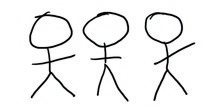
\includegraphics[angle=0, origin=c,
  width=3.5cm]{img/dense-replete-stick-figures.pdf}

  \caption{Different instances of the same stick figure vary along a
  continuum (\textit{dense}). However, the visual properties of
  individual symbols may (or may not) communicate additional
  information (\textit{replete}). Is the figure at the right waving? }

  \label{fig:dense-replete}
\end{center}
\end{figure}

Gross and Do discuss some properties of hand-drawn diagrams from the
perspective of building tools to support design drawing
activities~\cite{gross-ecn-uist}. The authors distinguish sketches
from diagrams, noting that diagrams are ``composed of primitive
elements chosen from a small universe of simple symbols---boxes,
circles, blobs, lines, arrows.'' This list is certainly not
exhaustive, but it does illustrate the general idea that diagrams have
a limited vocabulary. In practice, sketches and diagrams from various
dialects may be combined (e.g. mathematical notation on the same page
as circuit diagrams and hand written notes.)

Freehand diagrammatic drawings are abstract, ambiguous, and
imprecise. \textit{Abstract} symbols denote elements whose identities
or properties are not (yet) important or known. For example,
Figure~\ref{fig:sketch-type-pm} on page \pageref{fig:sketch-type-pm}
shows a project management diagram of two hypothetical projects. The
activities composing each project are abstract---they could represent
anything. The value of the sketch is that it shows the project's
network topology and does not draw attention to what the specific
activities are. 

An \textit{ambiguous} symbol has many plausible interpretations. The
floor plan sketch in Figure~\ref{fig:sketch-type-architecture} shows
several rectangles indicating rooms, furniture, shelves, or
counters. Human observers can confidently disambiguate the intended
meaning of some rectangles, but others remain unclear. The
bottom-right of the sketch shows two armchairs and a sofa with an
ambiguous rectangle in the middle that could plausibly represent
either a rug or a coffee table.

Last, freehand diagrams are \textit{imprecise}. Imprecision allows
designers to work with rough values (e.g. ``about two meters wide'')
and avoid premature commitment. Imprecision also indicates that the
design is by no means final.

The notational properties of sketches make them powerful tools for
supporting visual thinking. Designers may leverage ambiguities in
their sketches to see new meanings, for example. However, these same
properties present challenges for accurate software recognition.

The degree to which a drawing is ambiguous, imprecise, and abstract
varies among instances, and people might interpret them differently. A
rough sketch is useful to designers, especially for brainstorming and
incremental development of ideas. But in order for the sketch to be
transformed into a finished product (e.g. for manufacturing), it must
be made unequivocal, precise, and concrete. The process of moving from
the informal sketch to the formal specification involves drawings that
are semi-ambiguous, partially precise, and with some abstractions
given definite identities.

\section{Cognitive and mechanical aspects of drawing}
\label{sec:traditional-cognitive-mechanical}

Larkin and Simon compared \textit{diagrammatic} notation
with \textit{sentential} (written or spoken) systems, suggesting that
spatial notation often affords more efficient information processing
than an equivalent written
statement~\cite{larkin-diagrams}. \textit{Efficiency} of information
processing refers to how much computation is necessary to translate
input into understanding. For example, we may state the relationship
between supply and demand in a market economy with a mathematical
(sentential) description as in
Figure~\ref{fig:markets-sentential}. Market equilibrium is found where
the values of supply and demand intersect. In a sentential
representation, we must calculate to find equilibrium. However, given
a graph (diagrammatic) as in Figure~\ref{fig:markets-diagrammatic}, we
directly see where the supply and demand curves intersect and
immediately read the associated values. Even though the
representations provide equivalent information, the diagrammatic form
can be more efficient, depending on the viewer's goals.

\begin{figure}
  \centering
  \subfigure[Written (sentential) form.] { 
    \label{fig:markets-sentential} 
    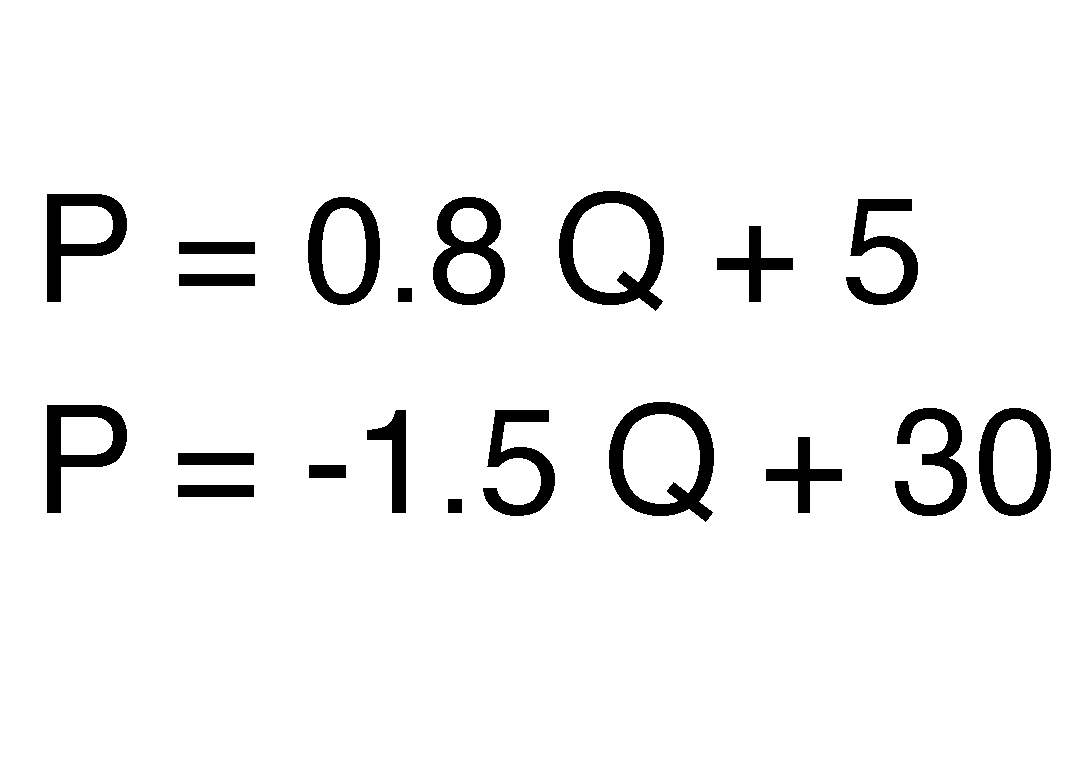
\includegraphics[width=2in]{img/market-eqn.pdf} 
  }
  \hspace{0.5cm}
  \subfigure[Graphic (diagrammatic) form.] {
    \label{fig:markets-diagrammatic} 
    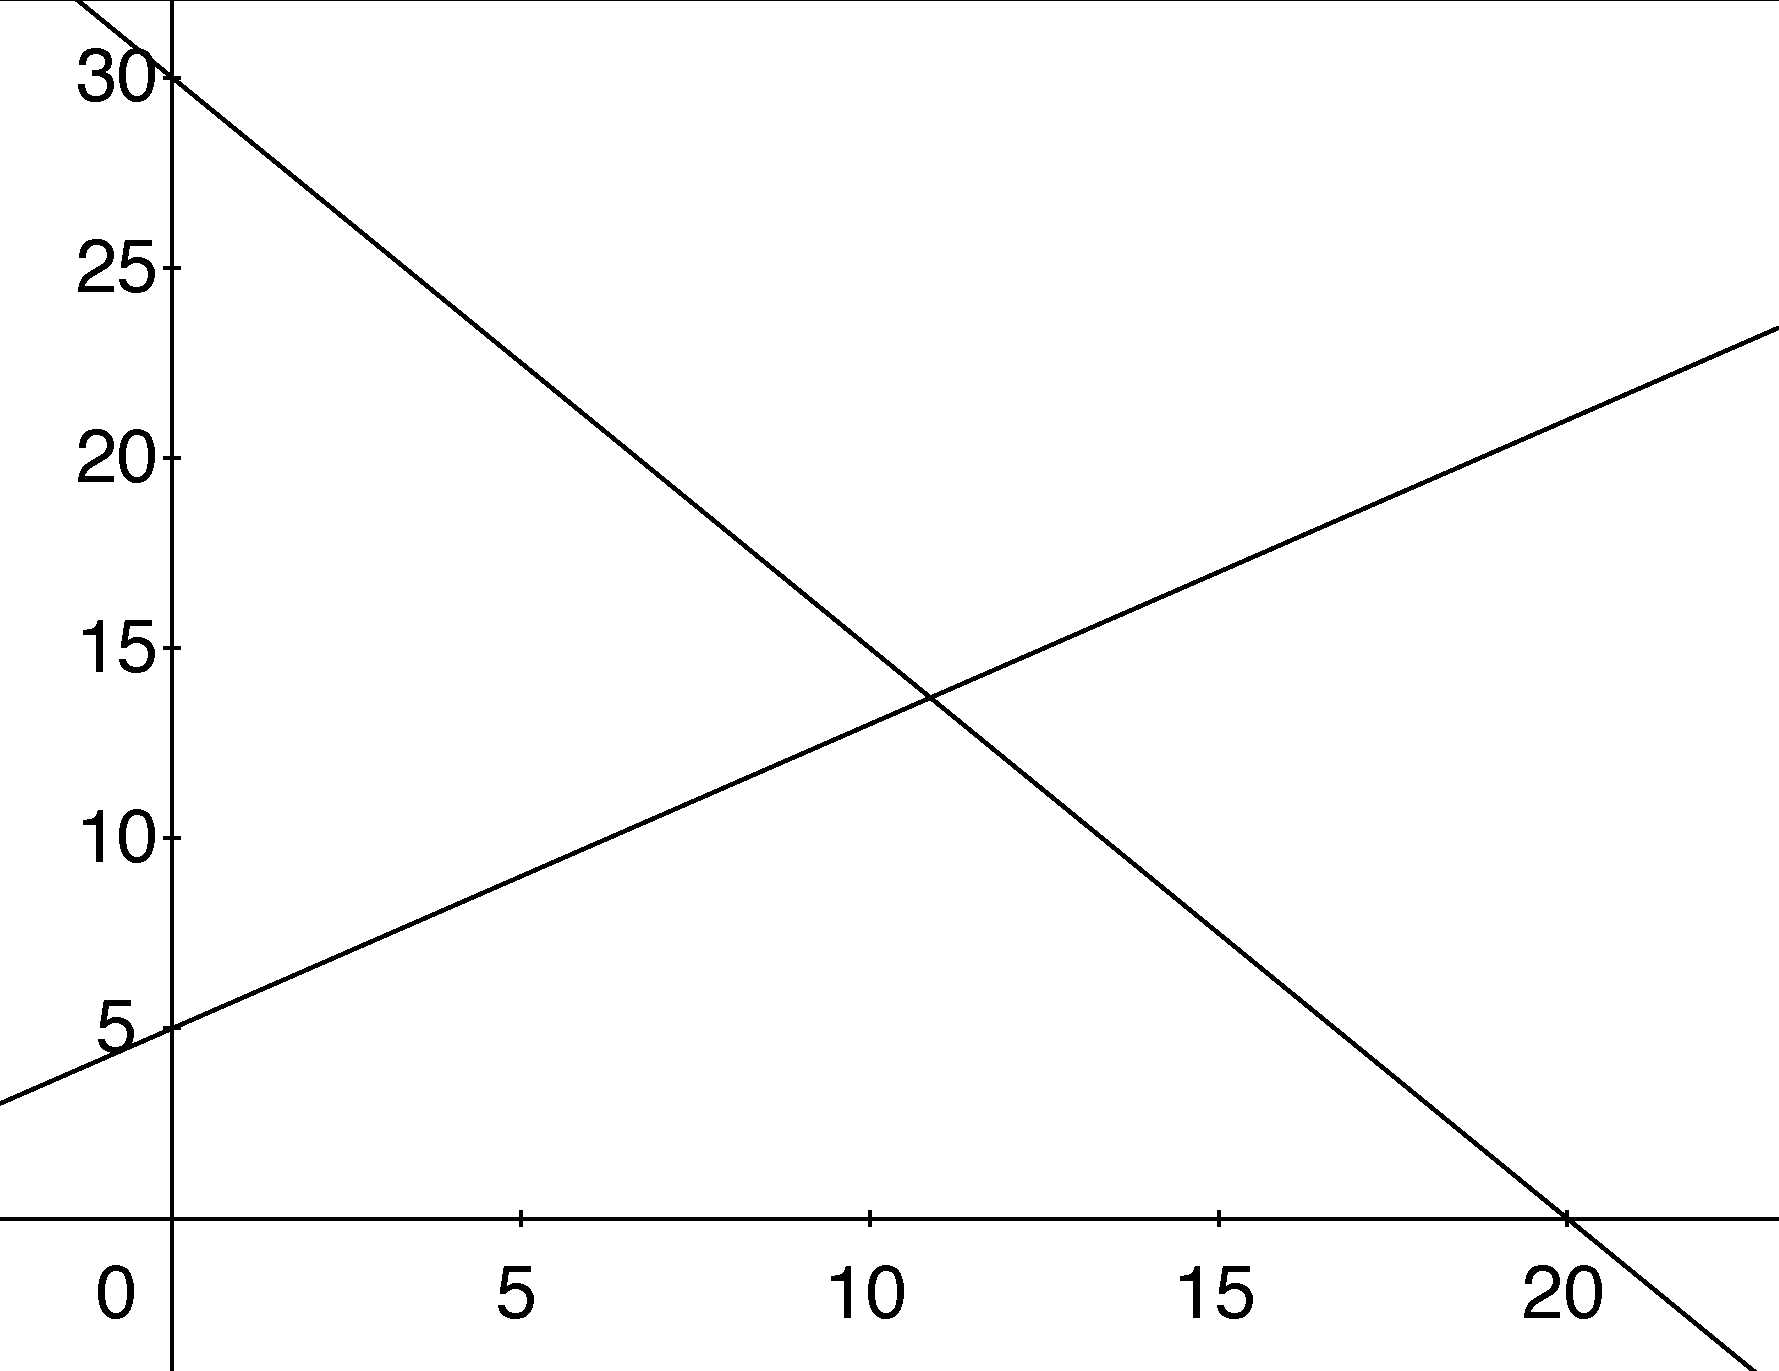
\includegraphics[width=2in]{img/market-graph.pdf}
  }
  \caption{Sentential and diagrammatic representations of supply and
  demand provide equivalent information.}
  \label{fig:markets}
\end{figure}

When people sketch, they ``incorporate relevant information and omit
the irrelevant''~\cite{tversky-sketching-thinking}. Drawing allows
people to use paper as external storage, reducing and augmenting
cognitive load. Diagrammatic notation schematizes domain
information~\cite{tversky-diagrammatic-communication}. Hand-drawn
route maps, for example, are usually made with a simple visual
vocabulary consisting of rectangles or circles indicating buildings,
lines or arcs representing paths, and junctions where paths
intersect~\cite{tversky-routes}. The shape and curvature of buildings
and paths is drawn approximately. Given a well-drawn map, humans have
little trouble reconciling differences between the map and the
physical world it represents.

Spatial representations offer a powerful means for learning in many
domains. Sketching allows learners to represent concepts as they
understand them, and allows more experienced people to spot
inconsistencies or areas where additional learning is
needed~\cite{forbus-cogsketch-tutorial}.

Van Sommers extensively studied how people
draw~\cite{van-sommers-cognition}. This includes the mechanics of
using one's arm, wrist, hand, and fingers when drawing. His research
examines the effects of culture, handedness, and expertise on how
drawings are made. He found that of the many possible ways of making a
drawing, subjects tended to use consistent strategies. For example,
subjects were asked to trace over short lines scattered about a large
sheet of paper. The lines did not overlap and represented the full
range of rotations. Right-handed drawers had a strong tendency to draw
from left to right and top to bottom. Left-handers also showed the
tendency to draw top to bottom but showed a slight preference towards
drawing right to left.

Sezgin gives a compelling example of consistent stroke
ordering~\cite{sezgin-phd-thesis}. Participants were asked to draw
common objects such as the stick figure shown in
Figure~\ref{fig:stick-figure} thirty or more times. This stick figure
has six components: the head, a torso, two arms, two legs. The lines
can be drawn in 720 distinct sequences \nohyphens{($6!=720$)}.
However, participants used only about five of those component
orderings to draw the figure. Further, each participant showed a
strong individual bias to draw the symbol using the same sequence
(e.g. head, torso, legs, and finally the arms).

\begin{figure}
\begin{center}
  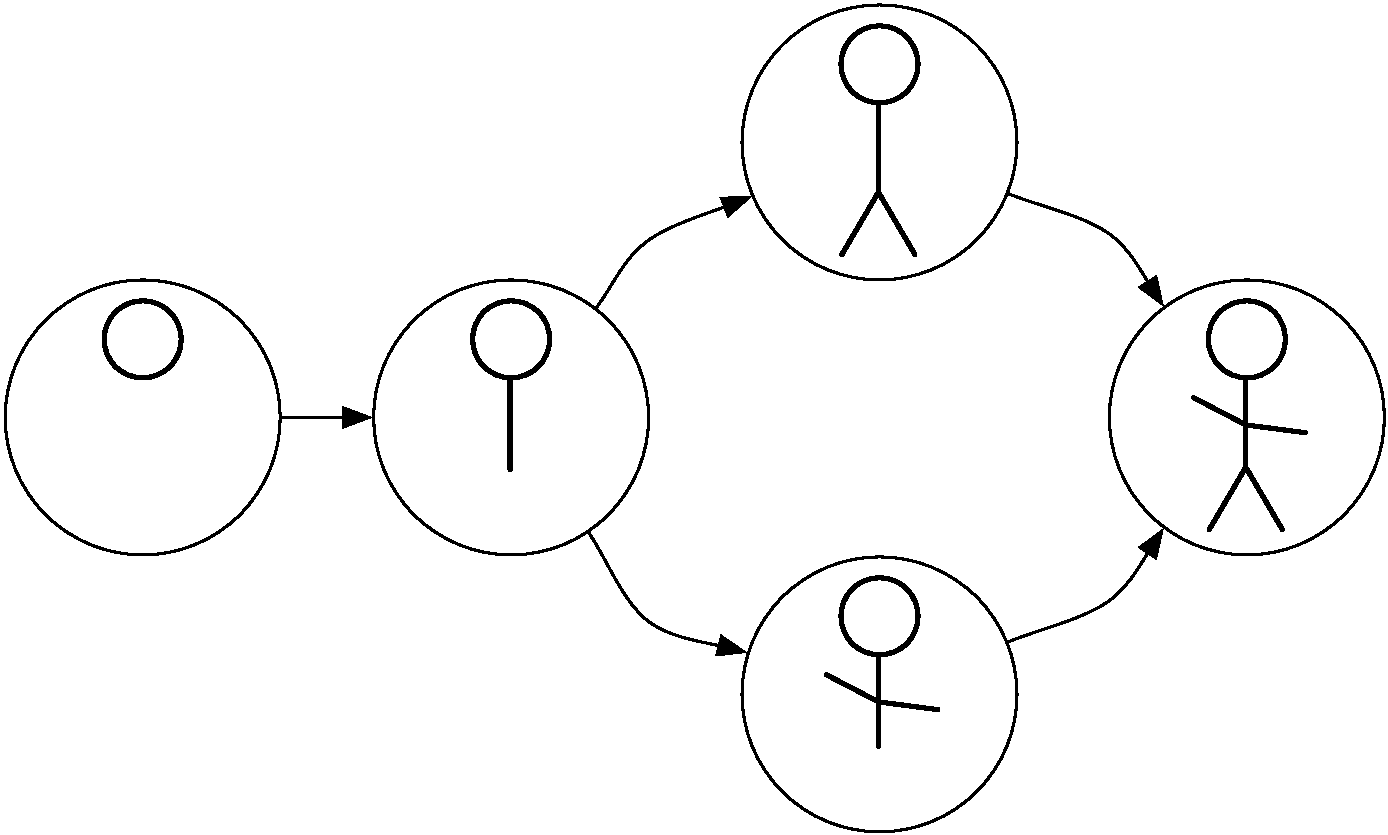
\includegraphics[width=2.5in]{img/sezgin-sketching-style-diagram.pdf} 

  \caption{A stick figure with six components can be drawn in any one
  of 720 possible orders, but only about five are used in
  practice \protect~\cite{sezgin-phd-thesis}. Two of those orders are
  shown in this sketching style diagram.}

\label{fig:stick-figure}
\end{center}
\end{figure}

A drawer's preferred direction of making strokes depends on the
semantics of whatever is being drawn. Van Sommers shows that although
people will choose to draw arbitrary lines according to a preference
(largely determined by handedness), people will deviate from those
preferences when drawing things that hold meaning. Participants were
asked to draw common things, including a rake and cigarette smoke. We
know from experience that a rake is held at the top with the rake's
fingers contacting the ground. Cigarette smoke rises. Van Sommers'
participants generally drew the rake from top to bottom, but the smoke
from bottom to top. He posits this is because our knowledge of an
object's properties informs the way we draw it.

Stroke ordering can also be affected by perceptual properties of a
drawing, even if the drawing's meaning is not clear.  Van Sommers
asked experiment participants to trace over the picture in
Figure~\ref{fig:grape-clusters}. Each ``grape'' in a cluster has a
boundary. The number represents the mean position in the drawing
sequence. The grape ``on top'' is usually drawn first, with
neighboring grapes drawn next.

Van Sommers uses the term \textit{anchoring} to explain the sequence
that some strokes are made. Anchoring is an example of a control
strategy for making marks. The grape ``on top'' serves as a convenient
anchor for drawing its neighbors. It is easier to control the start
and end locations of a mark if there is already something to attach it
to. Another control strategy for making marks
is \textit{containment}. In depictions with a structure enclosing
something else (such as a bowl of fruit), the container is typically
drawn first. Anchoring and containment may be useful control
strategies for improving sketch recognition efficiency.

\begin{figure}
  \begin{center}
  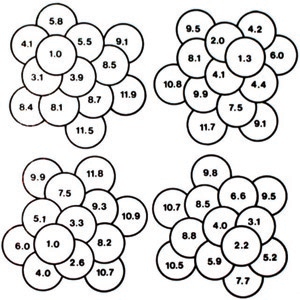
\includegraphics[width=2in]{img/van-sommers-grapes.pdf}
  \caption{``Grape Clusters'' drawn by right-handed participants in
    van Sommers' study showing the mean position in the drawing
    sequence.}
  \label{fig:grape-clusters} 
  \end{center}
\end{figure}

Some researchers have noted the prominent place of sketching in design
and have studied sketching as a tool. A series of experiments by Goel
looked at the cognitive affordances of
sketching~\cite{goel-sketches-of-thought}. These studies compared
traditional pencil-and-paper sketching with sketches made with a
computer drawing application. Participating designers were asked to
design an artifact using either a software paint program or using
pencil and paper. The software tool was modified to only support
structured input such as straight lines, rectangles, and ellipses. He
found that the structured notation system (computer application) did
not afford the same level of rapid exploration of design ideas as
using an unstructured system (pencil-and-paper freehand
sketching). Sketching supports designers in easily trying many ideas,
which Goel calls \textit{lateral transformations}. This is
distinguished from \textit{vertical transformations}, characterized by
refining ideas rather than exploring new ones.

The transformation types identified by Goel correspond to the
activities done at different stages of design described by Newman and
Landay~\cite{newman-web-designers}. Early in the design process
designers are concerned with idea generation and exploration (lateral
transformations). Later on designers make iterative revisions and
refinement (vertical transformations). The goal of many computational
sketching tools is to support lateral transformations.


\section{Summary: traditional sketching and computation}
\label{ref:traditional-summary}

If we hope to effectively support sketching with computation, we must
first understand the practical aspects of traditional sketching. 

Sketching is an important---perhaps necessary---tool for doing
design. It gives us a way to quickly make provisional drawings, which
help us efficiently make sense of spatial, relational
information. Sketches let us make marks that are as vague or specific
as we need. Because sketched elements can easily be ambiguous, rough
drawings afford different interpretations. We may therefore reflect on
our sketches and see new meaning in existing marks. People sketch in
part because they don't know exactly what they are making---sketching
facilitates exploration.

Low-fidelity prototypes are especially important as tools to test
ideas during early design. This is because they are easy to make,
allowing designers to quickly expose problems before committing to
decisions. Sketching is a common method of creating such prototypes.

In order for computers to recognize sketches, we must develop
techniques to transform imprecisely made marks into discrete
symbols. However, some of the properties that make a sketch useful for
a human (overloaded semantics, ambiguous, imprecise, etc.) complicate
the task of computer recognition.

We can make use of consistencies in how people draw to inform
recognition. First, we observe that some kinds of sketches are made
using restricted visual vocabulary, e.g., diagrams of electronic
circuits or web page layouts. Second, consistencies in the mechanical
act of drawing (such as anchoring and containment) can be used to
further guide recognition. For example, recalling
Figure~\ref{fig:stick-figure} we know that people are likely to use
only a small number of ways to draw a stick figure even though there
are hundreds of possible stroke orderings. This can help make
recognition strategies more efficient by utilizing commonly used
patterns before less frequently used ones.


\newpage
\chapter{Hardware Support for Sketching}
\label{sec:hardware}

Today's pen hardware is largely oriented towards reading and writing
text. However when considering hardware support for design activities,
we may compare current computational hardware with the physical
artifacts designers use in practice. Designers can quickly draw on
sheets of paper, and flip through them easily. Or we might pin the
papers next to each other on a wall to compare and contrast ideas. The
tip of the pen instantly deposits as we draw exactly where we have
made contact with the page. We can use two hands to rotate the paper
to a desired angle or use secondary devices such as a straight edge in
aid of careful drawing.

It would be simplistic to argue that computational support for
sketching should exactly mimic practices supported by physical media.
However, current hardware lacks the portability, responsiveness, and
feel of tools of traditional design practice. Commercial development
and research continue to improve hardware support in these categories.

Many devices such as PDAs, tablet-style computers, and wall-size
interactive screens feature some kind of pen (stylus) or touch
input. While pen based systems have been available to researchers for
decades, only since the mid-1990s have systems become inexpensive and
common.

Hardware for sketching can be separated into two groups: those that
support input only, and those that support input and output.

Some digitizing tablets afford input by letting people write or draw
with a stylus. These are not output devices---they do not display the
user's marks. Sketches are also input by scanning drawings. For
example, PARC's research system ScanScribe analyzes marks made with
everyday pen and paper to produce a computationally enhanced version
of the drawing~\cite{saund-scanscribe}. It is common for a single
device to provide both input and output where the drawing surface is
the same as the display surface, as exemplified by Tablet PCs.

Here we consider hardware that is appropriate for use in sketch based
interactive systems. This hardware ranges from small (pen computers,
PDAs) to medium (tablets, desktop workstations) to large (table top or
whiteboard systems). 

\section{Computationally enhanced pens and paper}

We begin our discussion of sketching hardware with commercially
available devices such as the Anoto Pen~\cite{anoto}. They are
slightly larger than ordinary pens, but small and light enough to use
like any other pen. They mark the paper with ink, letting users keep a
paper record of their use. Pen activity can be transmitted as it is
used, or stored for later use.

The Anoto Pen is used on special paper featuring a pattern of tiny
dots. Each sheet has a unique pattern. A small infrared
camera monitors a region near the pen's tip. Firmware decodes the
local pattern of dots and determines where the user is marking.

Device producers have licensed Anoto's technology and produced their
own pens, such as Logitech's io2 or LeapFrog's Fly pen. The Fly
recognizes a limited set of user actions and provides audio feedback
with a small speaker housed inside the pen. For example, the user can
draw a simple calculator on Anoto paper and then use it to perform
basic arithmetic. The pen speaks the calculations it makes.

Paper Augmented Digital Documents (PADD) are a class of ``digital
documents which one can manipulate either electronically or on
paper''~\cite{guimbretiere-padd}. It provides ways to bridge the gap
between virtual and physical paper. For example, ModelCraft enables
users to manipulate electronic 3D models using paper as the input
device~\cite{song-modelcraft}. PaperPoint allows control and
annotation of PowerPoint presentations using printed copies of slides
~\cite{signer-paperpoint}. West \textit{et al.} describe their
Anoto-based MEMENTO system that elders use to create digital
scrapbooks using paper~\cite{west-memento}. MEMENTO and PapierCraft
and other augmented paper technologies leverage the convivial,
easy-to-use aspects of pen-and-paper while enabling people to easily
manipulate virtual artifacts.

Another enhanced ink pen device was the CrossPad, sold from 1998 to
2001~\cite{crosspad}. It allowed users to write on a traditional pad
of paper using an ink pen. The pen's location was calculated by a
receiver clamped to the writing pad. Ink data could later be
transferred to a PC, which performed handwriting recognition.

\section{Input surfaces and styluses}
\label{sec:multi-sense}

Many digitizing tablets sense
pressure~\cite{meyer-pen-review}. Designers often use heavier lines to
indicate object boundaries, and lighter lines to indicate subtle (but
potentially important) texturing, shading, or curvature. Devices that
sense pressure can allow designers to create thicker or darker lines
without changing drawing tool modes.

Pressure sensing has been implemented in a number of ways, for
example, two conductive layers with current flowing in orthogonal
directions. The layers do not touch and may be separated with a
non-conductive layer of fluid. When something (a pen, a finger)
contacts the upper surface, voltage changes are measured at layer
edges. The contact location is calculated by interpolation. Other
touch surfaces sense electrical properties of things contacting
them---this is why a gloved finger will not work on many laptop
trackpads. Wacom\texttrademark\ tablets and similar inductive devices
depend on a special stylus that resonates in an electromagnetic field
generated by the tablet surface. Still other tablets detect
acoustic~\cite{debruyne-acoustic} or optical disturbances for
calculating input position.

Some sensing surfaces report a single location of contact, but
multi-touch surfaces identify more than one input coordinate. Recent
multi-touch systems have become popular, including Han's Frustrated
Total Internal Reflection technique~\cite{han-multitouch} and
Microsoft's Surface system~\cite{microsoft-surface}. MERL's
DiamondTouch is a multi-touch tabletop display that also supports
multi-user interaction. DiamondTouch discerns individual users based
on different capacitance levels as the user completes a circuit
between the surface and a pad placed on their chair. 

Input surfaces that are intended to be used with fingers or hands
offer different interaction experiences than pen-oriented drawing
surfaces. For example, users may trace shapes with a single finger,
use two fingers to zoom in or out, or use whole-hand gestures for
issuing other commands. These interaction techniques may provide
opportunities for developing innovative sketching applications.

\section{Distinction between pen and mouse}
\label{sec:computation-pen-vs-mouse}

Regardless of sensing technology, all these devices allow users to
provide input in a way that is much closer to traditional writing than
a mouse allows. Although pen and mouse input share many properties
(both allow users to interact with 2D displays) they have several key
differences.

Mouse input affords \textit{motion} sensing while pen input
affords \textit{position} sensing~\cite{hinckley-input-technology}. In
other words, while mice produce the relative \textit{change} in
$(x,y)$ locations, pens directly provide absolute $(x,y)$ locations.
Users can configure tablets to report relative position, thereby
behaving like a mouse.

Form is also extremely important. A stylus affords people to use the
fine motor abilities of their fingers to control the tip of the pen,
whereas hand and forearm muscles dominate mouse usage. Fingers can be
used to move the mouse, but not with the same dexterity possible with
a pen. Depending on the type of work, a pen may be ergonomically
superior to a mouse, or the other way around.

Digitizing tablets can detect more than the stylus position. Some
devices sense stylus pressure, its angle relative to the tablet, or
its rotation. The non-writing end of the stylus is sometimes used as
an alternate tool mode (e.g. as an eraser).

\begin{figure}
\centering 

\subfigure[Pressing a mouse button exerts force perpendicular to the
  operating plane.] { 
  \label{fig:button-force-mouse} 
  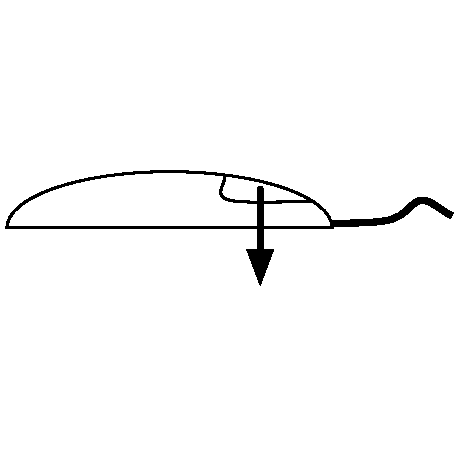
\includegraphics[origin=c, width=3.5cm]{img/button-force-mouse.pdf} 
}
\hspace{1cm} \subfigure[Pressing a stylus button is likely to cause
  accidental pen tip movement.] {
    \label{fig:button-force-pen}
    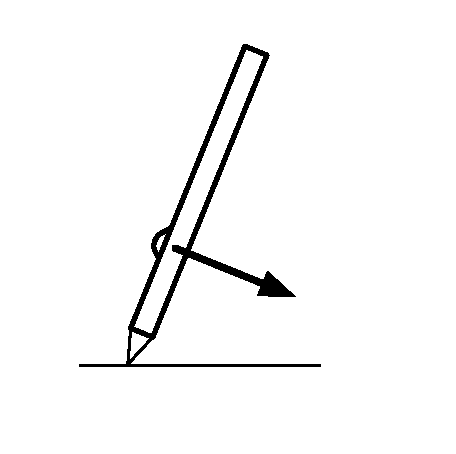
\includegraphics[origin=c, width=3.5cm]{img/button-force-pen.pdf}
}
\caption{The force required to press a mouse button compared with a
  stylus button.}
\label{fig:button-force}
\end{figure}

Some styluses have buttons. While buttons are an indispensable part of
a mouse, they are often difficult to use on the barrel of a
pen~\cite{plimmer-pen-usability}. The force of a \textit{mouse} button
click is orthogonal to the device's plane of use and has negligible
effect on target accuracy. However, pressing buttons on a
\textit{stylus} can move the tip of the pen, making it difficult to
press the button while pointing at particular objects (see
Figure~\ref{fig:button-force}). Further, pressing a button on a
computer stylus usually requires the user to adjust the pen in
hand. This action may be distracting and uncomfortable for long term
use.

\section{Large displays for drawing}

Groups of people often gather around traditional whiteboards to
brainstorm or exchange ideas. They draw pictures and diagrams,
maintain lists of text, and so on.  Whiteboards are also effective for
leaving asynchronous messages in the physical workspace where
co-workers can see them. People sometimes photograph whiteboards or
scan pages of sketches in order to record works-in-progress.

Electronic whiteboards such as the SmartBoard or those produced by
PolyVision more readily afford interactive usage than ordinary
whiteboards. For example, collaborative systems such as
Colab~\cite{stefik-colab} and Tivoli~\cite{pedersen-tivoli} support
meetings as people maintain checklists or collaboratively
draw. Systems can dynamically change their displays as people interact
with them, resizing or moving objects, or checking items in a
list~\cite{mynatt-flatland}. Large displays let more people have
simultaneous access to the drawing surface, which presents challenges
in sensing, and distinguishing between different users' pens.

Large displays have historically lacked portability, requiring a good
deal of time to install and calibrate. However, Lee recently
demonstrated a portable approach for projecting images on large
surfaces such as walls or tables, shown in
Figure~\ref{fig:lee-display}~\cite{lee-3d-infrared-pen}. The projector
emits patterns of time-multiplexed visible and infrared light. The
infrared light is decoded by sensors, providing a host computer with
fast and accurate location detection. The system uses sensors embedded
in the display surface to calculate the surface size and orientation
relative to the projector. Sensors may also be embedded in objects
such as pens, enabling alternate methods of user input. Equipping a
pen with a focusing lens allows it to become a short-distance pointing
device as in
Figure~\ref{fig:lee-display-2}~\cite[p. 62]{lee-projector-thesis}.

\begin{figure}
\centering
\subfigure[]
{
    \label{fig:lee-display-1}
    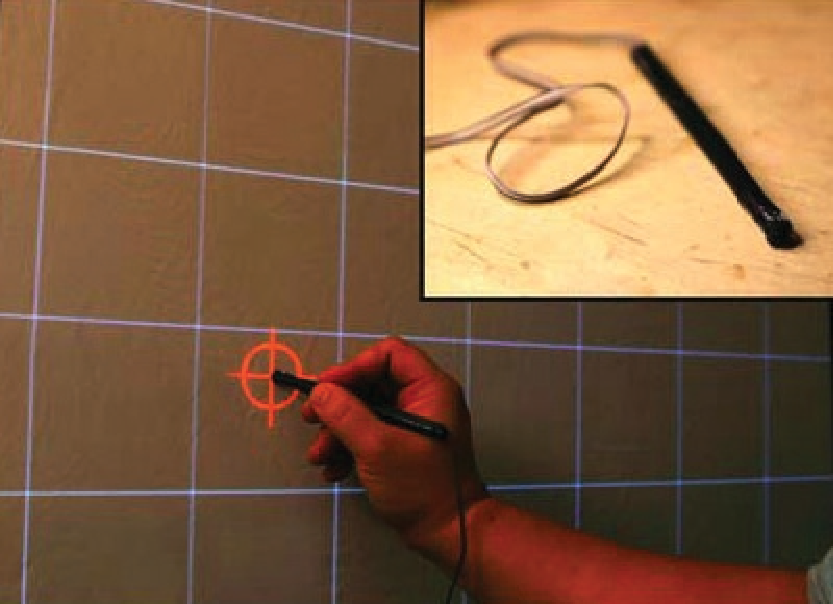
\includegraphics[origin=c, width=5cm]{img/lee-display-1.pdf}
}
\subfigure[]
{
    \label{fig:lee-display-2}
    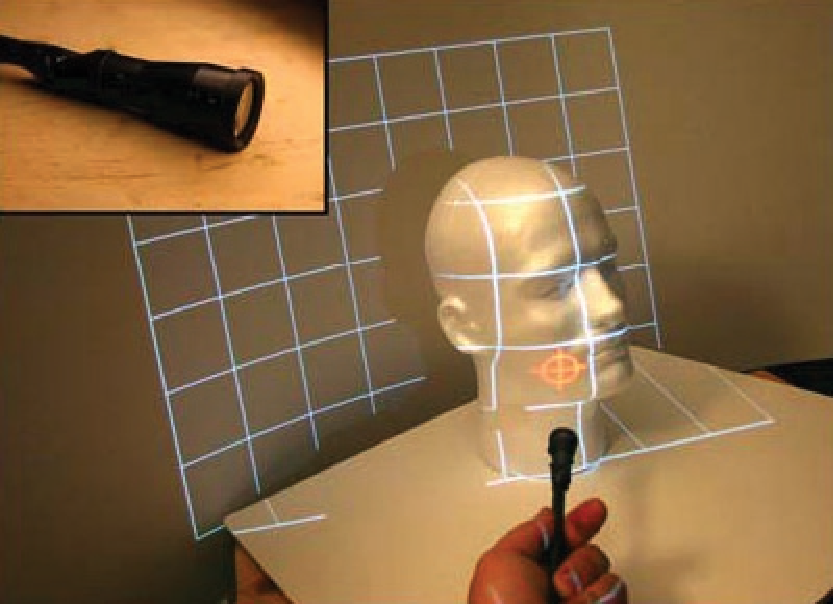
\includegraphics[origin=c, width=5cm]{img/lee-display-2.pdf}
}

\caption{Lee's portable projection approach enables detection of
  drawing surface size and orientation as well as pen input. This is
  effective on flat surfaces as in \subref{fig:lee-display-1} or
  curved surfaces as in \subref{fig:lee-display-2}.}

\label{fig:lee-display}
\end{figure}

At least two methods for capturing marks on ordinary whiteboards
utilize physical ink-like markers. The first uses traditional markers
whose activity can be detected by nearby sensors or cameras as the
user works, such as the Mimio commercial system. Whiteboard markers
are placed in sleeves whose position is calculated by the system
hardware.  Ju \textit{et. al} used a Mimio in the
WorkspaceNavigator~\cite{ju-navigator}.  PARC's
ZombieBoard~\cite{moran-collage-zombie,saund-zombie} used the second
method: scanning the whiteboard optically using a still camera. The
ZombieBoard enabled users to interact with the computer by drawing
special symbols. For example, users could delimit a region of the
whiteboard to be scanned by drawing its boundary. To invoke the scan,
the user would draw a button on the region boundary and draw an X or
check mark inside.



\newpage
\chapter{Sketch Recognition Techniques}
\label{sec:recognition}

Just as speech and gesture recognition gives us powerful new
interaction avenues, sketch recognition allows a different paradigm
for interacting with computers. This section summarizes strategies for
performing sketch recognition.

An important subset of sketch interpretation is handwriting and
character recognition, which is responsible for converting a person's
handwriting into text. Microsoft's Tablet PC API includes handwriting
recognizers for several languages, as well as symbol and gesture
recognizers for notation systems such as music or mathematics. The
recognition supported by the Tablet PC and other commercial
handwriting recognizers (e.g. Apple's Inkwell~\cite{apple-inkwell}) is
more closely aligned with what Larkin and Simon refer to as
``sentential''~\cite{larkin-diagrams}, as user input is expected to
proceed in a linear, serial fashion. This contrasts with
``diagrammatic'' representations that are expressed over a 2D plane.

Modern pen based computer systems like PDAs or Tablet PCs have
handwriting recognition software that has usable accuracy
rates. Recognition accuracy is typically measured by the deviation
between what the user intended and the machine's
interpretation. \textit{Error tolerance} refers to the recognition
inaccuracy rate a user is willing to accept. One study involving a
modified typewriter found that typists do not notice a word 0.5\%
error rate, 1\% is manageable, but 2\% is
unacceptable~\cite[p. 79]{cole-survey}. It is unclear if there are
similar accuracy thresholds for sketching, though studies have been
conducted for related recognition tasks. For handwriting recognition,
adults find 3\% minimally acceptable, with 1\% considered ``very
good''~\cite{lalomia-recognition-accuracy}. The acceptable accuracy
level depends a great deal on the expected benefit of the task. Users
will accept 20\% error rates if the tool brings greater productivity,
but are intolerant of errors\footnote{It is unclear if the values
described in these articles measure \textit{character} or \text{word}
recognition error rates. Santos \textit{et. al} describe handwriting
recognition error rates of approximately 10\% in terms
of \textit{characters}~\cite{santos-handwriting-recognition}.} when
the perceived benefit is
smaller~\cite{frankish-recognition-tolerance}. Another study examining
user acceptance of hand gesture recognition error rates found users
would tolerate mis-recognition up to 10\% when equivalent keyboard
commands could be employed~\cite{karam-gesture-recognition}.

There are a number of methods for improving recognition. Many PDAs
recognize characters from a constrained symbols set (Latin letters,
Arabic numerals), using different areas of the input surface for
drawing numbers and letters. This approach is not natural, but many
users quickly learn the alternate way of writing. In contrast,
Microsoft's Tablet PC handwriting recognizer allows people to write in
their own handwriting, at any location or angle. Microsoft's
recognizer incorporates a language model (e.g. spelling, grammar) to
guide interpretation.

Recognition is the centerpiece of many software prototypes that
support sketching. Although the research focus of many systems is not
recognition, such systems use automatic interpretation of sketches to
explore new methods of interacting with computers and new ways of
designing~\cite{gross-boe,grundy-maramasketch,lin-denim}. Such
projects rely on reasonably accurate recognizers. Recognition is
therefore a topic that affects nearly all aspects of research on
sketch based systems. For this reason, a substantial portion of this
review is devoted to aspects of sketch recognition. This includes
timing issues, determining what to recognize and how those elements
can be recognized, and interaction issues (see
Table \ref{tab:recognition-topics}).

\begin{landscape}
\begin{table}
\begin{tabular}{p{5cm}| p{2cm} | p{8.5cm}}
\textbf{Topic} & \textbf{Section} & \textbf{Remark} \\
\hline \hline
When to recognize & 
\ref{sec:recognition-when} &
Recognition is powerful but may also distract users from their
task. 
\\ \hline
What to recognize &
\ref{sec:recognition-what} & Sketches may represent objects
(e.g. tables and chairs) and spatial or functional relationships
between those objects (e.g. chairs positioned around table perimeter).
\\ \hline
How much to recognize &
\ref{sec:recognition-how-much} & 
Sometimes only a portion of a sketch need be recognized.
\\ \hline
How to segment &
\ref{sec:recognition-segmentation} &
Sketches contain many different symbols that may overlap. Recognizers
must isolate groups of marks for consideration.
\\ \hline
How to recognize &

\ref{sec:recognition-techniques}, \ref{sec:recognition-patterns}, 
\ref{sec:recognition-3d} &

Many recognition techniques exist, and are reliant on segmentation
methods. \\ \hline

Training recognizers &
\ref{sec:recognition-training} &
In order to recognize something we first need a concept of whatever is
to be recognized. \\ \hline

Managing recognition error &
\ref{sec:recognition-difficulties} &
Recognition sometimes results in inaccurate, ambiguous, or undesired
results.
\\ \hline
Reacting to recognition &
\ref{sec:recognition-action} &
Upon recognition the system must determine how to respond: provide
visual feedback, issue a search query, or take no outward action. \\ \hline

Toolkits for recognition &
\ref{sec:recognition-toolkits} &
Software packages facilitate easier engineering of new recognition
systems.\\ \hline

\end{tabular}
\caption{Topics in sketch recognition}
\label{tab:recognition-topics}
\end{table}
\end{landscape}

\section{When to invoke recognition}
\label{sec:recognition-when}

It is important that sketching systems \textit{aid} design exploration
and not simply \textit{computerize}
it~\cite{negroponte-soft-arc-mac}. For example, a sketch recognition
system might zealously identify parts of the user's drawing as it is
made, replacing the rough sketch with lines or curves. This removes
the opportunity for reflection and re-interpretation that is so
important to the early phases of
design~\cite{schon-reflective,goldschmidt-dialectics,terry-creative-ui}. Premature
recognition may interrupt the designer's flow of thought and interfere
with the task at hand. Instead we may want the computer to eavesdrop
silently, and provide help only when we need it.

A system can provide the user feedback of sketch recognition on
different occasions: (1)~immediately after receiving a single stroke
of input, (2)~as the user works, when feedback may be appropriate,
(3)~only upon request, or (4)~never. Many interfaces attempt immediate
recognition of gestures for invoking commands, such as with marking
menus~\cite{kurtenbach-marking-menus} or PDA device character
input~\cite{palm}. This is commonly called \textit{eager}
recognition~\cite{blostein-diagrams-review}. Other
systems~\cite{gross-ecn-uist,igarashi-suggestive,alvarado-sketchread-uist}
perform recognition in the background, deferring judgment until
adequate information is available. This is termed \textit{lazy}
recognition. Most modern research prototypes take this approach. Last,
some systems wait until the user explicitly requests
recognition~\cite{landay-silk}, or avoid recognition
entirely~\cite{forbus-nusketch-battlespace}. Combinations of these
approaches are common.

One method for identifying sketch input is to sidestep the recognition
process altogether and tell the system what you are about to draw by
choosing from a list or pressing a button. Forbus and colleagues take
this approach as they ``engineer around the need for recognition'' in
their \textit{nuSketch Battlespace} system (nSB) for managing courses
of action for military
commanders~\cite{forbus-nusketch-battlespace}. In order to position an
object such as an armored unit or a movement path, the nSB user
selects an item from a palette of glyphs and draws on the map. The
system interprets the user's ink differently depending on which type
of object is selected. For example when placing military units, the
ink's centroid is taken as the intended location; when defining a
region for those units to defend, the boundary is used.

\section{What should be recognized}
\label{sec:recognition-what}

User input in sketch based applications may be provided in two broad
categories. The first category, often referred to as \textit{digital
ink}, includes stroke timing information. Time data might be used by
sketching applications to determine how quickly the user was drawing,
or when strokes were made relative to one another. Many recognition
algorithms depend on the presence of time information. The second
category describes user input for which time data is unavailable. This
category of sketch input is used by applications that depend on
scanned or photographed
input. Section \ref{sec:recognition-techniques} describes the
differences between these two categories of sketch input from the
recognizer's perspective.

Different kinds of design drawings (``model ink'') in many domains
might be recognized: artistic sketches, study sketches, drawings,
diagrams, schematics, blueprints, and so on. In addition to model ink
comprising those drawing types, user input may be interpreted as a
command (``command ink''). The particular rules about what should be
recognized depends on the domain (architecture or circuit design),
kind of model (floor plan or timing diagram), and other
application-specific requirements. Sketches often contain hand-written
labels or annotations, which are common targets of pen based
recognition.

Diagrams usually have a domain-specific grammar describing how
vocabulary items relate~\cite{lakin-vmacs-89}. For example, boxes may
connect to other boxes via lines, those lines may have arrowheads to
indicate direction. Diagrams are good candidates for recognition
because the various elements and their relations can be described
formally. Table \ref{tab:what} summarizes various recognizable
classes.

\begin{landscape}
\begin{table}
\label{tab:what}
\begin{tabular}{ p{4cm} | p{4.5cm} | p{5.5cm} }
\textbf{``What'' to recognize} & 
\textbf{Examples} & 
\textbf{Remark} \\ 
\hline \hline

Genre &
Mathematical graph, architectural floor plan, web site layout, circuit design &

It may be sufficient to recognize a sketch is of a certain kind
without asking the user. The program could assume the sketch is
in a certain domain.\\ \hline

Characters (writing) & 
Alphanumerics, math symbols & 
Usually with other characters, in words and sentences. \\ \hline

Geometric shapes & 
Dots, lines, rectangles, blobs &
Geometric shapes are often drawn in relation to others. \\ \hline

Spatial features &
A is contained in, is above, is larger than B &
Spatial relations among elements may influence recognition. \\ \hline

Entities &
Domain-specific notation such as diodes, transistors &
Contextual clues can help disambiguate semantics of domain symbols. \\ \hline

Artistic nuance &
Shadows, textures, color &
Ink that modifies an existing element, perhaps suggesting 3D shape. \\ \hline

Commands &
Object selection, delete, copy, move, etc. &
Command ink specifies operations on the drawing. \\ \hline

Intention &
Drawing's function or behavior, e.g. \textit{circuit breaker} & 
Requires detailed domain knowledge and reasoning. \\ \hline

\end{tabular}
\caption{Kinds of elements to be recognized}
\end{table}
\end{landscape}

Artistic sketches and those drawings meant to authentically convey
three dimensional form comprise a different recognition
challenge. Nealen \textit{et. al} (who are concerned with modeling 3D
form) suggest that ``sketching a shape is inverse NPR
(Non-Photorealistic Rendering)''~\cite{nealen-3d-sketch}. Drawings
indicating physical form are not symbolic in the way diagrams are, and
not all drawings of 3D objects are necessarily meant to capture
literal shape. For example, many consumer products come with assembly
instructions featuring simplified diagrams of 3D objects to draw
attention to only those features and relationships relevant for
assembly.

Perhaps the most useful aspect of a sketch is the intention it
captures. The circuit breaker shown in
Figure~\ref{fig:circuit-breaker} probably would not work correctly if
it were manufactured exactly as shown, yet the intent of the drawing
is clear to a person familiar with such engineering
sketches~\cite{stahovich-sketchit-diagram}.

\begin{figure}
\begin{center}
  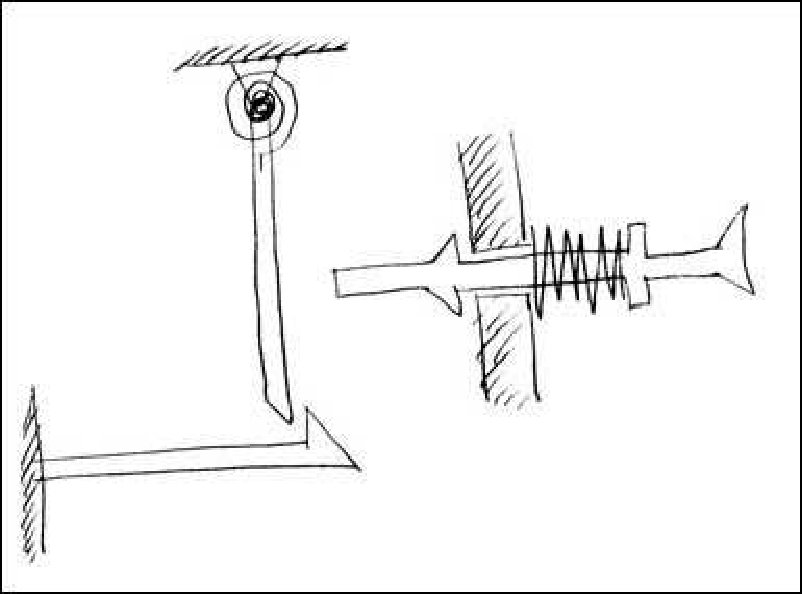
\includegraphics[angle=0, origin=c, width=2.6in]{img/circuit-breaker.pdf}
  \caption{A sketched circuit breaker~\cite{stahovich-sketchit-diagram}.}
  \label{fig:circuit-breaker}
\end{center}
\end{figure}

\section{How much recognition is appropriate}
\label{sec:recognition-how-much}

The nuSketch Battlespace system shows that a sketch based system need
not support recognition at all~\cite{forbus-nusketch-battlespace}. It
aims to enable users to quickly work with spatial data and issue
commands that operate on that data. To support this goal, nSB only
utilizes some properties of the user's ink. For example, the boundary
or center of the ink may be important, but the system need not
recognize the ink as a particular symbol.

Designers often create paper ``storyboards'' for showing high-level
structure or expected behavior without needing to specify
details. DENIM (for web site designers) and DEMAIS (for multimedia
designers) allow users to create such
storyboards~\cite{lin-denim,bailey-demais}. Both these systems
recognize a limited subset of the user's sketch input. Ink that is not
interpreted as belonging to a special set of gestures or symbols is
simply left on the canvas. This allows designers to capture ideas by
sketching naturally without being interrupted by unwanted feedback.

\section{Segmentation and grouping}
\label{sec:recognition-segmentation}

Segmentation and Grouping are related processes of breaking down user
input and finding related ink. Segmentation involves partitioning
undifferentiated sketch input into parts (analogous to identifying
word boundaries in speech recognition~\cite{cole-survey}). Grouping is
the process of forming logical collections of data (analogous to
determining which spoken words compose a sentence).

It is sometimes appropriate to break apart continuous pen strokes into
multiple segments, for example in recognizing cursive writing, or
finding corners in continuous pen strokes. Alternately, it may be
necessary to group related strokes in order to recognize compound
objects such as a triangle drawn with three distinct strokes. To
further complicate matters, there may be a number of reasonable ways
to segment user input~\cite{mankoff-burlap}, based on information such
as pen speed, stroke order, perceptual qualities, domain knowledge or
curvature~\cite{kim-segmentation}. Multi-modal systems may be able to
use additional information such as a user's speech or pointing
gestures to help segment and recognize
sketches~\cite{oviatt-multimodal,anthony-multimodal}. Which
segmentation technique is appropriate depends on what kind of sketch
input the application expects. The technical challenge is simplified
if the system requires users to complete each symbol before moving on
to another, or if each symbol must be drawn using a conventional
stroke order. However, such requirements work against the goal of
supporting unconstrained, fluid sketching.

The following describes three strategies for segmenting and grouping
continuous input strokes. They include the use of temporal data,
perceptual organization, and delimiter-based approaches.

\subsection{Temporal segmentation techniques}
\label{sec:recognition-temporal}

A common and effective method for segmenting ink is to use
time. Temporal data comes in (at least) three flavors. First, we may
look at the order strokes are made. For example, the letter $t$ is
usually drawn with the vertical stroke followed by the horizontal
crossing. Second, timing information for individual $(x,y)$ points tells
us how fast the user was drawing at any given location, which helps
identify corners. Last, a significant delay between individual strokes
may be interpreted as a delimiter between elements, just as a pause in
speech may indicate two distinct sentences.

Even for simple sketches there may be a very large number of possible
ways to segment ink. We can use stroke ordering to reduce
computational complexity of grouping and
recognition~\cite{sezgin-temporal}. Sezgin notes that common
depictions (like stick figures) tend to be drawn using one of a small
set of stroke orderings. However, it is also common for people to
begin drawing one recognizable entity \textit{X}, move to another, and
return to complete \textit{X} later on. For example many people cross
their \textit{t's} and dot their \textit{i's} after writing all
letters of a word. In Sezgin's terms, the user's marks
are \textit{interspersed}.

Another use of time for grouping ink looks at the velocity of the
stylus as the user moves it, to identify locations of interest such as
corners~\cite{sezgin-early-processing,davis-siggraph-tutorial}, or
places where the drawer may be taking extra care to be precise.

A series of strokes with short intervals may constitute a recognizable
entity. For example, people may draw a compound entity like a
television as a square enclosing a circle with a \textit{V}-shaped
antenna along the top. People tend to draw the three parts right after
one another, and then pause to think about what to do next. A
significant pause between pen activity might delimit objects. Such
timeout-based approaches are easy to implement but some users find it
imposes an unnatural feel to the
application~\cite{fonseca-fuzzy-recognition,zeleznik-sketch}.

\subsection{Perceptual organization}
\label{sec:recognition-perceptual-org}

Spatial data can also help with ink grouping. A simple location-based
approach forms groups based on ink proximity: if stroke \textit{A}
overlaps or comes close to overlapping stroke \textit{B}, group them
together. However, this strategy breaks down if distinct entities
overlap.

Gestalt psychologists offer the \textit{laws of perceptual
organization} to explain how people make sense of visual
scenes. Humans perceive scenes not only using what is shown but also
with ``invisible extensions as genuine parts of the
visible''~\cite{arnheim-visthink}. The rules of perceptual
organization include \textit{proximity},
\textit{similarity}, \textit{closure}, \textit{continuation} and 
\textit{common fate}~\cite{kanizsa-gestalt} (see Figure~\ref{fig:gestalt}). 

\begin{figure}
\centering
  \subfigure[] { 
    \label{fig:gestalt-proximity} 
    
\includegraphics[width=3cm]{img/gestalt-proximity.pdf} 
  }
  \hspace{2mm}
  \subfigure[] { 
    \label{fig:gestalt-similarity} 
    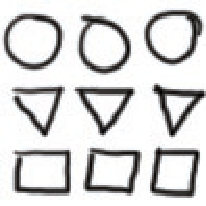
\includegraphics[width=3cm]{img/gestalt-similarity.pdf}
  }
  \hspace{2mm}
  \subfigure[] { 
    \label{fig:gestalt-symmetry} 
    
\includegraphics[width=3cm]{img/gestalt-symmetry.pdf}
  }
  \hspace{2mm}
  \subfigure[] { 
    \label{fig:gestalt-continuation} 
    
\includegraphics[width=3cm]{img/gestalt-continuation.pdf}
  }
  \hspace{2mm}
  \subfigure[] { 
    \label{fig:gestalt-closure} 
    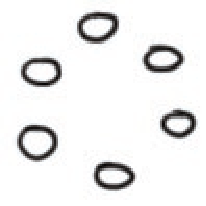
\includegraphics[width=3cm]{img/gestalt-closure.pdf}
  }

\caption{Some principles of perceptual organization~\cite{kanizsa-gestalt}. 
         \subref{fig:gestalt-proximity} Proximity: elements near one
         another are seen as belonging to a
         group. \subref{fig:gestalt-similarity} Similarity: objects
         sharing features such as shape belong in the same
         group. \subref{fig:gestalt-symmetry} Symmetry: two shapes
         symmetric about horizontal and vertical axes, suggesting they
         belong together. \subref{fig:gestalt-continuation}
         Continuation: the simplest explanation is two straight lines,
         not four lines meeting in the
         middle. \subref{fig:gestalt-closure} Closure: A large circle
         emerges from an arrangement of smaller circles.}
\label{fig:gestalt}
\end{figure}

Perceptual organization supports grouping at many levels. At a
low-level, we can use perceptual rules to analyze the relationship
among individual ink strokes to find plausible groupings for
recognition. Mahoney and Fromherz show how perceptual organization
rules can reduce the number of plausible stroke groupings into a
ranked list of groups, which helps improve recognizer
efficiency~\cite{mahoney-sketching-issues}. For example, an object may
be drawn on top of background elements, as illustrated by the stick
figure and horizon from Figure~\ref{fig:cloud}. Because the horizon
has strong continuity from the left to the right of the stick figure,
it is plausible the two halves should be grouped. The marks forming
the stick figure are in close proximity, and share similar sizes,
suggesting they may form a logical whole.

PerSketch and ScanScribe explore how perceptual organization rules can
be used on a number of
levels~\cite{saund-persketch,saund-perceptual}. Drawings are analyzed
in a manner approximating Marr's three-stage visual information
processing theory~\cite{marr-visual-infoprocessing}. In the early
phase, ink is broken into ``elemental curve fragments'' called Prime
objects (Primitive objects in ScanScribe). In the middle stage, Prime
objects are put into plausible groups using perceptual organization
rules. These groups are called Composite objects. Composite objects
may include Primes as well as other Composites. In the last stage,
domain rules are applied to combinations of Composite objects,
identifying which combinations of composite objects are reasonable
according to the subject matter (e.g. chemical modeling or electrical
engineering).

Gennari \textit{et. al} propose a segmentation approach based on
finding dense areas of ink and areas where the perceptual qualities of
the ink changes~\cite{gennari-parsing}. The Gennari system analyses
input as the user draws, calculating features such as ink
density. This approach is designed to work for node-and-edge diagrams
whose symbols do not overlap.

\subsection{Context-aware segmentation}

Particular aspects of the domain's graphical language may afford the
opportunity to use clever strategies for segmenting ink. This section
describes two methods for forming groups of marks by analyzing ink.

\begin{figure}
\begin{center}
  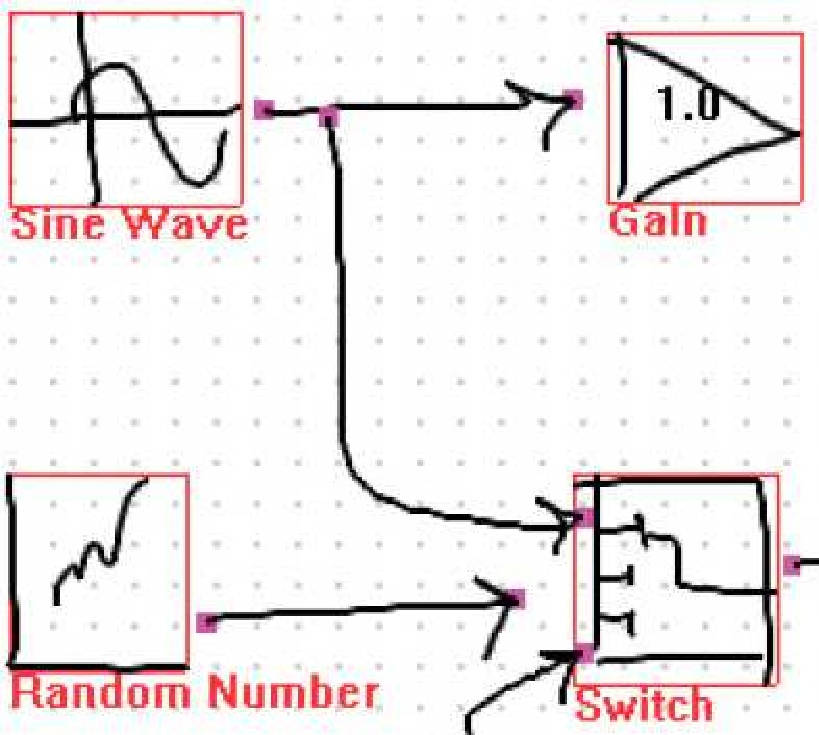
\includegraphics[angle=0, origin=c, width=2in]{img/simusketch.pdf}

  \caption{SimuSketch exemplifies delimiter-based, multi-phase parsing
  of sketches. The first stage identifies arrows as delimiters. In the
  second stage, clusters of remaining ink are recognized as domain
  symbols. }

  \label{fig:simusketch}
\end{center}
\end{figure}

Kara and Stahovich's SimuSketch is a sketch based interface for
creating graphical node-and-edge network diagrams in the Simulink
application. Simulink supports users in simulating dynamic systems
with a visual programming approach wherein boxes (nodes) represent
functions or processes, and connectors (edges) represent inputs and
outputs. SimuSketch looks for
\textit{markers} in the input sequence---easily identifiable 
symbols used to group other (non-marker) ink. In particular,
SimuSketch looks for edges between nodes (see
Figure~\ref{fig:simusketch}). 

Shilman's work on parsing handwritten notes incorporates context
awareness for discerning the structure of a sketched
document~\cite{shilman-discerning-structure} (see
Figure~\ref{fig:shilman-text-or-drawing}). Shilman's algorithm
integrates two related tasks in document analysis. The first challenge
is to discern marks as either writing or pictures. The second
challenge is handwriting layout analysis--grouping ink that has been
identified as writing into compound entities such as words, sentences,
and paragraphs. By combining these two processes,
Shilman \textit{et. al} can perform a limited feature-based
recognition on ink in order to test if it is text. The intuition is
that ``if you look at a page of ink with squinted eyes or from a
distance, you can distinguish writing from drawing by its regular,
linear structure.''  This approach uses features such as stroke length
and curvature as well as information derived from the spatial and
temporal relationship between fragments of ink. Marks are labeled as
either `text' or `drawing' using these local and global features with
a decision tree classifier.


\begin{figure}
\centering
\subfigure[]
{
    \label{fig:shilman-text-or-drawing-1}
    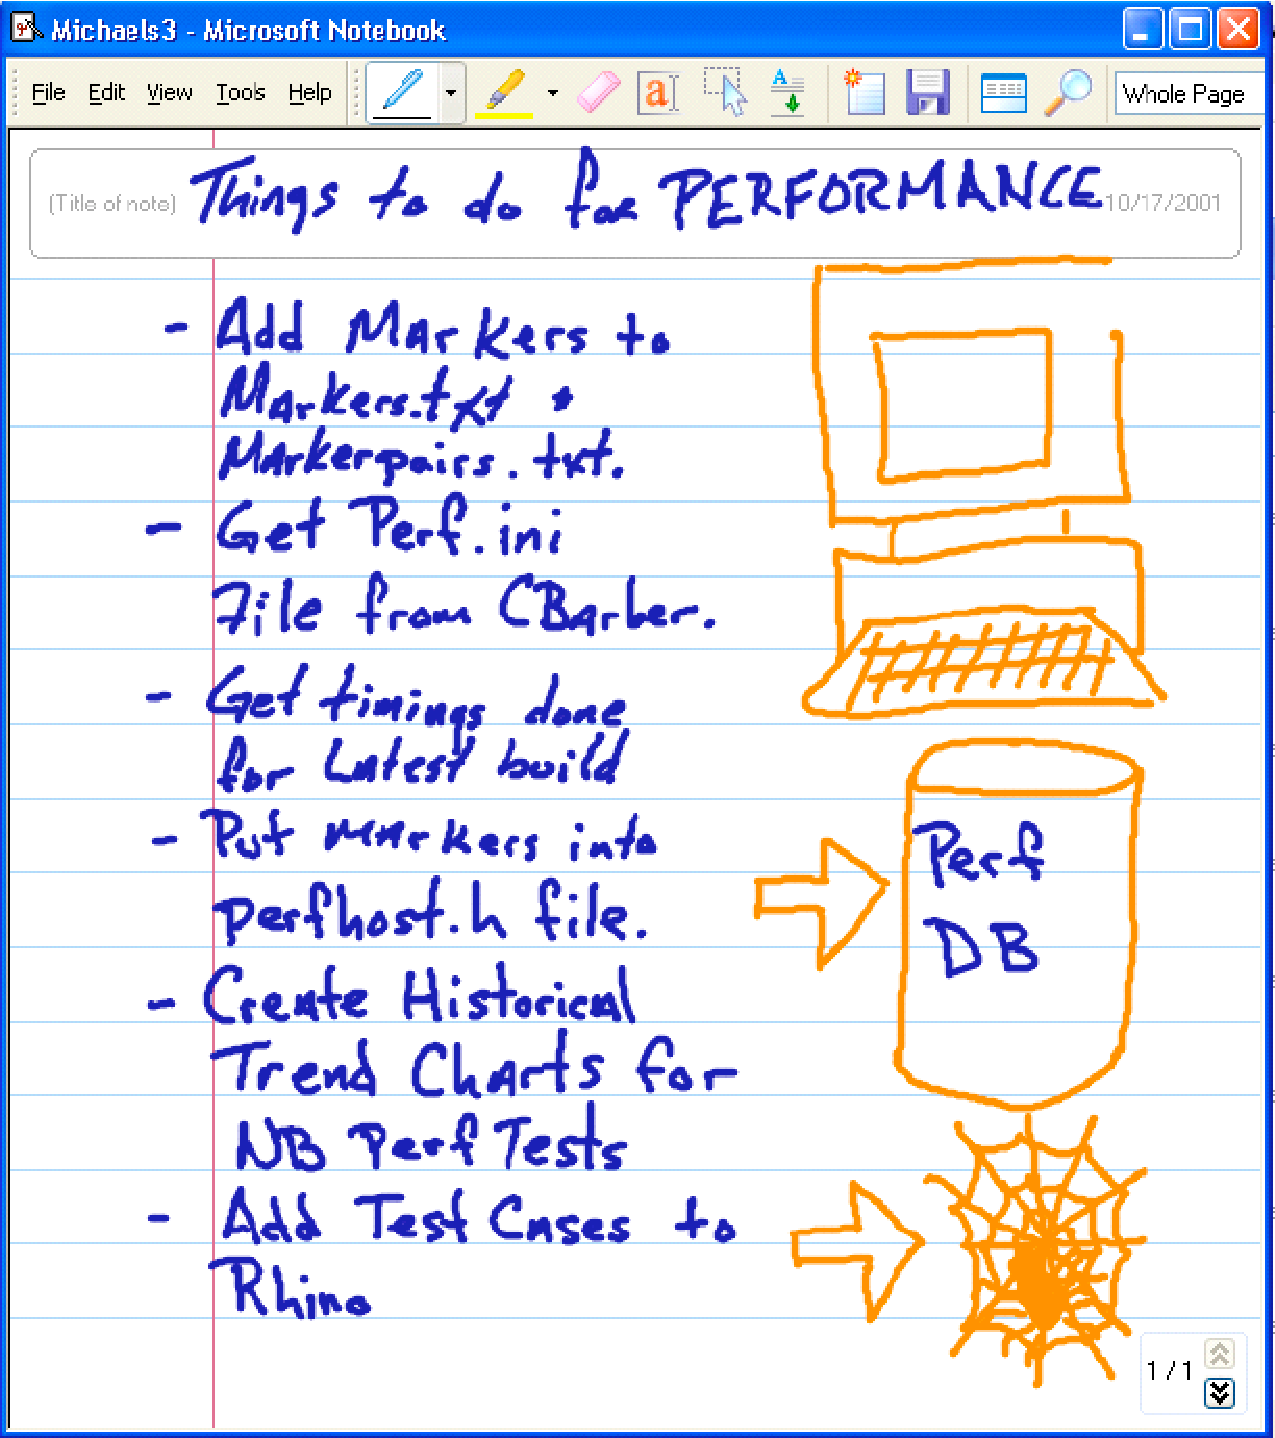
\includegraphics[origin=c, width=4cm]{img/shilman-1.pdf}
}
\hspace{1cm}
\subfigure[]
{
    \label{fig:shilman-text-or-drawing-2}
    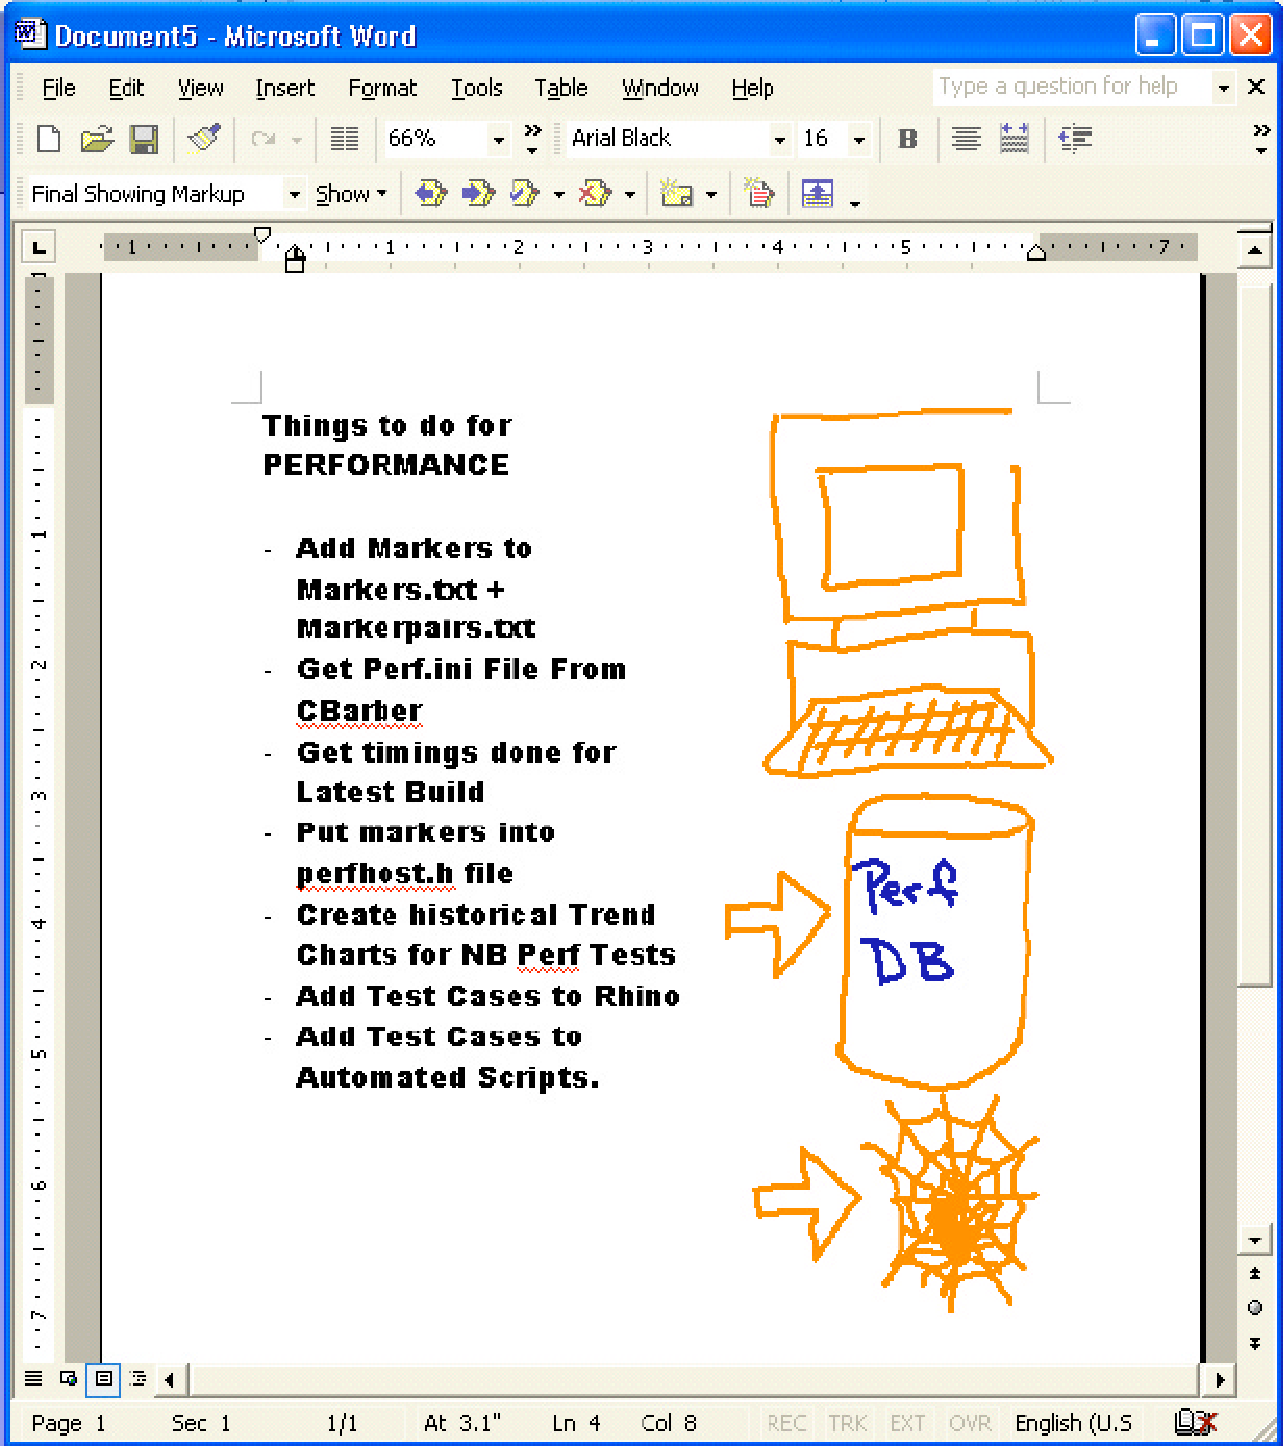
\includegraphics[origin=c, width=4cm]{img/shilman-2.pdf}
}

\caption{Analysis of hand-written notes discern writing
                  from drawings. Left: the original electronic
                  document. Right: the same document after handwriting
                  has been
                  recognized~\cite{shilman-discerning-structure}.}

\label{fig:shilman-text-or-drawing}
\end{figure}

\section{Overview of recognition techniques}
\label{sec:recognition-techniques}

This section gives a brief overview of various approaches for
performing sketch recognition.

Regardless of the input device, we identify two broad categories of
sketch recognition: \textit{on-line} and \textit{off-line}. On-line
recognition is analogous to your friend watching you sketch. Your
friend may see how fast you make a stroke, in which order you make
marks, and perceive what you say and how you gesture as you
sketch. Interpretation happens as the drawing is made. Off-line
recognition is analogous to your friend seeing your sketch for the first
time after you have finished it. Recognition happens after the drawing
is complete, irrespective of the order or speed strokes were
made. While off-line recognizers only have access to the finished
drawing, on-line recognizers potentially have access to data such as
pen pressure, time, speech, and gesturing.

Pen input is generally captured as a sequence of time-ordered 2D
coordinates. Other data such as pressure or (in a multi-user
environment) user identity may be available depending on the input
hardware. A single sequence of ink captured while the stylus is
touching the drawing surface is commonly called a \textit{stroke}.

On-line recognition strategies are further divided in two categories:
single-stroke and multi-stroke recognizers. Single-stroke recognizers
are appropriate for tasks such as interpreting freehand
gestures. Single-stroke approaches are simpler to implement than
multi-stroke strategies because user input is clearly divided into
pieces. This process could be relatively simple: a multi-stroke
recognizer might simply expect multi-stroke objects to be drawn in a
prescribed fashion. Or, multi-stroke recognizers might be more
complex, for example hypothesizing which individual strokes (or
segments of strokes) belong together, using Markov models or Bayesian
Networks to aid hypothesis testing.

We need some way of representing the \textit{entities} for
recognition. By ``entity'' we refer to classes that may be recognized:
boxes, lines, chairs, AND-gates, and so on (see also Table
\ref{tab:what}). The examples a recognition system has learned are
called \textit{classes}, and user's input are
\textit{candidates}. Three methods of presenting classes are covered
here: hard-coded, visual example, and textual description. Particular
instances of these methods are described later.

\subsection{Hard-coded recognizers}

One common approach is to hard-code recognition routines directly. For
simple or limited graphical vocabularies this may be appropriate. A
circle (or a zero, or the letter 'O', or the sun, etc.)  can be
recognized with a short program looking for input points that are
roughly equidistant from the stroke's centroid. However, ad-hoc,
hard-coded recognizers are difficult to maintain and extend. For
example, if we wished to extend our circle recognizer to interpret a
sun with rays of light coming out of it, we would have to also
recognize lines, then coordinate the recognizer to consider those
particular lines together with the circle, and ensure that the lines
are positioned and angled correctly. Further, sketch recognition
applications must be able to discern different kinds of elements. The
recognizers for each of these elements may conflict. A new recognizer
may cause an existing recognizer to stop working correctly, leading to
maintenance, debugging, and testing problems.

\subsection{Visual matching}
\label{recognition-library}

Another strategy for representing classes is to create a library of
drawn examples. Some techniques that use this approach are the Ledeen
recognizer~\cite{newman-sproull-graphics-2}, the Rubine
recognizer~\cite{rubine-recognizer}, Quill (based on
Rubine)~\cite{long-quill-chi}, Kara's
recognizer~\cite{kara-recognizer-cg}, and the \$1
Recognizer~\cite{wobbrock-dollar}. The accuracy of some of these
approaches can be improved if multiple training examples are
provided. Other techniques require only a single training example.

Some of these approaches are \textit{feature-based}. Such strategies
compute properties such as stroke length, stroke path, minimum or
maximum angle, or aspect ratio. A user's candidate entity is compared
with classes using these features. An alternate approach is to treat
visual examples as \textit{graphical templates}, where candidates and
classes are compared using some form of distance function.

User tests of recognition systems employing visual libraries commonly
include 30 or fewer classes~\cite[page 13]{kara-recognizer-cg}. For
many applications a database of that size is appropriate. It is
unclear how large these database can be: on one hand, human users have
limited ability to recall how uncommon symbols must be drawn; on the
other hand, recognition systems must search its (potentially
extensive) library for matches. The larger the database, the greater
probability of matching multiple classes, possibly leading to
ambiguity.

Library-based recognition schemes differ in how quickly the algorithm
searches its class database. Quill and the Rubine Recognizer compare
user input to each symbol, while other strategies (such as Kara's
recognizer) use efficient methods that exclude large portions of the
library before performing computationally intensive comparisons on the
remaining symbols. All of the methods discussed in the previous
paragraph provide interactive performance on the target hardware. For
example, the 1\$ recognizer produced results within about one second
using a consumer-grade PDA from 2006 with 16 symbols in the
recognition library~\cite{wobbrock-dollar}.

\subsection{Textual description}

Classes may be described textually using a programming
language~\cite{pasternak-adik,bimber-sketch-bnf,costagliola-xpg,hammond-ladder}. These
notations have two primary strengths. First, humans can read them. The
television symbol described in Section~\ref{sec:recognition-temporal}
may be described with natural language as ``a square with a slightly
smaller circle positioned at its center.'' A formal symbolic language
for that statement is still quite legible (assuming one understands
the function semantics):

\begin{verbatim}
      (define television 
              (and (centered square circle)
                   (slightly-smaller circle square)))
\end{verbatim}

Another strength of this kind of notation is that it allows the
developer to describe entities at a level of abstraction that
accommodates variability between entity
instances. An \textit{abstract} triangle is a three-sided,
two-dimensional convex shape whose internal angles sum up to
180\degree. A \textit{particular} triangle may have side lengths of 3,
4, and 5, and be oriented so that its long edge is horizontal. We may
define triangles and other entities as abstractly or concretely as the
language allows.

\subsection{Managing ambiguity}
\label{sec:recognition-managing-ambiguity}

Futrelle's classification scheme of types of ambiguity in diagrams
includes two high-level categories: lexical and structural
ambiguity~\cite{futrelle-ambigutiy}. Lexical ambiguity refers to the
``word'' level, when the meaning of a particular symbol is in
question. Structural ambiguity refers to confusion arising from the
composition of symbols.

Shilman augments this scheme with two additional types of ambiguity
that arise in sketch recognition: label and attribute
ambiguity~\cite{shilman-parsing}. Label ambiguity is present when the
symbol's identity is unclear. For example, a quickly drawn rectangle
might be interpreted as a circle. Attribute ambiguity refers to the
features of a sketched element: the exact location of a quickly drawn
rectangle's corner may be unclear.

Two sketching systems that focus on managing ambiguity at different
stages of user interaction are BURLAP and SketchREAD. A technique
built into BURLAP~\cite{mankoff-burlap} addresses domain independent
ambiguity management at the GUI toolkit level, while
SketchREAD~\cite{alvarado-sketchread-uist} offers a method for using
domain knowledge to disambiguate domain symbols.

BURLAP is a calligraphic application based on SILK~\cite{landay-silk}
that enables people to draw user interfaces. As the user draws, BURLAP
forms a list of plausible interpretations. At some point the system
may need to pick one interpretation.  Mankoff \textit{et. al} call
this process \textit{mediation}, performed by agents
called \textit{mediators}. Some mediators may engage the user by
displaying a pick-list of choices or visually indicating the
ambiguity. Other mediators automatically execute and do not involve
the user.

BURLAP exemplifies a framework for mediating ambiguity in
recognition-based interfaces called OOPS~\cite{mankoff-oops}. OOPS
consists of a library of error correction and ambiguity management
techniques that work with existing GUI toolkits at the input-event
level.

Alvarado and Davis's SketchREAD system demonstrates a technique for
modeling recognition ambiguity~\cite{alvarado-sketchread-uist}. The
SketchREAD application is a domain-independent sketching tool. It
accepts a textual description of classes to learn to recognize in a
particular domain~\cite{hammond-ladder} (see
Section~\ref{sec:recognition-training}). SketchREAD uses Bayesian
Networks to reason about the user's input based on domain
understanding~\cite{alvarado-dynamic-bayes}.

Bayesian Networks also allow us to encode relations of compound
objects that can further influence the belief in a hypothesis.
Alvarado and Davis give an example from a circuit design
application~\cite{alvarado-sketchread-uist}. A diode is depicted as a
triangle with a line tangent to one of the corners and parallel to the
opposing triangle edge (see Figure~\ref{fig:diode}). A person
typically draws a triangle first. The system calculates the
probability $P(triangle)$ that the marks depict a triangle. In circuit
diagrams, triangles are strongly correlated with diodes, so at this
point there is a \textit{partial hypothesis} that the person is
drawing a diode. Next, when the diode's line is drawn the system
calculates $P(line)$. Because a diode consists of a triangle and a
line, the Bayesian Network tests the hypothesis that the drawing is a
diode by calculating the joint probability of the triangle and line
interpretations. Even if one of the two parts (triangle or line) were
drawn sloppily, the higher-level hypothesis \textit{diode} can guide
us to a meaningful interpretation. If additional information is
present (such as connecting wires), additional belief values can be
used to support or reject the hypothesis that the drawing depicts a
diode.

A nice property of this recognition strategy is that it supports
efficient re-interpretation on an ongoing basis as the user continues
to work. The system endeavors to make sense of each new input stroke,
making use of established interpretations and associated
probabilities. While na\"ive systems may exhaustively test all
possible interpretation hypotheses, SketchREAD's hypothesis pruning
enables the system to test only the most likely
interpretations. SketchREAD's interpretation speed scales roughly
linearly with the number of strokes, compared to the exponential
runtime used by some other approaches.

\begin{figure}
\begin{center}
  
\includegraphics[angle=0, origin=c, width=0.7in]{img/diode.pdf}
  \caption{A diode is drawn as a triangle with an adjacent line.}
  \label{fig:diode}
\end{center}
\end{figure}

\section{Pattern recognizers}
\label{sec:recognition-patterns}

Various methods have been investigated for performing recognition of
sketch input. The methods covered have been known variously as
character recognizers, glyph recognizers, and pattern
recognizers. They operate on isolated strokes or segments of strokes
and do not perform higher-level reasoning based on domain semantics or
context.

All these recognition approaches work using the same general strategy,
and although each has its own strengths and weaknesses, no single one
is best for everything. The general strategy has not changed since the
earliest on-line character recognition
systems~\cite{groner-grail-recognizer,newman-sproull-graphics-2}. The
first step is to learn a dictionary of \textit{classes}. These serve
as instances of the elements the recognizer can handle. The
recognition system converts user input into \textit{candidates}. The
candidate is then compared to classes in the dictionary, producing a
similarity metric for each comparison. Sketch based applications can
use higher-level methods to reason about the most likely choice or
choices. Alternately, the best match from the low-level recognizer
might be used.

While the recognition strategies described below share a high-level
strategy, they differ in how they represent candidates and classes and
how they are compared.

\subsection{Ledeen recognizer}

The Ledeen character recognizer is efficient and easily
trained~\cite{newman-sproull-graphics-2}. User input is scaled to fit
inside a three-by-three grid of nine cells. Each stroke's starting
cell is noted, and each stroke's path through the grid is
encoded. This approach accommodates multiple stroke input but does not
specify how multiple strokes should be grouped to be considered
together. Newman and Sproull suggest considering multiple strokes
together if less than half a second of latency separates strokes.

Some user input is not easily handled with this scheme. For example,
straight vertical or horizontal lines would require scaling one
dimension significantly more than another, leading to an unreliable
path order. Dots also give this approach trouble. Problematic strokes
like dots and vertical or horizontal lines are recognized by
special-case algorithms instead of the 3$\times$3 grid approach. GRAIL
employed a multi-stroke, context-sensitive recognition strategy very
similar to the Ledeen recognizer~\cite{groner-grail-recognizer}.

\subsection{Rubine Recognizer}
\label{sec:recognition-rubine}

Rubine's feature-based recognition approach was demonstrated by a
system called GRANDMA (Gesture Recognizers Automated in a Novel Direct
Manipulation Architecture). The features involve geometric properties
of single strokes such as start/end locations, total gesture length,
sine/cosine of initial angle, and so on. Each feature must be
calculable in constant time to ensure efficiency.

Some features are more effective than others for classifying a given
symbol. If a number of examples are provided (typically 15 or more
produce good results), the trainer uses linear discriminant analysis
to determine the most effective features for classifying a particular
entity.

Rubine's work was extended with a recognition system called gdt (later
renamed Quill)~\cite{long-quill-chi}, and added several feature types
such as aspect ratio and curviness. Quill was incorporated into
SATIN~\cite{hong-satin}, a toolkit for building sketch based
applications.

\subsection{Kara's Recognizer}

A recognition technique developed by Kara and
Stahovich~\cite{kara-recognizer-cg} differs from stroke-oriented,
feature-based approaches such as Rubine's. Instead, it compares the
spatial distance between down-sampled bitmap representations of
symbols. Kara's recognizer does \textit{not} rely on geometric
features like corners, angles or lines, and operates on input
regardless of temporal information. Further, it accommodates
multi-stroke entities as easily as single-stroke entities.

The technique first applies a polar coordinate transformation about a
cleverly chosen pivot point. Input is incrementally rotated from
-$\pi$ to +$\pi$ radians and compared with a class entity to determine
a rotation that best aligns two symbols. This ``pre-recognition'' step
helps exclude unlikely matches.

After rotating the user's input the algorithm creates an
\textit{n}$\times$\textit{n} down-sampled bitmap (\textit{n}=48 works
well). Next the recognizer applies four spatial distance classifiers
to compare user input against known classes. The results of each
classifier are converted into comparable forms and combined to produce
a single recognition value describing the similarity between the user
input and classes.

\subsection{Cali Recognizer}

Fonseca \textit{et. al's} non-trainable Cali recognizer can identify
geometric shapes at any angular orientation or aspect
ratio~\cite{fonseca-caligraphic,fonseca-fuzzy-recognition}. These
shapes may consist of any number of strokes, as they are segmented
based on a timeout (see Section~\ref{sec:recognition-temporal}). To
identify the shape (triangle, cross, etc.) Cali first finds geometric
properties based on the input: the convex hull, the largest triangle
and quadrilateral inscribed inside the hull.  Additional geometric
properties are calculated based on these shapes, including areas and
perimeter values and aspect ratios. These values are then used to
search through prior statistical data regarding the shapes to be
recognized. This approach uses fuzzy logic to determine membership in
statistical equivalence classes. For example the recognizer for the
shape ``Line'' reports true if the input's aspect ratio ``is very
thin''.

A trainable variant of Cali compared several learning algorithms for
building the statistical equivalence classes: K-nearest neighbors,
inductive decision trees, and Naive Bayesian Networks. Testing showed
Naive Bayesian Networks the easiest to train with the best recognition
rates.

\subsection{\$1 Recognizer}

The \textit{\$1 Recognizer}~\cite{wobbrock-dollar} is notable because
of its ease of use, algorithmic elegance and power. This technique is
designed for use on PDA-like devices that accept pen based, gestural
input for characters and commands. The \$1 Recognizer requires only a
single training example to be effective. Users may easily create their
own gestures---it is trainable on the fly.

The algorithm processes candidate and class input the same way. It
begins by resampling input into a number of points (n=64 was found
adequate). This enables \$1 to compare strokes of different sizes and
drawing speeds. Next, the input is rotated so the angle formed by the
input's centroid and initial point is 0\degree. After rotation the
input is scaled non-uniformly to fit inside a square. Like the Ledeen
algorithm, the \$1 Recognizer must handle certain classes of input
(e.g., straight lines) differently because scaling the input
non-uniformly would distort it too much. Last, the candidate is
compared to each class in the dictionary by summing the error of
corresponding points.

\subsection{Graph matching techniques}
\label{sec:recognition-graph}

\begin{figure}
\begin{center}
\subfigure[] {
  \label{fig:llados-graph-1}
  
\includegraphics[origin=c,height=1.0in]{img/llados-1.pdf}
}
\subfigure[] { 
  \label{fig:llados-graph-2}
  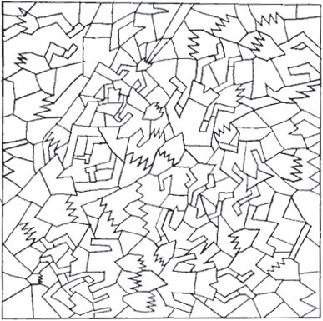
\includegraphics[origin=c,height=1.7in]{img/llados-2.pdf}
}
\subfigure[] { 
  \label{fig:llados-graph-3}
  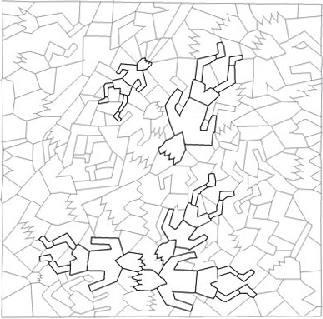
\includegraphics[origin=c,height=1.7in]{img/llados-3.pdf}
}
\caption{Example of graph-based pattern matching~\cite{llados-rag}. An
  example pattern is shown in \subref{fig:llados-graph-1}. The complex
  test image in \subref{fig:llados-graph-2} contains several
  distorted, scaled and rotated instances of the pattern. Portions of
  the example pattern found in the test image within acceptable error
  tolerance are shown in \subref{fig:llados-graph-3} with thick
  lines.}
\label{fig:llados-graph}
\end{center}
\end{figure}

The techniques discussed earlier are best used for on-line recognition
because they require timing data regarding stroke path (e.g. Ledeen's
approach) or where strokes begin and end (e.g. \$1 or Kara
recognizers). But on-line recognition is not always possible. A
designer may scan a paper sketch and expect to use it as the basis for
further work. In such cases, off-line recognition might be
employed. Graph-based recognition techniques are commonly used for
this purpose in the document analysis and engineering diagram research
community.

The first step in graph-based off-line recognition is to convert the
input image from a raster to a vector
representation~\cite{tombre-vectorization}. Vector endpoints and
junctions form graph nodes, and edges represent lines between
them. Because graph nodes contain additional information such as
$(x,y)$ position, these structures are called \textit{attributed
relational graphs}.

A full drawing's corresponding graph can be searched for identifiable
portions, or subgraphs using \textit{subgraph isomorphism}
algorithms~\cite{lee-graph-matching}. Llad\'{o}s has proposed an
heuristic technique for error-tolerant pattern matching using subgraph
isomorphism~\cite{llados-rag}. For example, suppose we are interested
in finding the pattern shown in Figure~\ref{fig:llados-graph-1} in the
test image shown in Figure~\ref{fig:llados-graph-2}. After converting
both the example pattern and the test image to attributed relational
graphs, this technique begins searching through the test image graph
for sequences that resemble the example pattern's graph. When this
algorithm finds a near match, it employs edit operations on the test
image graph to force an exact match. Recognition confidence is
measured in terms of how much the observed graph must be edited in
order to match the expected graph. As shown in
Figure~\ref{fig:llados-graph-3}, the approach is rotation and scale
invariant and tolerates some degree of distortion.

\section{Recognition of 3D scenes}
\label{sec:recognition-3d}

Although many sketches represent abstract entities that lack physical
form (e.g. UML diagrams), many others have physical, three-dimensional
interpretations. In this section, ``recognition'' refers to
reconstructing 2D sketch input as 3D models. In this sense the
recognition is syntactic (e.g. identifying a rectangular
parallelepiped) rather than semantic (e.g. identifying a shoe
box). Reconstruction of 3D scenes has been studied in the robotics and
computer vision community as well as by CAD researchers.

3D recognition is essentially ``reverse projection''. The strokes on
the drawing surface provide $(x,y)$ data but not depth
$(z)$~\cite{lipson-correlation}. Because $z$ could take on any value
there are an infinite number of ways the 2D drawing could be turned
into a 3D model. Fortunately knowledge of solid geometry restricts the
possible interpretations: the surface of a 3D object can not pass
through itself, so any interpretation that involves self-intersecting
surface planes is invalid. There are many ways to compute particular
$z$ values for sketched 3D models. Analytic approaches include line
and junction coding~\cite{clowes-seeing-things,huffman-nonsense} and
solving linear equations~\cite{grimstead-3d-linear-system}. Other
approaches attempt to fit sketch input to likely constructions such as
primitive 3D structures such as cylinders~\cite{wang-3d-sketch}, or by
finding likely geometric constraints like parallelism and
symmetry~\cite{shpitalni-curve-fitting}. Many 3D sketch recognition
systems employ a combination of these approaches.

People can recognize sketches as long as they are made from a familiar
vocabulary. We also make inferences about 3D shape based on 2D
perceptual qualities such as parallelism, right angles, and alignment
to primary axes. Further, drawings of 3D objects often use shading to
show shadows and contours. Frequently when people draw a 3D object,
they draw only the visible contours, leaving the rest to the
imagination. It is not difficult to look at a box and be able to
``see'' the edges and corners that are obscured by the solid geometry
(although the imagined edges might in fact be wrong). Some have
developed heuristic methods for hidden-line
inference~\cite{mumford-hidden-line,karpenko-smoothsketch} that
``reconstruct'' a 3D object without access to a complete 2D
wireframe. A wireframe model shows edges in a ``see-through'' view;
hidden lines are shown through surfaces.

\begin{figure}
\begin{center}
  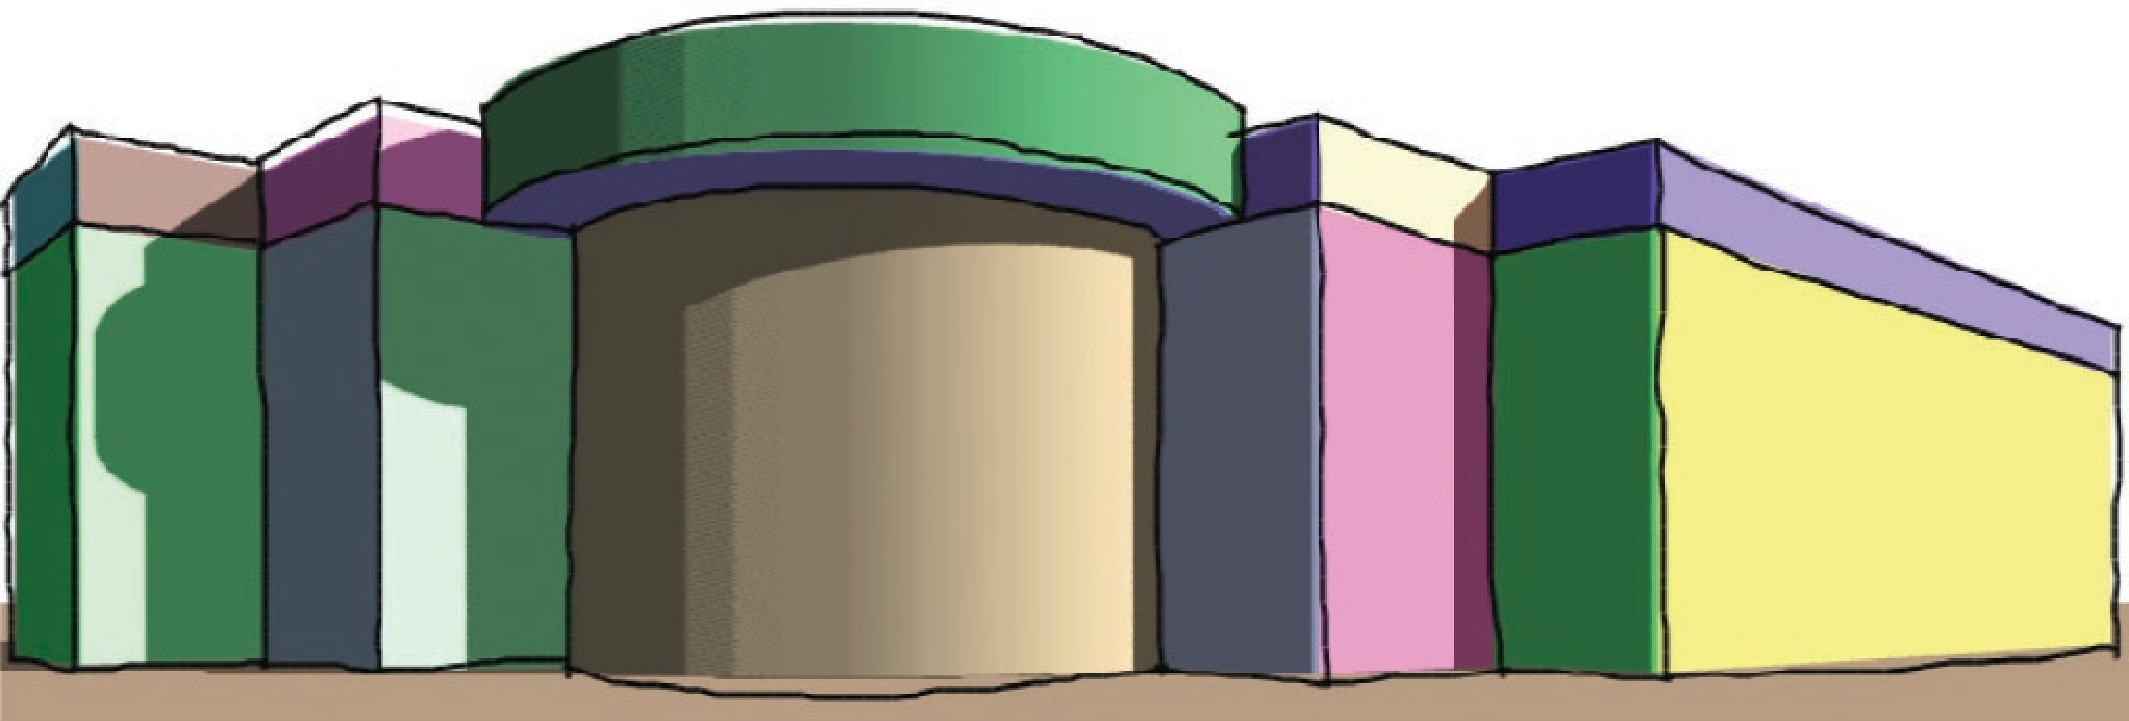
\includegraphics[width=3in]{img/sketching-reality.pdf} \caption{``Sketching
  reality'' allows users to create 2.5D architectural models by
  sketching~\cite{chen-sketching-reality}.}  \label{fig:sketching-reality}
\end{center}
\end{figure}

Design software need not reconstruct full 3D models to be
useful. Instead, the recognition system could build a 2.5D
interpretation of a 2D sketch. A 2.5D model contains depth information
only for geometry visible from a single vantage point, so the
recognition system is relieved of the difficult task of inferring the
full 3D structure. Recent work from Microsoft Research Asia
demonstrates an interactive 2.5D recognition and rendering
system~\cite{chen-sketching-reality}. Figure~\ref{fig:sketching-reality}
shows sample output of this approach.

\subsection{3D Curve Analysis}

\begin{figure}
\begin{center}
   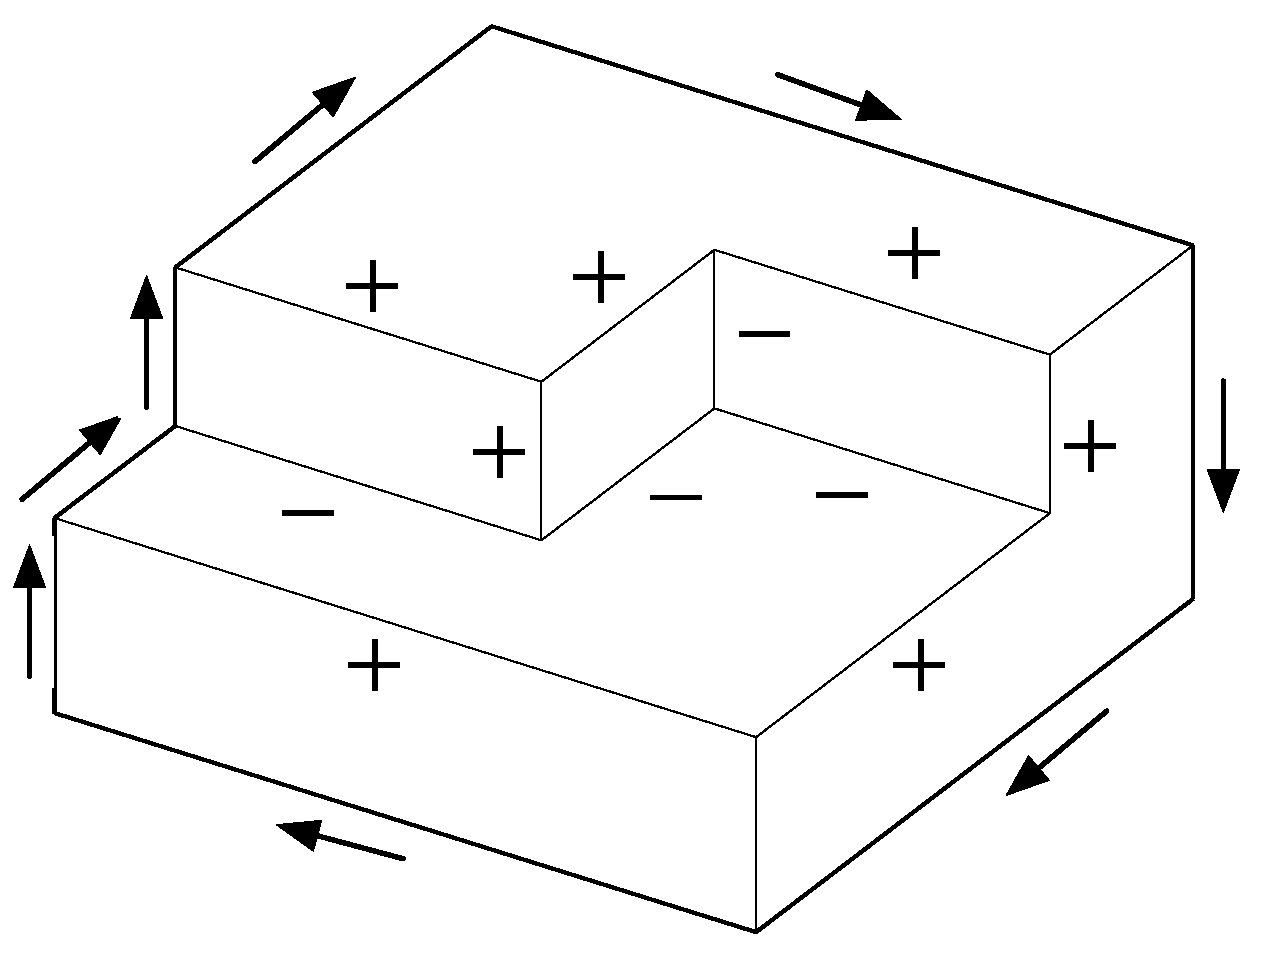
\includegraphics[origin=c,width=2in]{img/huffman-clowes.pdf} \caption{An
   illustration of Huffman-Clowes labels. Arrows indicate edges whose
   faces are obscured.  $+$ and $-$ identify edges as convex and
   concave.}  
   \label{fig:huffman-clowes} }
\end{center}
\end{figure}

3D recognition begins much the same way as 2D recognition. Individual
marks constituting a drawing are classified into features such as
lines, curves, and junctions. The recognizer must determine the
relationship between these features. For example, if a line represents
an edge between two faces, what is the dihedral angle?  There are a
number of ways to perform this analysis. Two are discussed briefly
below.

One approach to 3D stroke analysis is to label drawn and emergent
elements such as lines, vertices, and faces. The Huffman-Clowes
method~\cite{clowes-seeing-things,huffman-nonsense} identifies various
ways faces of a drawn polyhedron may relate (see
Figure~\ref{fig:huffman-clowes}). This helps reconstruct the 3D
geometry of the object based on the 2D drawing. A Huffman-Clowes label
indicates whether the line represents a concave or convex edge. Edges
are labeled ``obscuring'' if one of the adjoining faces is not
visible. Given a line drawing, there may be more than one possible way
to assign Huffman-Clowes labels~\cite{thorpe_huffman_clowes} (see
Figure~\ref{fig:necker}). Schweikardt and Gross used Huffman-Clowes to
interpret sketches of 3D objects in their Digital Clay
system~\cite{schweikardt-digital-clay}.

Shpitalni and Lipson use regression to classify input strokes and
clustering to identify 3D vertices shared by multiple lines. Stroke
classification fits input to conic sections using a linear system of
equations~\cite{shpitalni-curve-fitting}.  This approach is effective
for detecting straight lines, parabolic arcs, and hyperbolae. A sharp
(or filleted) corner, for example, can be found with a hyperbolic
conic section. After detecting curves, neighboring curve endpoints are
merged when appropriate.

\begin{figure}
\begin{center}
\subfigure[] { 
  \label{fig:necker-wireframe}
  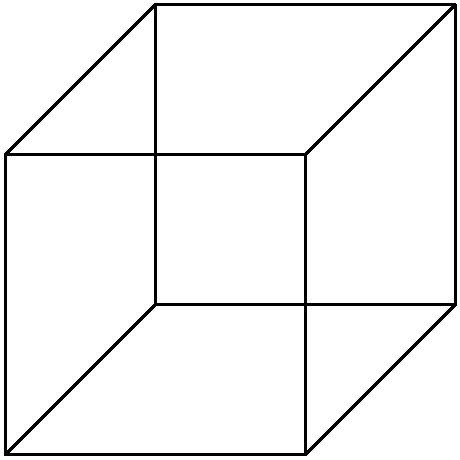
\includegraphics[origin=c,width=0.8in]{img/necker-wireframe-only.pdf}
}
\subfigure[] { 
  \label{fig:necker-interp-a}
  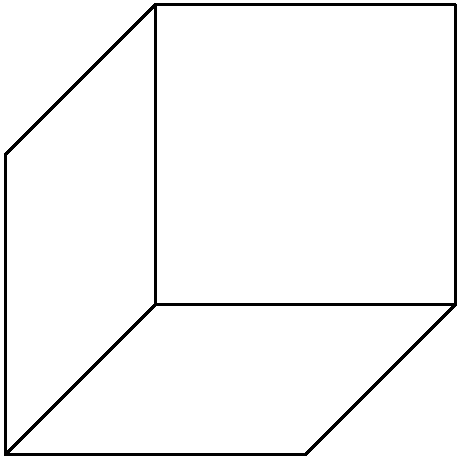
\includegraphics[origin=c,width=0.8in]{img/necker-interp-a.pdf}
}
\subfigure[] { 
  \label{fig:necker-interp-b}
  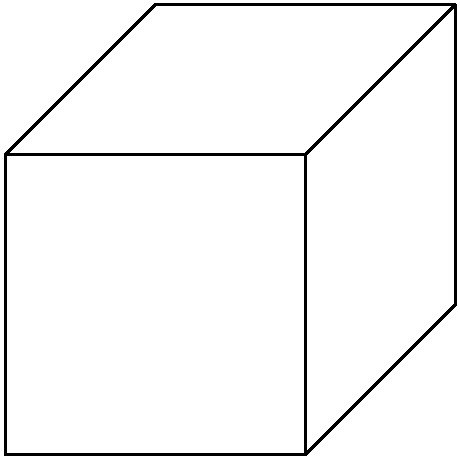
\includegraphics[origin=c,width=0.8in]{img/necker-interp-b.pdf}
}
\caption{A Necker Cube illustrates difficulty when forming 3D 
         interpretations of 2D line drawings. The wireframe shown
         in \subref{fig:necker-wireframe} can be interpreted in two
         equally valid ways, shown in \subref{fig:necker-interp-a}
         and \subref{fig:necker-interp-b} with hidden edges removed.}.
\label{fig:necker}
\end{center}
\end{figure}

\subsection{Gesture-based 3D recognition}

One way to provide input for a 3D sketching system is gestural
commands for creating or editing solid geometry models.
SKETCH~\cite{zeleznik-sketch} and
SKETCH-N-MAKE~\cite{bloomenthal-sketch-n-make} recognize gestural
commands to represent certain 3D forms. For example, when the user
draws two parallel lines, the system generates a cylinder. The drawing
direction defines whether the solid is additive (upward gestures) or
subtractive (downward gestures).

\subsection{Direct and indirect solid model drawing}

Teddy~\cite{igarashi-teddy} interprets user input as the outline of an
object. The object is then inflated to provide a smooth, blobby
object. Subsequent edits are done by explicitly changing modes and
entering commands as appropriate. For example, an object in Teddy may
be extended by drawing an attachment point on the existing object
followed by an outline of the new part of the object.

Not all the user's marks denote object boundaries. Designers draw
shadows, stipple dots, or little lines to indicate curvature or
surface texture. Cohen leverages this to create 3D models from
sketches by drawing shadows of objects~\cite{cohen-3d}. In this
system, ink is interpreted either as solid model geometry or as
the \textit{shadow} of that geometry projected onto a floor plane
below.

\subsection{Imposing and Inferring 3D Axes}

Finding depth values for vertices in a 3D sketch is easier if the
drawing conforms to an axis system, and if the object's faces are
known to be generally parallel to these axes. It may be reasonable to
impose a 3D axis scheme on the user. Alternately, the system can
interpret a user's drawing and infer an axis system.

Chateau allows people to design 3D objects (like French villa-style
buildings) using a constrained vocabulary of lines and
angles~\cite{igarashi-suggestive}. In Chateau, ink is interpreted as
wireframe elements that may connect to existing pieces on an explicit
``drawing plane''.

A coordinate system helps orient the user's marks so the overall
geometry can be found. However, some 3D sketching systems do not
provide a default 3D axis. The user may draw objects from any
perspective. One approach forms an Angular Distribution Graph (ADG)
showing how often lines are drawn at each
angle~\cite{lipson-correlation,masry-3d-sketch}. The ADG allows the
software to infer a coordinate system based on an analysis of the
drawing itself.

Tsang presents two methods for guiding 3D
reconstruction~\cite{tsang-3d-sketching}. In their system, recognition
works in the context of two kinds of guides. First, a 2D image may be
imported and placed in the drawing environment. The position and
curvature of sketched input is influenced by these images. Second, the
system analyses the drawing and suggests 3D wireframe models from a
database composed of prior work by the user or by third parties.

\subsection{Styling based on existing 3D geometry}

In many three-dimensional sketching systems, the visual representation
is often beautified during reconstruction from 2D to
3D. Beautification may substantially change the character of the
drawing so it no longer looks ``sketchy''. 

The work by Nealen and colleagues builds on the Teddy-like approach of
generating smooth 3D objects based on a
sketch~\cite{nealen-3d-sketch,nealen-fibermesh}. Users may draw on the
surface of 3D objects as a way to issue modeling commands. To stretch
a region of interest, the user first draws on the object to create the
control points, then drags them to stretch the surface.

Often designers create new instances of known object types. For
example, when designing the shape of computer speakers, designers work
from experience with other speakers. By providing a 3D wireframe that
is approximately the same shape as the desired object, a designer can
sketch around the wireframe to create a new
shape~\cite{mitani-3d-sketch,kara-3d-styling}. The user's marks are
recognized in the context of the wireframe, enabling the designer to
quickly create a new styled instance of an existing class of objects
without having to first make the wireframe.

A related approach is shown in the domain of organic plant
modeling~\cite{anastacio-plant-sketching}. Instead of a geometric
wireframe, this approach applies a mathematical model specifying the
target domain based on knowledge of plant biology. This technique
allows designers to quickly converge on a specific, highly refined 3D
model by sketching. To be sure, this advantage comes at the cost of
generality.

\section{Recognition training and domain modeling}
\label{sec:recognition-training}

In order for a sketch recognizer to interpret user input it first
needs a representation of whatever elements it is intended to
identify. There are two broad categories of methods for acquiring the
model from users. The first is to provide drawn examples; the second
is to provide written descriptions.

Many of the pattern recognizers discussed here provide user interfaces
for capturing training examples. In general these all work the same
way: users provide pen input and then label that input. The Rubine
recognizer and Quill require multiple training examples to determine
which analyzed features should be used to classify candidate input.

An alternative approach to providing drawn examples is to describe
symbols with some sort of text
description~\cite{mas-graph-grammar}. Costagliola \textit{et. al}
refer to these as \textit{Sketch Grammars}, or SkGs for
short~\cite{costagliola-skg}. A SkG is a BNF-like description of how
low-level elements like lines and circles can combine to form
higher-level elements. The combinations are described in terms of
geometric shapes and constraints describing their relative lengths,
positions, and angles. Once an entity's grammar is defined it may be
used to compose more complex elements. The grammar-based recognition
approaches covered here all share similar constraint types such
as \textit{parallel}, \textit{perpendicular}, \textit{above},
\textit{below}, \textit{smaller-than}, and \textit{centered-inside}.

Current work on sketch parsing leverages prior work from the visual
languages community. Lakin describes visual language parsing as ``the
process of recovering the underlying syntactic structure of a visual
communication object from its spatial arrangement.'' Lakin's vmacs
system~\cite{lakin-vmacs-89} supports users in providing unstructured
graphic input that can optionally be parsed by a visual grammar in
order to formally describe the structure of the depiction.

Grammar-based diagram parsing by Futrelle and Nikolakis focused on
parsing scientific figures as they appear in
publications~\cite{futrelle-diagram-parsing}. This research used
vector graphics rather than rough sketches, but it could be applied to
interpreting hand-drawn diagrams.

Compound objects were defined in the Electronic Cocktail Napkin (ECN)
as a set of elements and spatial relations~\cite{gross-boe}. The ECN
generated symbolic constraint descriptions from the user's sketch
input. The user could then modify the description by adding or
deleting constraints, or generalizing or making them more
specific. The ECN used a hybrid recognition approach involving a
low-level pattern-based recognizer to identify symbols and a
high-level grammar-based approach to recognize pattern configurations.

Constraints are often used to prescribe relations between elements
during design (``ensure line A remains perpendicular to line B, even
if line B moves''). But constraints may also be used to describe
relations exhibited by recognizable elements. Rather than using
constraints as rules for enforcing some conditions, they can be used
to search for configurations that match known elements. Pasternak's
ADIK system searches constraint declarations as a method for
performing diagram recognition~\cite{pasternak-adik}. To use the above
example, a user may define a plus symbol using constraints such as
``line A is perpendicular to line B''. Other constraints would specify
the relative size and positions. ADIK constraints also specify
tolerances so hand-made drawings could be recognized.

Hammond's LADDER language~\cite{hammond-ladder} builds on work
pioneered by systems like ADIK by enabling users to textually describe
how domain elements are drawn by stating the element composition and
constraints governing those elements. LADDER allows programmers to
prescribe how the element should be recognized, displayed, and how
users could interact with the elements once recognized. For example,
an object's ``editing'' definition may specify whether an object may
be rotated.

Recognizers like Ledeen or Rubine learn based on drawn examples. A
challenge with those approaches is that they must determine which
features of the drawing are important and which are not, generally
without user assistance. The salient features are extracted from
training examples. Grammar-based approaches may be difficult to write,
especially if recognizable classes have visual features that are
cumbersome to describe verbally. After all, drawings (sometimes)
encode nuances that are difficult to describe in words.

A third approach builds on the two others described above by combining
the benefits of grammatical descriptions with drawn examples. Shilman
describes a system similar to LADDER that incorporates the use of a
statistical model for parameterizing the spatial relations between
drawn elements~\cite{shilman-parsing}. Typically, a relationship such
as ``A is directly above B'' is interpreted as either \textit{true}
or \textit{false} based on some threshold values that give definition
for the word \textit{directly}. Shilman's approach allows the system
to learn statistical distributions based on training set examples. In
this case, the statement ``A is directly above B'' can take on various
levels of truth. Shilman uses a labeling scheme based on a na\"ive
Bayesian classifier.

Another hybrid approach involves generating grammars based on analysis
of
sketches~\cite{veselova-perceptual,hammond-interactive-descriptions}. Users
provide either a sketch or a textual description of a new element to
recognize. The system then generates a shape that is close to (a
``near miss'') the user's original input. The user then adds or
removes constraints as necessary to improve the match. This iterative
process of shape generation and constraint refinement continues until
the system produces a satisfactory model from the description of
constraints.

\vspace{12pt}

This section has discussed several aspects of sketch
recognition, including when, what, and how much to
recognize. Algorithms for segmentation and reasoning have also been
reviewed. Last, we described approaches for training recognition
systems to learn symbols, make use of contexts, and understand domain
semantics. The challenges in this section are primarily technical. The
following section continues the topic of sketch recognition from the
perspective of human interaction.


\newpage
\chapter{Interaction in Sketch Based Software}
\label{sec:interaction}

The computational support for sketching discussed in previous sections
dealt with a wide range of topics, from hardware to data structures
and algorithms. While previous sections focused on the technology
itself, here we look more closely at people's interaction with
sketches as mediated by computational systems.

Traditional design software uses a familiar array of interaction
controls and idioms: buttons, toolbars and palettes, menus,
double-clicking and right-clicking mouse buttons, scrollbars, keyboard
shortcuts, and so on. With few exceptions, these approaches give the
user unambiguous methods to express their intentions.

However, sketching design tools must ``interpret'' user input as
messages that could have multiple meanings. If the user encircles an
object, the system must decide if this constitutes selection, or if
the circle is part of the existing object, or if the circle is part of
some other object, or if the new ink is an annotation. The semantics
of sketched user input may depend heavily on the domain as well as the
functionality the application supports.

There are several high-level classes of operations the system might
need to interpret: model, environment, and recognition/rectification
operations.

\textit{Model operations} are those marks that specify creation of new,
or modify existing, portions of the model. Some actions (such erasure)
require a target or operand, suggesting the need for sketch based
selection techniques. Freehand annotations are important for informal
work: they allow designers to record provisional ideas in
context. Such notes might be considered part of the model. If the
hardware supports it, pen properties such as pressure or angle could
be used in subtle ways to signal different kinds of input---soft marks
could indicate texture or shading, for example.

\textit{Environment operations} are messages that change the state of
the design tool itself in some way. They may specify changes in
viewing parameters such as zooming, rotating, panning, or switching
between ``rough'' and ``rectified'' renderings. Users might issue
commands for performing some task immediately, from simple requests
like printing to more involved tasks such as invoking a
simulation. Environmental commands are often issued using buttons or
menus, or they may be issued by gestures. However, interface
components designed for keyboard and mouse hardware may be
inappropriate for use in sketch based systems.

\textit{Recognition operations} allow users to initiate or interact
with a process. Some systems enable users train the recognizer by
specifying new objects or relationships among objects, which requires
training techniques. The sketching system may also let users to
trigger the recognizer rather than recognizing automatically. Some
recognition systems are non-interactive and simply use the `best'
interpretation. Other systems are interactive, enabling the user to
choose among alternatives. As with some model operations, users may be
allowed to select specific portions of their drawing for recognition.

The distinction between the above operation classes is often
blurred. For example, a gesture to erase an object (a model operation)
must be recognized before it is executed.

\section{Managing recognition error}
\label{sec:recognition-difficulties}

In any but the most trivial of tasks, sketch recognition will
occasionally fail. Either the recognizer does not correctly interpret
the user's sketch, or the recognizer is unable to produce an
interpretation. Perhaps the user's sketch was drawn in such a way that
even a human observer could not correctly interpret it. Maybe the user
drew something the recognition system was not intended to
handle. Regardless of the reason for the failure, it is important to
manage problems that arise due to failed recognition. The particular
strategy for managing error depends in part on when the system employs
recognition.

Consider an application whose recognition process assigns a numeric
confidence value describing how well a candidate entity matches
entries in the recognition library. The multiple matches are put into
an \textit{n-best list} ordered by confidence levels. When the
recognizer is obliged to report the most likely interpretation, it can
simply respond with the item with the highest confidence
value. Alternately the recognizer could respond with multiple
interpretations~\cite{gross-boe,alvarado-sketchread-uist}, but most
applications are not designed to accommodate that. Recognition results
may be inappropriate or inaccurate in a number of ways, summarized in
the following table.

\begin{table}[h]
\begin{center}
\begin{tabular}[h]{l p{8.5cm}}
Incorrect: & The user drew X but the recognizer confidently found
Y. \\

Ambiguous: & The user drew X, but the recognizer is unable to
confidently discern the possible interpretations of X, Y, or Z. \\

Uncertain: & The user drew X, but the recognizer could not confidently
find any interpretation. \\

Unintended: & The system correctly recognized X but the user was not
ready to work with recognized elements yet. \\

\end{tabular}
\label{tab:recognition-errors}
\caption{Categories of sketch recognition difficulties.}
\end{center}
\end{table}

The system may attend to inappropriate or inaccurate recognition
automatically or interactively. Interactive methods include suggestive
interfaces that provide alternative
interpretations~\cite{igarashi-suggestive}. Some systems like
BURLAP~\cite{mankoff-burlap} use both automatic as well as interactive
methods.

\section{Reacting to sketch input}
\label{sec:recognition-action}

The system must determine when and how to react once it recognizes
sketched elements. One action is to give the user feedback of
recognition results. Textual, visual, and audio feedback have been
used. Another type of action triggered by recognition is to invoke a
command or program. Finally, recognized ink may be transformed into an
interactive object whose behavior is consistent with whatever it
depicts, such as a sketched scrollbar turning into a manipulable
scrollbar~\cite{landay-silk}.

Taking action based on recognition events can be problematic because
of the inherent ambiguity and uncertainty of sketches. Passive
feedback of recognition (such as an \textit{n-best list} menu) can be
ignored. However, some forms of feedback may have lasting effects: a
sketched gesture inaccurately recognized as a delete operation can not
be easily ignored.

The Electronic Cocktail Napkin could be configured to \textit{rectify}
(and unrectify) user input but it is turned off by
default~\cite{gross-ecn-uist,gross-cocktail}. Rectification (sometimes
called \textit{beautification}) represents the user's input in a less
sketchy form, and is one method of providing visual feedback. Some
researchers feel that rectification is harmful because the input's
rough character reminds viewers the design is unfinished. Alvarado's
informal user studies of ASSIST suggests that the system should clean
up a drawing after the user finishes rather than rectifying as they
draw~\cite[page 91]{alvarado-masters-thesis}.

Beautification is not always antagonistic to design,
however. Published diagrams are usually ``cleaned up'' such that lines
are made rectilinear, or other graphic elements are made the same size
or similar spacing. Pavlidis and Van Wyk describe a system for
beautifying rough drawings after they have been
drawn~\cite{pavlidis-beautifier}. This approach calls for automatic
inference and satisfaction of graphic constraints. 

While some systems wait for users to explicitly request rectification,
Teddy renders user input as 3D shapes as they are
provided~\cite{igarashi-teddy}. Arvo and Novins demonstrate a novel
method of rectifying 2D user input while maintaining the rough,
hand-drawn qualities in the context of interactive
sketches~\cite{arvo-beautification}. The lines have a ``shape memory''
that gives them a tendency to maintain their initial visual
characteristics as users stretch, move, and bend them.

Do investigated the context and intention of hand drawn design
diagrams in order to invoke appropriate
tools~\cite{do-phd-thesis,do-design-sketches-tools}. The \textit{Right
Tool Right Time} system is based on the observation that as people
sketch, the symbols they draw might indicate the tools they need to
support their activity. For example, an architect who is thinking
about what is visible from a vantage point may draw sight lines on a
floor plan. If the sketching program recognizes the user's input as
sight lines, it could invoke a visual analysis program to show what
can be seen from the indicated point.

\section{Toolkits for sketch recognition systems}
\label{sec:recognition-toolkits}

Modern toolkits support programming of standard WIMP applications with
a standard set of widgets such as buttons, drop-down lists, and
scrollbars. These widgets are designed for use with a keyboard and
mouse, using conventional interaction idioms like double clicking and
drag-and-drop. Evidence suggests these interface widgets and
techniques are not always appropriate for sketch-based
applications~\cite{difiore-sketching-artistic,saund-inferred-mode,alvarado-skrui-guidelines}.

Microsoft's Tablet PC API supports use of a stylus in pen-aware
applications. The Tablet PC API excels at measuring and rendering user
input. It also provides methods to access various features of freehand
input such as sampling point locations, velocity, and
pressure. Plimmer and Freeman have developed InkKit, a toolkit for
building sketch recognition based interfaces using the Tablet PC
API~\cite{plimmer-inkkit}.

SATIN~\cite{hong-satin} incorporates many engineering aspects of
creating sketch-based applications including support for pen-centric
widgets like pie menus (Figure~\ref{fig:pie-menu}) or pluggable
recognizers (like Quill/gdt~\cite{long-quill-chi}). SATIN served as
the basis for applications like DENIM~\cite{lin-denim} and
SketchySPICE. However, no further applications have been built using
this toolkit. A discussion of recognizers from various points of view
(users, designers, and programmers) is presented
in~\cite{hong-recognizers}.

The CrossY system features pen-centric user interface components such
as those shown in
Figure~\ref{fig:crossy}~\cite{apitz-crossy}. High-level interaction
toolkits for sketching incorporate not only widgets, but also support
for ambiguity management and alternative recognizers. 

BURLAP's mediation strategy (see
Section \ref{sec:recognition-managing-ambiguity}) is part of the OOPS
toolkit for managing ambiguity~\cite{mankoff-oops}.

The Electronic Cocktail Napkin~\cite{gross-ecn-uist} served as a
platform for developing other tools such as \textit{Right Tool Right
Time}~\cite{do-design-sketches-tools},
\textit{Stretch-A-Sketch}~\cite{gross-stretch-a-sketch},
a Local Area Network designer~\cite{kuczun-lan-sketcher}, and
others~\cite{gross-boe}.

\section{Sketches and human-human interaction}

People use sketches to interact with other people. When we draw a map
to help somebody navigate to a location, the marks we make provide
just enough information to communicate the
route~\cite{tversky-routes}. Such maps are media for human-human
communication, and they serve their purpose well. When people make
drawings to communicate everyday, mundane information, they tend to
use consistent notation. Even when drawing to illustrate abstract
concepts (such as ``How a web search engine works'') people use a
limited visual vocabulary~\cite{hendry-sketching-explanations}.

People interact with their sketches. This goes beyond the physical act
of drawing. When we sketch, we make marks on the page, look at them,
and potentially see new meanings in our
drawing~\cite{goldschmidt-backtalk,schon-reflective}. We interact with
sketches differently depending on many factors: size of drawing
surface, kind of pen, relevant domain, expected sketch life cycle, how
public or private it is, whether we are working alone or
collaborating, and so on.

When collaborators work on problems together, they often use shared
drawing surfaces like whiteboards or big sheets of
paper. Mynatt \textit{et. al} looked at how people use whiteboards in
practice and developed the Flatland system to support those
activities~\cite{mynatt-flatland}. Marks on whiteboards are informal,
and depending on their location they may be public. Whiteboards are
used to record lists of ideas, items to buy, things to do, and so
on. They also serve as an informal record of what is going on in the
workplace. A colleague's unerased drawing may spark conversation among
others long after the sketch's original purpose has been served.

Computational whiteboard systems like Flatland,
Colab~\cite{stefik-colab}, and
Tivoli~\cite{pedersen-tivoli,moran-whiteboard} leverage the informal,
quick, semi-public properties of traditional whiteboarding
practice. At the same time, the marks on the electronic whiteboard
become interactive: lists can be sorted, items checked off; text and
drawings may be grouped, moved, scaled, rotated. Physical whiteboards
are usable only by those present; computational whiteboards may be
used by distributed teams. This functionality has been demonstrated
both by commercial collaborative conferencing tools and research
prototypes such as the Workspace Navigator~\cite{ju-navigator}.

\section{Pen interaction techniques for sketch-based systems}
\label{sec:interaction-techniques}

An important consideration for developing new technology is the
cognitive load a tool imposes~\cite{oviatt-math-quiet}. Oviatt's study
of high school mathematics students suggests that using a pen based
application on a tablet computer is significantly worse than working
problems using traditional pencil and paper. Using the tablet,
students took longer to complete math problems, and they did not like
using the technology. Anthony \textit{et. al} conducted a similar
study comparing how students write equations using different input
paradigms. The input methods included a standard WIMP interface and
freehand writing performed with a computer
stylus~\cite{anthony-multimodal}. They found that students preferred
pen input, and hand-wrote equations faster and more accurately than
using the keyboard and mouse dialog. Paper and pencil was preferred to
electronic writing, but pens of either sort are preferred over
keyboard and mouse input. Both studies support the observation that
the more attention users must allocate to using the tool, the less
attention they can give to the problem at hand.

\begin{figure}
\begin{center}
  \subfigure[Pie menu extension to the Firefox web browser.] {
    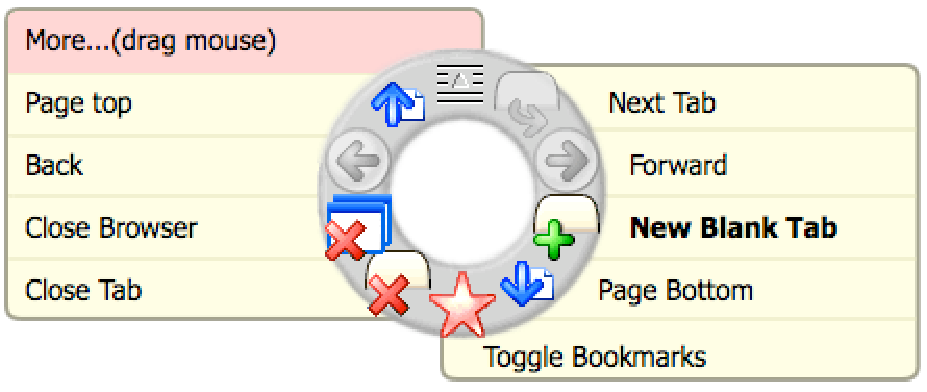
\includegraphics[angle=0, origin=c, width=2in]{img/pie-menu-browser.pdf}
    \label{fig:pie-menu-browser}
  }
  \subfigure[Autodesk Maya pie menu.] {
    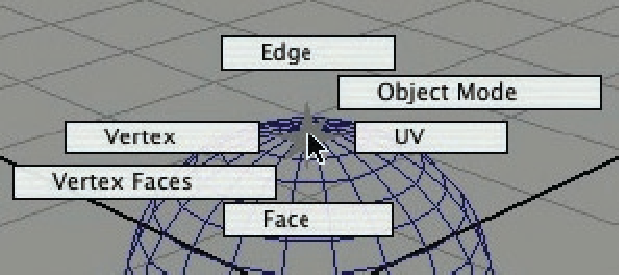
\includegraphics[angle=0, origin=c, width=2in]{img/pie-menu-maya.pdf}
    \label{fig:pie-menu-maya}
  }
  \caption{Pie menu implementations in two applications.}
  \label{fig:pie-menu}
\end{center}
\end{figure}

More natural interaction techniques must be developed in order to
reduce cognitive load. Several methods have been shown to work well
for pen applications. Marking menus are a good
example~\cite{kurtenbach-marking-menus}. Traditional menus provide a
list of options, growing downwards and to the right. For pen devices
with co-located input and output (such as a Tablet PC) the user's hand
may obscure the menu. Pie menus (a type of marking menu) appear
centered at the pointer location, with options distributed radially
(see Figure~\ref{fig:pie-menu}). The user's hand may still be
partially in the way, but at least part of the menu remains
visible. The benefit of the marking menu is that people can learn to
perform gestures without reading the option labels if the options
appear in consistent locations. The need for a visual menu eventually
disappears, leaving only the gesture. Pie menus are used in
applications such as Maya \cite{autodesk-web}, games such as the Sims
\cite{ea-sims}, and are available as add-ons to web browsers. This
approach works well, but has two drawbacks. First, it is not clear how
the menu should be invoked. Second, gestures must be discovered,
learned, and remembered.

Ramos \textit{et. al} further explored the use of pressure data for
pen based interaction~\cite{ramos-pressure-widgets}. In addition to
the stylus $(x,y)$ position, pressure serves as another dimension the
user can freely manipulate. For example, pressing lightly may produce
a menu with one set of options, while pressing hard offers a different
option set. Pressure could be effective as an input modality if used
appropriately, including haptic and visual feedback.

Traditional menus are typically invoked by clicking the mouse,
applying force orthogonal to the mouse's plane of operation, which
does not cause the mouse to move. Some computer styluses have barrel
buttons that allow users to ``right click'', but the force necessary
to depress the stylus button is liable to cause unintentional pen
movement, leading to mistakes~\cite{hinckley-input-technology}.

Hinckley \textit{et. al} suggest the use of delimiters to trigger
marking menus~\cite{hinckley-scriboli}. A delimiter is ``something
different'' in the pen input that the user is otherwise unlikely to
draw but is easy to remember. One example delimiter in their Scriboli
system is a pigtail mark, a loop made at the end of a selection
gesture. This fluid motion lets the user indicate target objects
followed by a command to apply to those objects.

Others have developed interface idioms for supporting pen and sketch
input. \textit{Gedrics} are gesture-driven icons for pen based
applications~\cite{geissler-gedrics}. Each Gedric is associated with a
class of tasks such as ``changing font properties'' in a text
editor. To invoke a command, the user draws a gesture on a Gedric. The
system recognizes the gesture, giving the icon meaning that can be
activated by tapping it. On the ``font'' Gedric, drawing a slanted
line might italicize selected text; drawing a vertical gesture from
the bottom to top increases text size. However, while Gedrics help
make some operations more convenient and reduce clutter on user
interfaces, they also require users to know how to turn their
intentions into a gesture. 

\begin{figure}
   \centering
   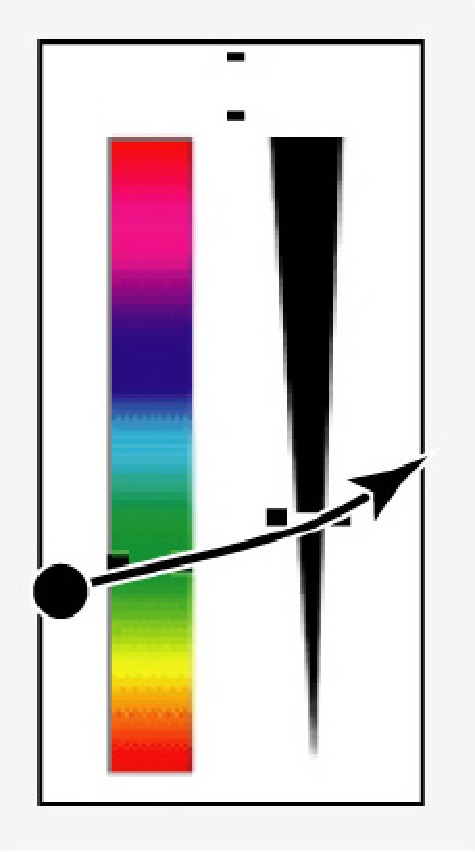
\includegraphics[width=1.2in]{img/crossy.pdf} 
   \caption{CrossY interface widgets let users change multiple
   parameters with a single stroke---pen color and thickness in
   this example.}
   \label{fig:crossy}
\end{figure}

While pointing and clicking is appropriate for tasks commonly
performed with mice, Accot and Zhai suggest ``crossing'' as an apt
technique for stylus interaction~\cite{accot-crossing}. The
experimental drawing program CrossY~\cite{apitz-crossy} demonstrates
interface widgets that support crossing. To activate a CrossY button,
the user draws a line from one side of the button to the
other. Crossing makes it easy to take multiple actions with a single
fluid motion, for example changing pen color and thickness by dragging
the pen across adjacent CrossY widgets (see Figure~\ref{fig:crossy}).

The inherent ambiguity of sketching is also present in pen based
interaction that is not intended to be sketchy, e.g. pressing a button
or choosing a menu item. When the user attempts to act on an object
the system may have to disambiguate the target. For example, when
pressing a button, the pen may accidentally slide off one into
another. This is called \textit{target
ambiguity}~\cite{mankoff-burlap,mankoff-oops}.

An alternative to mediating ambiguity is to preempt it. Pegasus and
Chateau~\cite{igarashi-pegasus,igarashi-suggestive} demonstrate a
\textit{suggestive interface} that predicts what the user will draw
and shows the outcomes of various possible actions. If a pick-list
mediator from BURLAP/OOPS is like asking you to clarify what you've
said, a suggestive interface is analogous to completing your sentence
before you finish. For example, Chateau's simplified domain of
architectural design~\cite{igarashi-suggestive} is constrained to
certain configurations of walls and beams known to produce good
results. This technique is appropriate when the domain has a highly
regular grammar or when structural properties such as symmetry may be
exploited. Tsang and colleagues use a suggestive interface for their
3D sketching system that can model shapes such as aircraft
hulls~\cite{tsang-3d-sketching}. The system provides an overlay that
guides users in providing additional sketch input. Users found this
conducive to providing precise input. The system uses the incomplete
sketch as a database query, finding similar drawings, and suggests
additional geometry that may be appropriate.

Bae's 3D curve modeling system demonstrates how several calligraphic
interaction techniques can be used together to provide a highly fluid
sketching environment~\cite{bae-ilovesketch}. The system, called
\nohyphens{ILoveSketch}, presents a physical sketchbook metaphor. Note
that like Sketchpad, input is provided using a stylus, optionally
modified by pressing physical buttons with the non-dominant hand
(Figure~\ref{fig:ilovesketch}). The interface lacks the familiar
on-screen buttons, scroll bars, and menus. Instead, users give
commands with gestures which are often context-sensitive. For example,
to browse earlier drawings the user ``peels'' back virtual pages by
dragging a corner; to erase an item the user draws a ``scratch-out''
gesture. Many techniques implemented in \nohyphens{ILoveSketch}
address challenges associated with sketching 3D objects. For example,
the system infers appropriate viewing angles by rotating or panning
based on the user's work.

\begin{figure}
   \centering
   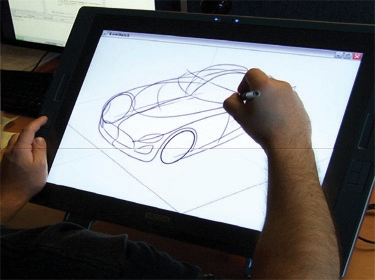
\includegraphics[width=2.5in]{img/ilovesketch.pdf} 
   \caption{ILoveSketch presents an ``as natural as possible''
     sketching system that brings together many calligraphic
     interaction techniques~\cite{bae-ilovesketch}.}
   \label{fig:ilovesketch}
\end{figure}

Alvarado provides a list of seven design guidelines for
developing \textit{Sketch Recognition User Interfaces}, or
SkRUIs~\cite{alvarado-skrui-guidelines}. These guidelines are:

\begin{small}
\begin{enumerate}
\item Display recognition results only when the user is done sketching.
\item Provide obvious indications to distinguish free sketching 
      from recognition.
\item Restrict recognition to a single domain until automatic domain 
      detection becomes feasible.
\item Incorporate pen based editing.
\item Sketching and editing should use distinct pen motions.
\item SkRUIs require large buttons.
\item The pen must always respond in real time.
\end{enumerate}
\end{small}

While WIMP interfaces have been widely used since the mid-1980s,
sketch-based interfaces remain to be adopted. To develop better
interaction guidelines, interface design patterns and toolkits, the
research community must continue to build and evaluate
sketching-centric applications.

\section{The ``mode problem''}
\label{sec:interaction-mode-problem}

User interfaces often interpret input differently depending on which
mode a program is in. For example, a structured graphics program may
have input modes such as \textit{select}, \textit{draw line},
or \textit{fill color}. Such a tool allows users to indicate
rectangular areas when the selection tool is active. The same program
also allows users to draw when the pencil tool is active. In both
cases the user presses a mouse button and drags the cursor. But the
program interprets user input in terms of the active tool. Sometimes
users are unaware of which mode the program is in, or are unsure how
to change to the desired mode. Managing modes often introduces
cognitive load by forcing users to think about the tool rather than
their work. This is called ``the mode
problem''~\cite{tesler-mode-problem}. It has been a challenge since
the beginning of interactive systems and is certainly not particular
to sketching software.

Sketchpad, arguably the first sketching system, addressed this by
letting the user control the mode with physical controls (buttons,
toggle switches, dials) with the left
hand~\cite{sutherland-sketchpad}. GRAIL users did not explicitly enter
modes to edit text and graphics. Instead, the meaning of user input
was inferred by analyzing ink and its
context~\cite{ellis-grail}. These two early systems represent opposite
extremes in ways to address the mode problem. Sketchpad's solution was
explicit mode changes using non-pen input; GRAIL's solution was
implicit mode changes done only with pen input.

There seems to be no clear ``right'' way to address the mode
problem. Implicit mode changes may seem more natural, but only if the
system correctly recognizes the user's intention. Recognition
techniques are error-prone. Many systems therefore provide a
combination of these two ways or impose drawing conventions.

Saund and Lank explored automatically recognizing mode based on the
user's input in context of what has already been
drawn~\cite{saund-inferred-mode}. Their \textit{inferred-mode
protocol} specifies an approach for analyzing the pen's trajectory and
determining if an action may be taken unambiguously. If the user's
intention is ambiguous, a mediator (such as those demonstrated by
BURLAP~\cite{mankoff-burlap}) provides the user with methods to
resolve ambiguity.

Li \textit{et. al} compared mode-switching techniques for pen based
user interfaces~\cite{li-mode-switching}. These techniques included
the pen's button, press and hold, using the non-dominant hand to press
a physical button, a novel pressure-based method, and using the eraser
end of the stylus. Interestingly, using the non-dominant hand to
switch modes was the fastest, the least error-prone, and best-liked
method. 

The ``press and hold'' approach is also used by
Schilit \textit{et. al}, who call this a ``dwell''
gesture~\cite{schilit-xlibris}.  Microsoft Windows for Tablet PCs uses
a dwell gesture for invoking right-click menus.

Scriboli's delimiters address the mode problem by allowing users to
seamlessly switch between which objects to operate on and which
commands to invoke~\cite{hinckley-scriboli}. For sketch-based systems
the mode problem arises partly because there are multiple types of pen
input. Some ink is intended to stay on the page and represents words,
pictures, or other model elements (\textit{model operations}). Other
pen input indicates selections or commands (\textit{environment
  operations}).

\begin{figure}
  \centering
  \subfigure[] {
    \label{fig:flowselection-1}
    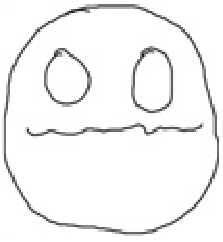
\includegraphics[origin=c,width=2.5cm]{img/flowselection-1.pdf} 
  }
  \subfigure[] {
    \label{fig:flowselection-2}
    
\includegraphics[width=2.5cm]{img/flowselection-2.pdf}
  }
  \subfigure[] {
    \label{fig:flowselection-3}
    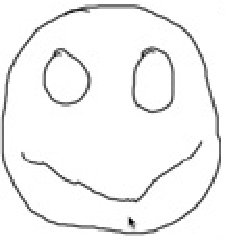
\includegraphics[origin=c,width=2.5cm]{img/flowselection-3.pdf} 
  }
  \subfigure[] { 
    \label{fig:flowselection-4}
    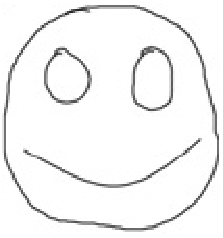
\includegraphics[origin=c,width=2.5cm]{img/flowselection-4.pdf} 
  }

  \caption{Flow selection's mode changes done by alternately holding
  and moving the stylus~\cite{johnson-flow-selection}. Here the user
  positions the stylus near the middle of the figure's mouth
  and \subref{fig:flowselection-2} moves it without lifting the
  pen \subref{fig:flowselection-3}. The user then holds the stylus
  still until the curve is smoothed \subref{fig:flowselection-4}
  before completing the process by lifting the
  pen.}  \label{fig:flow-selection}
\end{figure}


Flow selection~\cite{johnson-flow-selection} allows users to
seamlessly change modes from drawing to selecting with a dwell
gesture. Subsequent operations (such as moving part of a line) are
performed by moving the stylus without lifting up. In the example in
Figure~\ref{fig:flow-selection}, the selection strength depends on
distance to the place the user is pressing and how long the stylus has
been held down. Selection strength is then used by subsequent
operations such as moving or smoothing.

\section{Application areas of sketching}
\label{sec:interaction-application-areas}

\subsection{Problem solving}

Sketching supports everyday problem solving. A homeowner may estimate
financial figures on the back of an envelope when managing household
funds. A college student may draw a dorm room floor plan with
furniture in various configurations to determine what is possible and
desirable. Pencil and paper support these quick calculations very
well.

One problem solving domain addressed by sketching systems is
mathematics. MathPad$^{2}$~\cite{laviola-mathpad} and
MathBrush~\cite{labahn-mathbrush} let students draw pictures of
natural phenomena and relate them to equations. For example, a
physical system involving a mass on a spring can be represented with a
drawing as well as with an equation as in
Figure~\ref{fig:mathpad2}. The drawing directly communicates
qualitative aspects about the system such as location and size of
elements, while the equation governs the quantitative properties such
as the weight's mass~$m$, the spring constant~$k$ and the time
parameter's range~$t$.

\begin{figure}[h]
   \centering 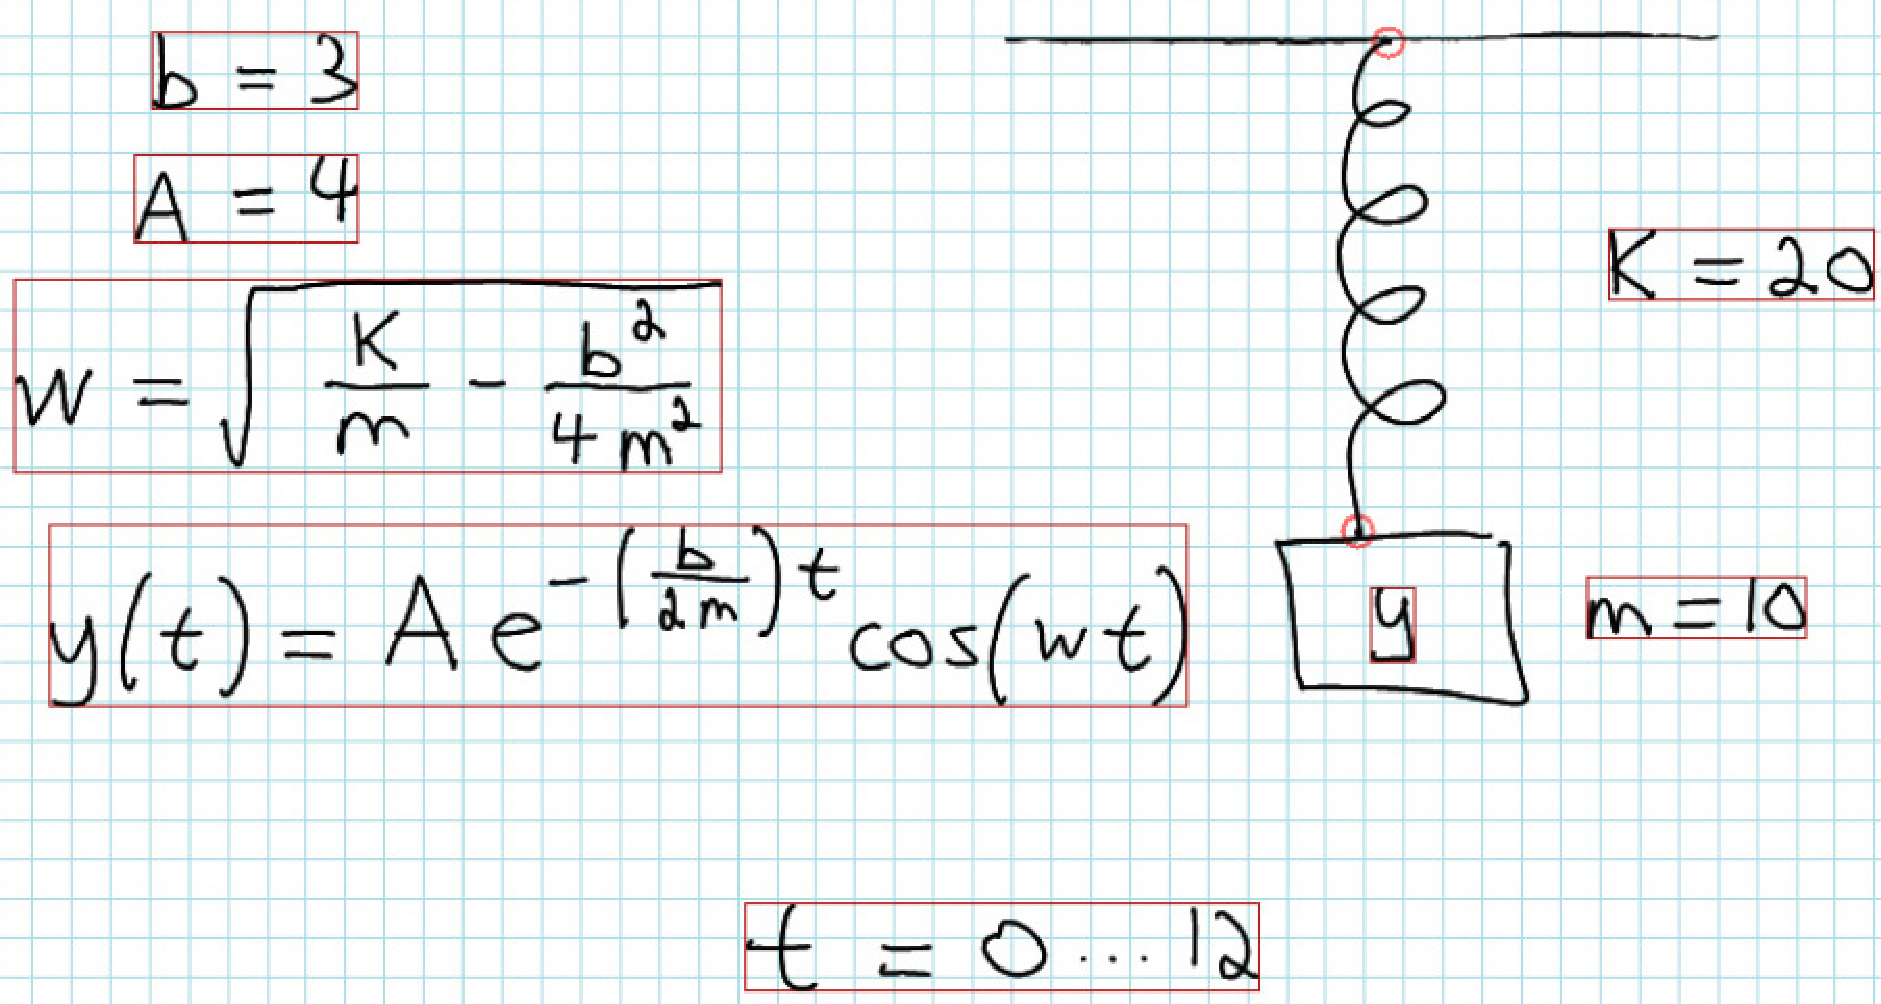
\includegraphics[width=3in]{img/mathpad2.pdf} 

   \caption{A MathPad$^{2}$ sketch showing hand-written equations
   corresponding to the drawing of the mass-and-spring system at
   right, which the system can animate.}

   \label{fig:mathpad2}
\end{figure}

Many sketching systems allow users to simulate models. The
MathPad$^{2}$ sketch in Figure~\ref{fig:mathpad2} can be set into
motion using the drawing as the initial condition, and the values $m,
k,$ and $t$ to control the animation.

Another example of problem solving addressed by sketching is editing
and annotating written documents using ink based writing or
gestures. XLibris is an electronic book that supports users in reading
documents and keeping notes on the pages, which the system
automatically organizes~\cite{schilit-xlibris}. XLibris also
recognizes certain ink commands as search requests. For example, say
an XLibris user reading this paragraph circled, underlined, or
highlighted the phrase ``electronic book''. This action silently
triggers a database query. If a strong match is found, a link appears
in the margin along with the word's definition.

\subsection{Sketch-based prototyping}
\label{sec:interaction-prototype-computer}

Sketching itself can be a form of prototyping. For example, user
interface designers often build low-fidelity paper prototypes to use
for cognitive walkthroughs or usabilty studies. The `sketchy'
appearance may facilitate brainstorming or encourage people to make
multiple interpretations of what the sketch
means~\cite{do-design-sketches-tools}. Alternately, designers may draw
to unambiguously communicate specific
designs~\cite{newman-web-designers}.

Designers draw diagrams of how components fit together in order to
better understand how to make things. At some point designers can move
past sketching and build something---a user interface, a physical
mechanism, a computer program. Before the final product is built,
several prototypes are made to help clarify the problem domain,
manufacturing constraints, usability issues, and so on. Designers
often ``go back to the drawing board'', iteratively sketching and
building prototypes.

Low-fidelity renderings of interfaces encourage discussion on the
high-level functions the UI is intended to support. Conversely,
high-fidelity prototypes encourage discussion of details that are not
important during brainstorming or early
prototyping~\cite{wong-rr-prototypes,black-fidelity}.

SILK (Sketching Interfaces Like Krazy) allows designers to draw user
interfaces and storyboards and then interact with
them~\cite{landay-silk}. SILK recognizes sketches of a limited set of
common user interface elements such as buttons, scroll bars, and text
areas. It then transforms the sketch into a high-fidelity version of
their drawn UI in the look-and-feel of their choice. The user may
elect to retain the sketchy look and still interact with the
recognized drawing. The sketch-to-prototype process is fast: users
created an interface with SILK in one fifth of the time they needed to
make the same interface with a structured interface builder.

DENIM is a system for prototyping web sites and individual page
layouts~\cite{lin-denim}. DENIM allows designers to informally and
incrementally create structures, first starting at one level of
granularity, then moving up or down as appropriate. The ability to
`zoom' from level to level is conducive to iterative web site design.

Other sketch-based systems have been developed for prototyping
computer-based models including animations with K-Sketch, multimedia
authoring with DEMAIS, and software development with
MaramaSketch~\cite{davis-k-sketch,bailey-demais,grundy-maramasketch}. These
tools allow designers to build prototypes or storyboards of dynamic
systems by creating sketches according to conventional visual
languages.

One important property of physical sketches is their ability to record
how a particular design evolved. Designers often keep journals of
drawings and refer to them for reflection. Electronic sketching
systems like SILK, ART019~\cite{yamamoto-art019}, and
NetDraw~\cite{qian-netdraw} support capturing and retrieving design
histories of drawn objects.

\subsection{Sketching 3D artifacts}
\label{sec:interaction-prototype-fab}

SILK, DENIM, and similar systems explored prototyping designs for
electronic media. Another class of sketching systems supports rapid
development of physical artifacts. Because physical objects are three
dimensional, sketching systems targeting such output frequently
involve 3D modeling.

SKETCH~\cite{zeleznik-sketch} is a 3D modeling system that
accepts gestural input to perform modeling operations, rather than a
traditional menu-based approach. The implementation described assumes
a 3-button mouse as input, but the authors suggest that pen input
would be better. The multiple buttons are used to address the mode
problem, with shape operations performed with the left mouse button
and camera operations with the right mouse button. SKETCH-N-MAKE, an
``art to part'' CAD system, added the ability to produce physical
output~\cite{bloomenthal-sketch-n-make}.

SKETCH (and SKETCH-N-MAKE) define the characteristics of the model via
a sequence of operations (extruding, cutting, etc.) on an existing
model. This approach contrasts with a freeform drawing approach
whereby designers draw shapes in 2D and the CAD system derives a three
dimensional model. The freeform approach feels more ``natural'',
approximating and augmenting pencil and paper.

Recently there has been progress in developing prototypes that
construct 3D models based on freehand 2D
sketches~\cite{lipson-correlation,masry-3d-sketch}. These systems
allow designers to directly specify shapes as they are conventionally
drawn, rather than relying on mapping gestures to modeling commands.

Rapid prototyping machinery has become affordable. This gives people
additional tools for making things. The \textit{Furniture Factory}
and \textit{Designosaur}~\cite{oh-fab} projects are ``sketch-to-fab''
systems that enable people, even children, to design simple artifacts
such as doll house furniture or dinosaur skeleton models. The
Furniture Factory recognizes the 2D sketch as adjacent orthogonal
planes, and selects appropriate jointing, leading to a CAD model
suitable for manufacture on a laser cutter. Designosaur users sketch
shapes of wooden `bones' and indicate locations for the bones to notch
together.

\section{Sketching in playful applications}

Most of the systems described above have concerned the production of
functional artifacts such as web sites, mechanisms or math
equations. We can learn a lot (even about ``serious'' interactive
systems) by building and evaluating systems that are playful.

ART019~\cite{yamamoto-art019} explores a novel sketch-based form of
interaction for artists. It provides the ability to visualize drawings
over time and easily combine model states from different moments in
the drawing's creation history. For example, an artist may select a
portion of a sketch by \textit{when} strokes were applied, rather
than \textit{where} they were applied. DiFiore and Van
Reeth~\cite{difiore-sketching-artistic} describe an interface for
artistic sketch input for an animation tool that is as fluid as
pencil-and-paper while giving animators the added ability to freely
deform and edit drawings in an artful manner.

\begin{figure}
  \centering
  \subfigure[Crayon Physics Deluxe] { 
    \label{fig:fun-crayon} 
    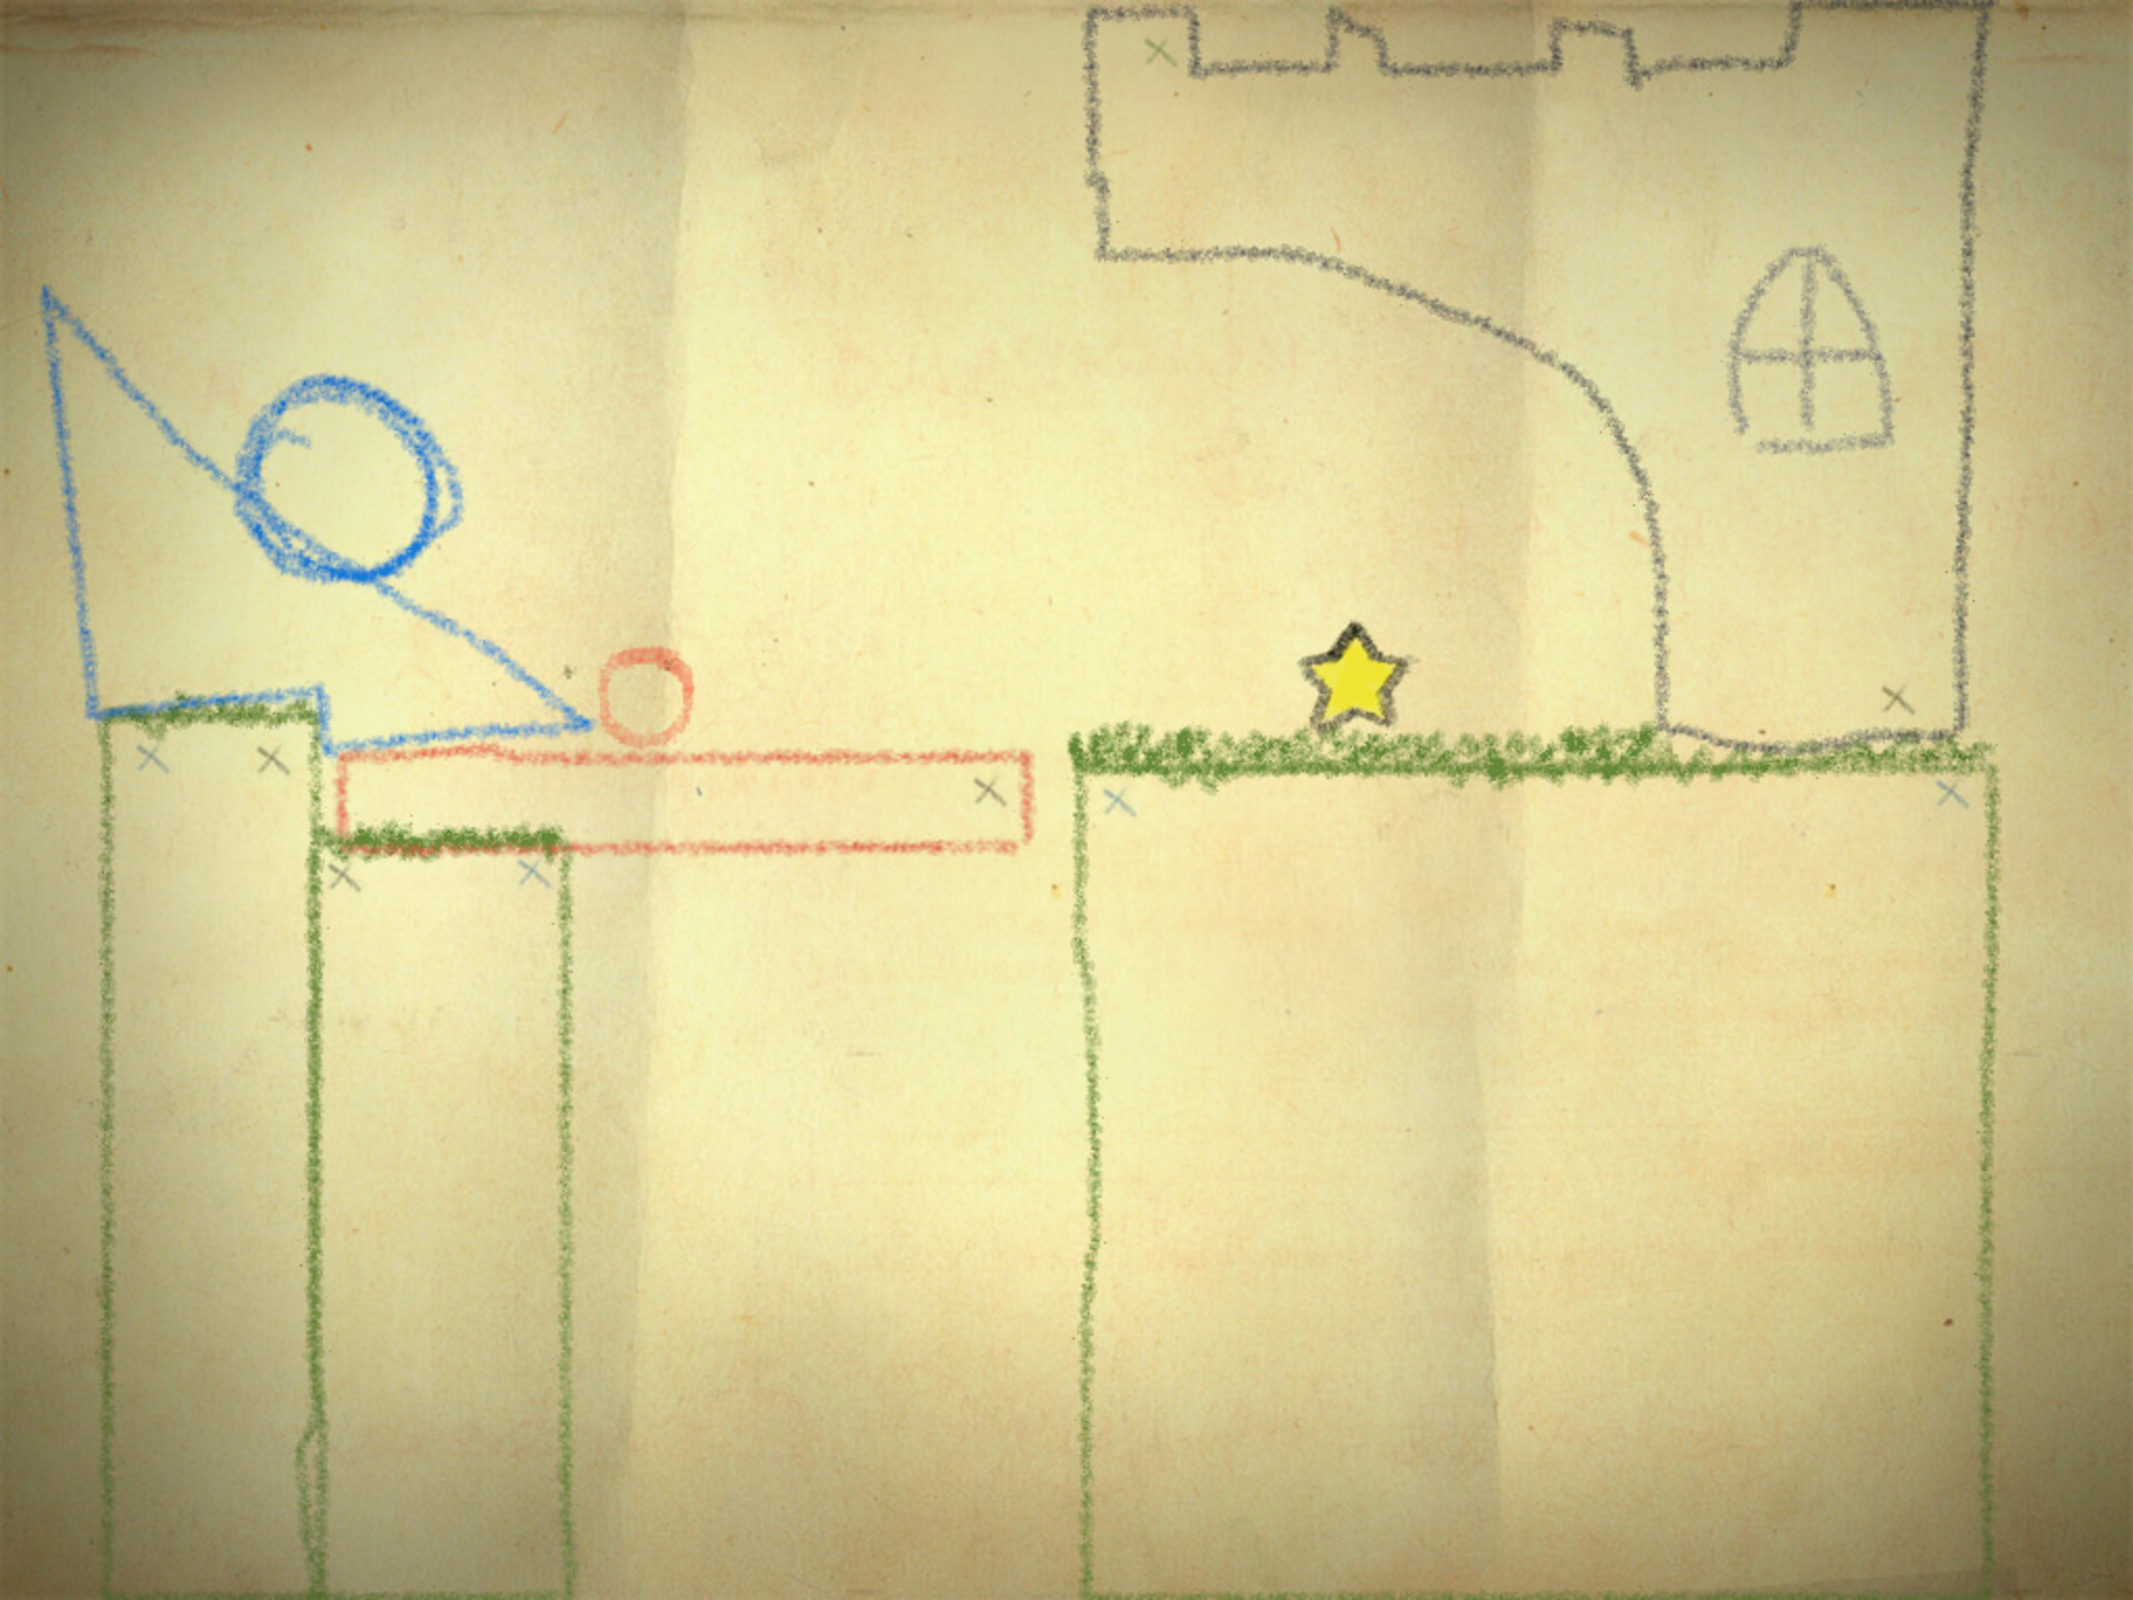
\includegraphics[width=4.5cm]{img/crayon_deluxe.pdf} 
  }
  \subfigure[Phun] {
    \label{fig:fun-phun} 
    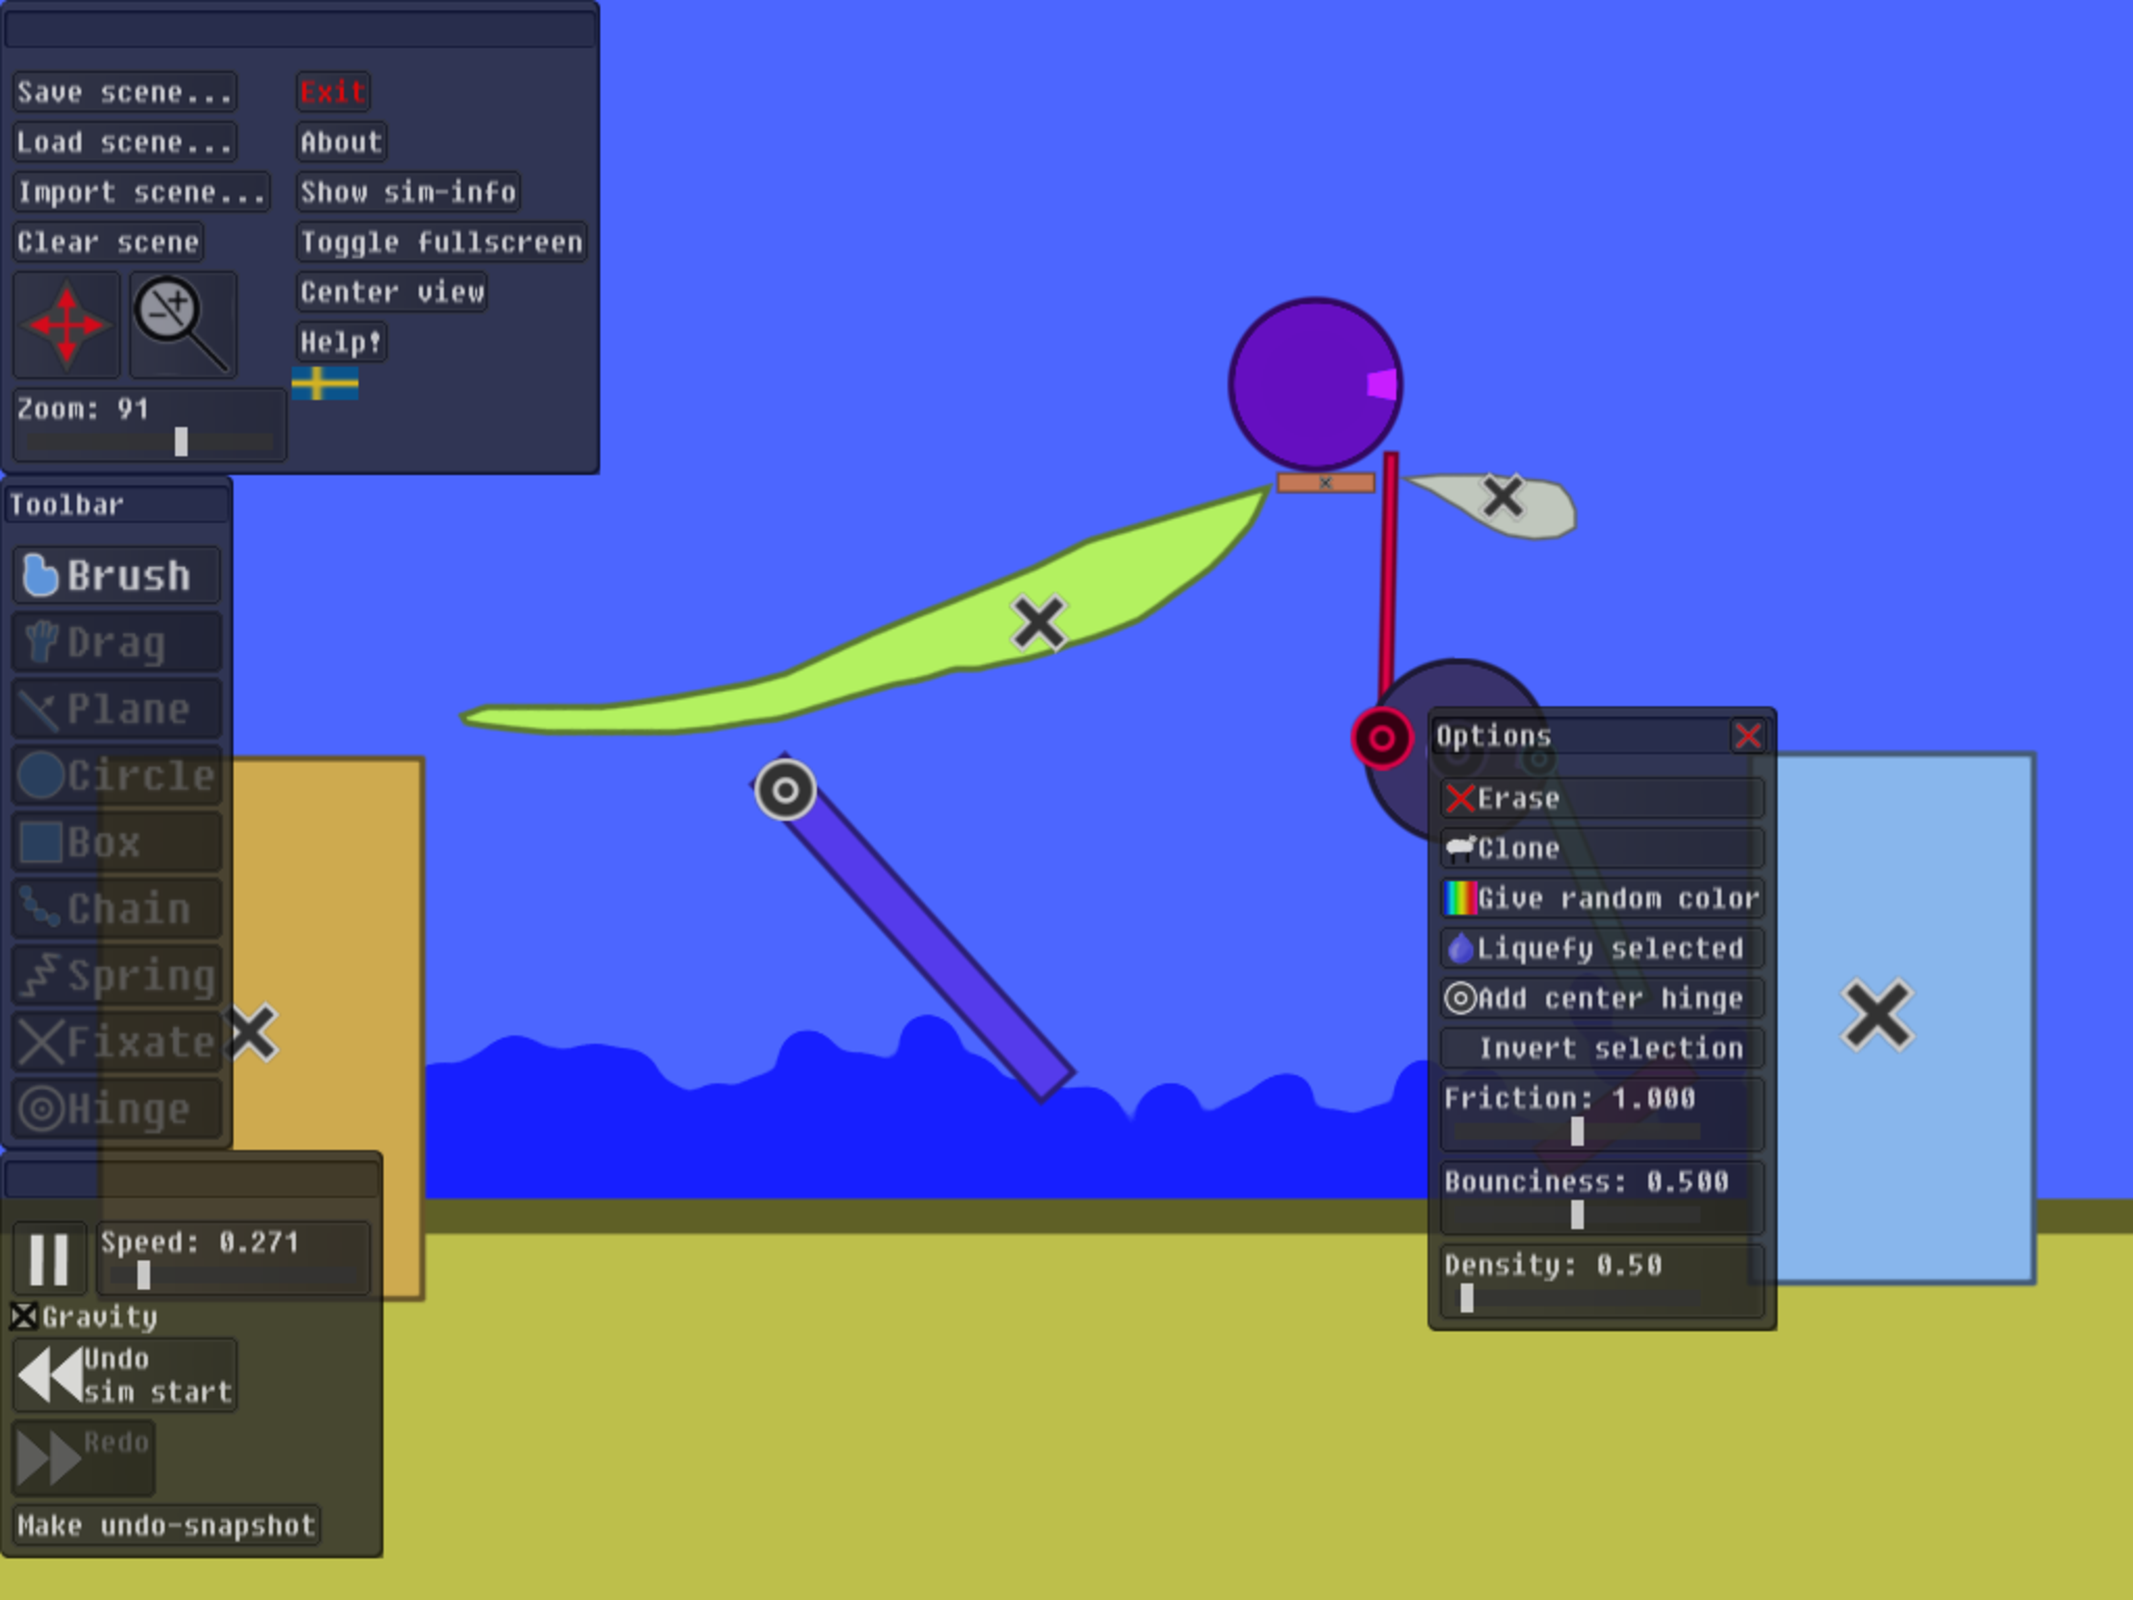
\includegraphics[width=4.5cm]{img/phun.pdf}
  }
  \caption{Two entertaining sketch-based physics simulation programs. Note the difference in how the programs render objects.}
  \label{fig:fun}
\end{figure}


Crayon Physics Deluxe and Phun are aptly-named sketching programs
wherein users draw shapes that are recognized as rigid bodies in a
physical simulation~\cite{crayon-physics-deluxe,ernerfeldt-phun}. The
user controls game play by drawing shapes that interact with one
another, subject to physical constraints such as gravity and rigid
collisions (see Figure~\ref{fig:fun}).

Paulson \textit{et. al} present a series of entertaining, educational
sketch-based systems for children to learn by
drawing~\cite{paulson-edu-sketch-games}. Their APPLES system lets
users draw elements such as planets, black holes, and arrows
representing initial velocity vectors. The recognized drawing then
becomes alive, simulating gravitational pull and elastic collisions.

Another playful calligraphic application is Plushie, a system for
designing stuffed toys~\cite{mori-plushie}. Plushie users draw shapes
that automatically turn into blobby, 3D objects rendered with
cartoon-like, non-photorealistic rendering. The system provides an
intuitive drawing environment where people can make engaging, complex
3D models.

Like Plushie, FiberMesh builds on prior work by Igarashi and
colleagues~\cite{nealen-fibermesh,igarashi-smooth}. FiberMesh enables
users to edit 3D free-form models. Users enter one of several modes
including deforming, rubbing, erasing, and type change. All strokes
remain on the model, giving the user controls for later manipulation.

The ``fun'' applications presented here provide the basis for serious
research. The act of drawing---even if it is a simple doodle---may
help to clarify the designer's
thoughts~\cite{cross-natural-intelligence}.  One participant in
Nealen's informal user study said, ``One great thing about this system is
that one can start doodling without having a specific goal in mind, as
if doodling on paper. One can just create something by drawing a
stroke, and then gradually deform it guided by serendipity, which is
very important for creative work~\cite{nealen-fibermesh}.'' 

\vspace{12pt}

This section has discussed interaction topics of computational support
for sketching. We began by presenting interaction concerning
recognition. This includes ways for handling recognition errors, and
how the system can react to sketch input and present interpretation
results to the user. Several toolkits for developing sketch based
software were presented. Application areas for supporting human
communication and design were described, with focus on areas where
sketching is particularly useful. We discussed low-level interaction
methods such as how users may select and act on objects, or how they
may explicitly or implicitly enter modes.


\newpage
\chapter{Challenges and Opportunities}
\label{sec:summary}

In the preceding five sections we have reviewed work on computational
support for sketching in design, beginning with GRAIL and Sketchpad in
the 1960s through work that is going on today. We have viewed the
field from various aspects: studies of ``traditional'' design
sketching done on paper without benefit of computation; hardware that
has been employed for computer supported sketching, techniques for,
and management of sketch recognition; and interaction in sketch based
design software. Although we attempt in this review to cover the main
themes in computer supported sketching for design, the field has grown
large and diverse. We cannot hope to have captured all worthy and
relevant work.

Our efforts in assembling this review began with a question: After
forty years of research on computational support for sketching, why
are there so few real world applications of this technology? Although
the mouse has dominated computer interfaces since 1980, we see no sign
that in daily life people are ceasing to draw with pencil and marker,
on paper, and on whiteboards. Indeed, people draw on every available
surface. We posit that if computational support for sketching really
worked, it would be more widely adopted in a variety of applications
and domains. As this has not yet happened, we asked ourselves: What is
the state of the art today, and what obstacles must be overcome before
freehand sketching interaction will make its way from the research
laboratory into the world of everyday use?

We found no simple single answer. However, our review of the
literature in this field reveals research directions---and in some
cases, challenges---in several areas that if resolved provides
opportunities to develop successful real world applications. We
summarize these below. Overall we maintain the optimistic outlook that
the day of real-world sketching interfaces is still to come---whether
just around the corner or a decade or more away. Each year we see a
growing number of published papers and research projects. Hardware
continues to advance, albeit somewhat more slowly. Further, the
research community working on sketch based interaction is growing both
in size and in diversity of backgrounds.

\section{Future work in understanding traditional sketching}
\label{sec:summary-three-areas}

Sketch based software for design depends on research in two main
areas. The first area is an understanding of the roles and uses of
sketching in design: why, when, and how designers make quick drawings,
and the role they play in the enterprise of designing. The second area
is an understanding of the mechanics of sketching---how people make
meaningful marks with a stylus. Research in these closely related
topics can foster a better understanding of the computational
mechanisms that can be brought to bear to support, in various ways,
the processes of sketching for design.

\subsection{Sketching in design}
The importance of sketching in design is asserted frequently in the
literature, though few studies (including our own) go further than
observing, as an argument for the authors' pen based software project,
that designers sketch. Yet if we are to build sketching software that
is truly useful for designers, we must gain a more systematic
understanding of the ways that designers make diagrams, drawings, and
sketches, how these representations serve design reasoning, how and
what they communicate, and how they can be integrated with other
knowledge and expertise. We cannot entirely separate the study of
sketching---as medium---from the study of design processes. Thus
research in computer support for sketching can benefit by engaging
designers and design researchers. Empirical studies of designers
sketching, ethnographies, and analyses of user needs have already
added to our knowledge. Nevertheless a thorough understanding of the
functions of sketching in design will come only when we also engage
designers in our quest.

\subsection{Mechanics of sketching}
The mechanics of drawing and sketching is the second area where
advances in research will lead to real world applications. There is a
small but fascinating body of literature on how people draw things: we
mentioned van Sommers' studies and there are others. Previously, film
and video has been used to look closely at drawing mechanics. Now, pen
technologies can fuel empirical studies on drawing ergonomics using
Anoto, Wacom, or similar capture devices. These technologies can
record drawing behavior that may be analyzed to better understand
patterns and preferences for certain kinds of drawing tasks. What
sequence do people choose in making a drawing, and what governs this
choice? What, if any, is the relationship between pen speed, pressure,
and the designer's level of confidence or certainty in the drawing?
Answering these and other questions about drawing mechanics can lead,
among other things, to software that can more effectively use these
input data in building a more accurate model of the designer's
actions.

Better knowledge about drawing mechanics can also inform the
development of input and output hardware for sketching in design. We
have seen hardware platforms move from light pens and CRTs, to
expensive tethered digitizing surfaces, to low-cost tablets integrated
with displays, digitizing whiteboards, and most recently e-ink and
electronic paper. For input technologies, costs drop as resolution,
reliability, and portability improve. Output technologies also improve
in resolution, color capability, power consumption, and readability
under diverse lighting conditions. The relatively recent introduction
of Anoto's technology, introduced in 1998, reminds us that radically
different approaches in hardware are possible and can lead to quite
different applications. Two-handed interaction~\cite{kurtenbach-t3} is
valuable in certain tasks, as is the ability to draw on arbitrary
surfaces or in space~\cite{schkolne-shape-sculpt}. It is easy to
underestimate the effects of hardware on the performance of sketching
systems: subtle ergonomic factors such as display screen parallax or
the pen's feel on the drawing surface contribute to user
satisfaction. Designers want to be comfortable drawing for extended
periods of time, and even casual users are surprisingly sensitive to
pen and surface ergonomics.

Under the broad rubric of computational mechanisms to support
sketching in design, we have looked at (in
Section~\ref{sec:recognition}) managing and integrating recognition
into sketch based interfaces, and (in Section~\ref{sec:interaction})
interaction techniques specific to sketching.

\section{Future work in computational support for sketching}

\subsection{Recognition}

Sketch recognition is a cousin to speech and gesture recognition, and
there are issues common to all recognition based interaction, for
example segmentation, grouping, and managing conflicts, correction,
context, and n-best lists. Generally, the sketch recognition community
could benefit from a close comparative study of research on
recognition in these other modalities. We found no empirical data on
what accuracy rate is acceptable in sketch recognition: How good must
a recognizer be? Although this is likely to vary according to user and
circumstance, the field would benefit by having benchmark data on
acceptable accuracy in sketch recognition, similar to studies of
acceptance of handwriting recognition accuracy.

Recognizer training is another area where research could advance
support for sketching. Users are reluctant to devote time to training
a recognizer, and so methods for incorporating training into ordinary
use scenarios would be advantageous. Machine learning techniques might
be applied to extract patterns from sketch data obtained from large
numbers of users. When is it necessary to train a recognizer for
individual users; when can a standard scheme serve all users? And when
training is necessary, what interfaces are users most willing to
tolerate? How can the number of needed training samples be minimized?
Comparative usability and performance evaluations of training methods
could be helpful.

Also related to recognition, when and under what circumstances should
an application attempt recognition? Just how eager or lazy should a
recognition engine be? When to be eager; when to be lazy? What
heuristics can an application use to determine its recognition
strategies? To what extent, and using what methods, can a system's
knowledge of context support recognition? And finally, although many
different approaches to recognition have been pursued, the challenge
of recognizing sketches, whether domain-centric or domain-independent,
remains an open problem. 

A special (but important) case of sketch recognition is the problem of
generating three-dimensional models from two-dimensional
sketches. Again, many efforts have tackled particular kinds of
2D-to-3D sketch recognition. Yet specific constraints bound the
capabilities of each of these projects: some systems make assumptions
of orthonormal geometry; others handle curved surfaces. We are still
far from a general purpose system for generating three dimensional
models from sketches. The challenges here include dealing with
incomplete drawings (e.g., lines truncated by the edge of the sketch);
incorrect drawings (not made to correct isometry or perspective); the
use of shading, hatching, and line weight to inform
model-construction. Here we also distinguish between projects that aim
to recognize and parse projection drawings made according to the
traditional conventions, and those (like SKETCH~\cite{zeleznik-sketch}
and SketchUp~\cite{google-sketchup}) that use an artificial language
of gestural commands to construct models.

\subsection{Interaction techniques}

Another broad area where research can advance software support for
sketching in design is interaction techniques specifically tuned for
the pen. The early work at PARC that produced the WIMP interface led
to widely adopted conventions for using the mouse to interact with
applications. We have yet to see a similar set of conventions emerge
for using the pen to interact with applications, though as we saw in
Section \ref{sec:interaction}, some work has been done along these
lines. Pen interaction techniques might leverage input data such as
pressure~\cite{ramos-pressure-widgets} and pen angle, in addition to
the customary position, timing, and pen-up, pen-down events. It may be
fruitful also to look at the design of screen widgets specifically for
use with the pen, rather than assuming that the widgets that work for
the mouse are equally suited for pen based interaction. And work with
gestures such as the ``pigtail'' or the technique of ``crossing''
screen items suggests that developing and adopting a conventional
language of pen gestures may be
helpful~\cite{hinckley-scriboli,apitz-crossy}.

Stepping up a level from the pen and screen, support for sketching
will require other interaction techniques. For example, managing
recognition errors and ambiguities in a sketching program without
unduly distracting the designer remains a challenge. Research on
interruption management may be useful: the system could assess the
user's state and decide when is an appropriate time to query for
resolving an error, conflict, or ambiguity.

\subsection{Application architectures}

Perhaps one of the greatest obstacles to widespread adoption of
sketching interaction is the underlying architecture of application
software and the software engineering assumptions that this entails. A
strength of sketching is that it can convey decisions on a spectrum
from ambiguity and vagueness to precision and certainty. However, as
long as the underlying software does not support such a spectrum, it
will be difficult to take advantage of this feature. That is, whatever
degree of ambiguity or precision the user may wish to convey through
the sketch will be resolved before the application gets hold of it. In
this review we have touched many times on the idea that sketches can
capture the user's level of commitment and precision, but until
application software can use this information, the system's capacity
to capture and convey it is wasted. Here we contrast speech and sketch
recognition: It is a fair assumption that a speaker has intended to
make a specific and precise utterance, and it is the job of the
listener to recognize what that was. As we've pointed out, in design
this is not always the case.

Sketching, however, does not only happen at the early stages of
designing. Designers sketch throughout the process, and so software
must also be able to capture and use sketch input even during later
stage design. The earliest, exploratory sketches may convey a wide
range of alternatives quickly. Drawings made in concluding phases
resolve detail and entail highly precise decision making.  Effective
sketch based applications must be able to support designers throughout
this process. 

In the vein of innovative application architectures that take
advantage of sketching input, it is worth remarking that many of the
innovations in Sketchpad were programming language ideas, not what we
would now see as HCI ideas. The software architecture of Sketchpad---a
constraint solver at its core, an object-like representation of
prototypes and instances---these were deeply integrated into the
design of the program. It may take more than wrapping existing
applications with a ``sketching interface'' in order to reap the
advantages of pen based interaction.

\subsection{Toolkits}

Most of the systems we reviewed here were built from scratch, using
only the most basic device and graphics libraries. Building from the
ground up can allow more divergent and potentially innovative
work. However, this comes at a heavy cost: a great deal of redundant
effort is spent by the sketching research community building similar
low-level functionality. In order to advance the field and build more
robust and sharable sketching applications, programmers can rely on
toolkits and libraries to perform many of the mundane and common
tasks. Several toolkits have been proposed and developed (e.g. SATIN
and InkKit~\cite{hong-satin,plimmer-inkkit}) but these have not gained
widespread acceptance.  It would be worth looking into why more
researchers and developers have not adopted these toolkits. What would
be the required characteristics of a successful toolkit for
sketching---both research prototypes and full-fledged
applications---remains an open question.

\section{Conclusion: in support of visual thinking}

Computational support for sketching has a long and interesting history
dating back to the early days of computing. Some of the first
graphical interfaces in the 1960s demonstrated compelling features
that even today are not wholly integrated into pen computing. Despite
advances in hardware (digitizing whiteboards, the
Wacom\texttrademark\ ~\cite{wacom} and Anoto pen technologies, the
Tablet PC) sketching remains a niche area. Perhaps it always will. On
the other hand, it may be that overcoming a number of obstacles would
make pen based sketch interaction far more attractive in a range of
application areas. People, after all, still draw.

Certainly for designers---and by this we mean not only those in the
``artistic'' or ``creative'' professions but also chemical,
electrical, mechanical engineers, economists, anyone who uses
graphical representations in their work---better computer support for
sketching would be a boon. Arguably, sketching and diagramming is not
just a matter of recording geometry of ideas that have been worked out
in the head. Rather, as Arnheim put it, drawing is a medium for visual
thinking~\cite{arnheim-visthink}. Seen in this way, supporting
sketching for design goes beyond strategies for more accurately
capturing pen strokes or ink, or tuning recognition. Truly inspired
work on computational support for sketching will see its task as
supporting designers---and all users---in thinking visually.





\newpage
\bibliographystyle{nowsort}
\bibliography{sketch-bibliography}

\end{document}
